\batchmode
\makeatletter
\def\input@path{{/dump/writingswork/draftthesis//}}
\makeatother
\documentclass[12pt,english]{report}\usepackage[]{graphicx}\usepackage[]{color}
%% maxwidth is the original width if it is less than linewidth
%% otherwise use linewidth (to make sure the graphics do not exceed the margin)
\makeatletter
\def\maxwidth{ %
  \ifdim\Gin@nat@width>\linewidth
    \linewidth
  \else
    \Gin@nat@width
  \fi
}
\makeatother

\definecolor{fgcolor}{rgb}{0.345, 0.345, 0.345}
\newcommand{\hlnum}[1]{\textcolor[rgb]{0.686,0.059,0.569}{#1}}%
\newcommand{\hlstr}[1]{\textcolor[rgb]{0.192,0.494,0.8}{#1}}%
\newcommand{\hlcom}[1]{\textcolor[rgb]{0.678,0.584,0.686}{\textit{#1}}}%
\newcommand{\hlopt}[1]{\textcolor[rgb]{0,0,0}{#1}}%
\newcommand{\hlstd}[1]{\textcolor[rgb]{0.345,0.345,0.345}{#1}}%
\newcommand{\hlkwa}[1]{\textcolor[rgb]{0.161,0.373,0.58}{\textbf{#1}}}%
\newcommand{\hlkwb}[1]{\textcolor[rgb]{0.69,0.353,0.396}{#1}}%
\newcommand{\hlkwc}[1]{\textcolor[rgb]{0.333,0.667,0.333}{#1}}%
\newcommand{\hlkwd}[1]{\textcolor[rgb]{0.737,0.353,0.396}{\textbf{#1}}}%

\usepackage{framed}
\makeatletter
\newenvironment{kframe}{%
 \def\at@end@of@kframe{}%
 \ifinner\ifhmode%
  \def\at@end@of@kframe{\end{minipage}}%
  \begin{minipage}{\columnwidth}%
 \fi\fi%
 \def\FrameCommand##1{\hskip\@totalleftmargin \hskip-\fboxsep
 \colorbox{shadecolor}{##1}\hskip-\fboxsep
     % There is no \\@totalrightmargin, so:
     \hskip-\linewidth \hskip-\@totalleftmargin \hskip\columnwidth}%
 \MakeFramed {\advance\hsize-\width
   \@totalleftmargin\z@ \linewidth\hsize
   \@setminipage}}%
 {\par\unskip\endMakeFramed%
 \at@end@of@kframe}
\makeatother

\definecolor{shadecolor}{rgb}{.97, .97, .97}
\definecolor{messagecolor}{rgb}{0, 0, 0}
\definecolor{warningcolor}{rgb}{1, 0, 1}
\definecolor{errorcolor}{rgb}{1, 0, 0}
\newenvironment{knitrout}{}{} % an empty environment to be redefined in TeX

\usepackage{alltt}
\usepackage{fontspec}
\setmainfont[Ligatures=TeX]{Georgia}
\setsansfont[Ligatures=TeX]{Arial}
\setmonofont{Liberation Mono}
\usepackage[letterpaper]{geometry}
\geometry{verbose,tmargin=1in,bmargin=0.75in,lmargin=1.5in,rmargin=1in}
\setcounter{secnumdepth}{0}
\usepackage{color}
\definecolor{note_fontcolor}{rgb}{0.800781, 0.800781, 0.800781}
\usepackage{babel}
\usepackage{array}
\usepackage{graphicx}
\usepackage{setspace}
\usepackage[numbers]{natbib}
\usepackage{nomencl}
% the following is useful when we have the old nomencl.sty package
\providecommand{\printnomenclature}{\printglossary}
\providecommand{\makenomenclature}{\makeglossary}
\makenomenclature
\doublespacing
\usepackage[unicode=true,pdfusetitle,
 bookmarks=true,bookmarksnumbered=false,bookmarksopen=false,
 breaklinks=false,pdfborder={0 0 0},backref=false,colorlinks=false]
 {hyperref}

\makeatletter

%%%%%%%%%%%%%%%%%%%%%%%%%%%%%% LyX specific LaTeX commands.
%% Because html converters don't know tabularnewline
\providecommand{\tabularnewline}{\\}
%% The greyedout annotation environment
\newenvironment{lyxgreyedout}
  {\textcolor{note_fontcolor}\bgroup\ignorespaces}
  {\ignorespacesafterend\egroup}

%%%%%%%%%%%%%%%%%%%%%%%%%%%%%% User specified LaTeX commands.
\usepackage{ifxetex,ifluatex}
\newif\ifxetexorluatex
\ifxetex
  \xetexorluatextrue
\else
  \ifluatex
    \xetexorluatextrue
  \else
    \xetexorluatexfalse
  \fi
\fi
\ifxetexorluatex
  \usepackage{fontspec}
\else
   \usepackage[T1]{fontenc}
\fi
\usepackage[normalem]{ulem}
\usepackage[utf8]{inputenc}
\usepackage{textcomp,lipsum,comment,tabularx,array,indentfirst}
\usepackage{caption,setspace}
\captionsetup{font={stretch=1.3}}
\usepackage[section]{tocbibind}
\usepackage[version=3]{mhchem}
\includecomment{comment}
\usepackage[per-mode = symbol]{siunitx}
\DeclareSIUnit\curie{Ci}
\DeclareSIUnit\molar{M}
\setlength{\bibsep}{2pt}
\raggedright
\raggedbottom
\setlength{\parindent}{.3in}
\usepackage{chngcntr}
\counterwithout{figure}{chapter}
\counterwithout{table}{chapter}
\renewcommand{\nomname}{Abbreviations}
\def\nompreamble{\addcontentsline{toc}{section}{\nomname}\markboth{\nomname}{\nomname}}
\let\nomenclOrig\nomenclature
\renewcommand*{\nomenclature}[3][]{#2\nomenclOrig[#1]{#2}{#3}}
\renewcommand{\@makechapterhead}[1]{
 {\parindent \z@ \centering \normalfont
  \ifnum 
     \c@secnumdepth >\m@ne \bfseries \thechapter .
  \fi
  \bfseries \MakeUppercase{ #1 }\par
  \nobreak
  \vskip 20\p@
 }
}
\renewcommand\section{\@startsection {section}{1}{\z@}
  {-3.5ex \@plus -1ex \@minus -.2ex}
  {2.3ex \@plus.2ex}
  {\centering \normalfont \bfseries}}
\usepackage{fancyhdr}
\fancypagestyle{preamblepages}
{
  \fancyhf{}
  \renewcommand{\headrulewidth}{0pt}
  \fancyfoot[C] {\thepage}
}
\fancypagestyle{contentpages}
{
  \fancyhf{}
  \renewcommand{\headrulewidth}{0pt}
  \fancyhead[R] {\thepage}
}
\pagestyle{preamblepages}


\makeatother
\IfFileExists{upquote.sty}{\usepackage{upquote}}{}
\begin{document}


\begin{singlespace}
\begin{center}
\pagenumbering{gobble} BOSTON UNIVERSITY\linebreak DIVISION OF GRADUATE
MEDICAL SCIENCES\linebreak \linebreak \linebreak \linebreak \linebreak \linebreak
Dissertation \linebreak \linebreak \linebreak \linebreak \linebreak \linebreak
\textbf{A MURINE MODEL OF GLUCOCORTICOID MYOPATHY }\linebreak \linebreak\textbf{ALLEVIATION
USING ANDROGEN THERAPY}\linebreak \linebreak \linebreak \linebreak \linebreak
by\linebreak \linebreak \linebreak \linebreak \linebreak \textbf{NICOLAE
LUCIAN SANDOR}\linebreak B.M./M.D., Universitatea de Medicina si
Farmacie Carol Davila, 2002\linebreak B.S., Universitatea Bucuresti,
2005\linebreak \linebreak \linebreak \linebreak \linebreak \linebreak \linebreak \linebreak
Submitted in partial fulfillment of the\linebreak \linebreak requirements
for the degree of\linebreak \linebreak Doctor of Philosophy\linebreak \linebreak
2015
\par\end{center}
\end{singlespace}

\begin{singlespace}
\pagebreak{}

\mbox{} \linebreak \linebreak \linebreak \linebreak \linebreak \linebreak \linebreak \linebreak \linebreak \linebreak \linebreak \linebreak  \linebreak \linebreak \linebreak \linebreak \linebreak \linebreak \linebreak \linebreak \linebreak \linebreak \linebreak \linebreak \linebreak  \linebreak \linebreak \linebreak \linebreak \linebreak \linebreak \linebreak \linebreak \linebreak \linebreak \linebreak \linebreak \linebreak

\begin{tabular*}{1\columnwidth}{@{\extracolsep{\fill}}>{\centering}p{3in}>{\raggedright}p{0.3\columnwidth}}
 &
© 2015\linebreak NICOLAE LUCIAN SANDOR\linebreak All rights reserved\tabularnewline
\end{tabular*}

\pagebreak{}
\end{singlespace}

\begin{singlespace}
\begin{center}
Approved by\linebreak \linebreak \linebreak \linebreak \linebreak \linebreak \linebreak \linebreak \linebreak \linebreak \linebreak \linebreak 
\par\end{center}
\end{singlespace}

\begin{singlespace}
\begin{tabular*}{1\columnwidth}{@{\extracolsep{\fill}}>{\raggedright}p{0.25\columnwidth}>{\raggedright}p{0.75\columnwidth}}
First Reader &
\_\_\_\_\_\_\_\_\_\_\_\_\_\_\_\_\_\_\_\_\_\_\_\_\_\_\_\_\_\_\_\_\_\_\_\_\_\_\_\_\_\_\_\tabularnewline
 &
Monty Montano, Ph.D.\tabularnewline
 &
Assistant Professor of Medicine\linebreak \linebreak \linebreak \linebreak\tabularnewline
Second Reader &
\_\_\_\_\_\_\_\_\_\_\_\_\_\_\_\_\_\_\_\_\_\_\_\_\_\_\_\_\_\_\_\_\_\_\_\_\_\_\_\_\_\_\_\tabularnewline
 &
Shalender Bhasin, MD\tabularnewline
 &
Professor of Medicine\tabularnewline
\end{tabular*}

\pagebreak{}

\mbox{} \linebreak \linebreak \linebreak \linebreak \linebreak \linebreak \linebreak \linebreak \linebreak \linebreak \linebreak \linebreak
\end{singlespace}

\emph{''Se questa non piace, non voglio più scrivere di musica.''}\pagebreak{}

\pagenumbering{roman}


\section{Acknowledgments}

I am deeply indebted to the members of my committee, Profs. Caroline
Apovian, Shalender Bhasin, Isabel Dominguez, Konstantin Kandror, Monty
Montano, and Carlo Serra. It was a privilege to receive insights from
so many angles of expertise. I am grateful to the leaders of the graduate
programs at Boston University School of Medicine, Profs. William Cruikshank,
David Atkinson, and Mary Jo Murnane. I am commending the assistance
I received from Drs. Wen Guo, Mikhail Zakharov, and Michael Panichas.
I am also obliged to Mary Kathleen Deloge, who helped me deal with
limiting conditions. I am also thanking my past mentors, Profs. Vasile
Munteanu, Alex Babes, Gordon Reid, Anne Treisman, and Assen Marintchev.

Congratulations are due to my spouse who, all these years, took an
unreasonably positive view, managed many of the household businesses,
and published as many papers as me.

I am dedicating this work those who were taken away untimely during
these years. My mother spent her life in the most important frontline,
as an EMT. My first lab mate, the prodigious Iurie Barbu, MD, died
before his defense. We spent long weekend afternoons, manually switching
polarizers in the Cotroceni lab, and dark winter nights, moonlighting
in the pediatric ER at the Alexandrescu Hospital. This world is poorer
without them.

This work would not have existed, were it not for the kind financial
support of the American nation, through the National Institute of
Health and Boston University. Accipio.\pagebreak{}

\begin{center}
\textbf{A MURINE MODEL OF GLUCOCORTICOID MYOPATHY ALLEVIATION USING
ANDROGEN THERAPY}
\par\end{center}

\begin{center}
\textbf{NICOLAE LUCIAN SANDOR}
\par\end{center}

\begin{center}
Boston University School/Division of Graduate Medical Sciences, 2015
\par\end{center}

Major Professor: Monty Montano, PhD, Assistant Professor of Medicine


\section{Abstract}

Glucocorticoids (GC) are used widely for the treatment of a large
number of inflammatory conditions. Loss of muscle mass and muscle
weakness are common complications of GC therapy. Androgen therapy
has been suggested to reverse GC-associated muscle loss (GAML), but
evidence of its effectiveness is lacking.

Here, I established a mouse model of GAML. Young adult male mice receiving
0.25 mg/day dexamethasone (D) s.c. daily, for a week, lost 3\% of
their body weight. Through NMR lean body mass quantification and muscle
dissection, a loss of more than 10\% of their muscle mass was lost.
More than half of the muscle loss was reversed by co-administration
of 0.7 mg/day testosterone (T). This is the first mouse model of GAML
alleviation by T.

Intramuscular atrogene expression and proteasome catalytic activity
were upregulated by D and suppressed by T co-administration. T co-administration
caused intramuscular downregulation of atrogene-activating Foxo transcription
factors. Intramuscular pro-autophagic REDD1 and Klf15 were repressed
by T co-administration. T co-administration reduced the autophagosome-characteristic
lipidated form of LC3B. Translation regulators 4E-BP, eIF3f and eIF2
did not change significantly as a result of androgen co-administration.
Calpains activity and levels were unchanged by D and T. 

C2C12 differentiated myotubes were used to determine the effects of
T and D on protein synthesis and degradation. Myotube diameters were
reduced by D, while T co-administration suppressed D effect. Protein
degradation was increased by 24 hour D treatment. D-stimulated protein
degradation was inhibited by proteasomal inhibitor MG132, and, to
a lesser degree, by lysosome inhibitor chloroquine. T co-administration
returned protein degradation to basal levels. Protein synthesis response
to D and T did not correlate with the observed phenotypes.

In vivo, D reduced intramuscular IGF-I expression, an effect reversed
by T co-administration. In C2C12, inhibition of IGF-1R signaling with
picropodophyllin did not modify T effects.

In conclusion, T protective action in GAML is mainly anti-catabolic,
through reversal of proteasome and autophagosome upregulation induced
by D. T stimulates a potentially protective intramuscular IGF-I response.
Different models are needed to determine the role of protein synthesis
and of IGF-I in GAML.\pagebreak{}

\tableofcontents{}\pagebreak{}

\listoftables
\pagebreak{}

\listoffigures
\pagebreak{}

\printnomenclature[2in]{}

\clearpage
\pagenumbering{arabic}
\setcounter{page}{1}


\chapter{Clinical questions and evidence}


\section{Cushing's syndrome}

Through the detailed case series written by Harvey Cushing\citep{cushing1912pituitary},
the scientific and medical community became aware of an otherwise
rare disease, which bears his name. Unlike the earlier and better-studied
deficiencies of the thyroid and pancreas, pituitary defects were more
variable in manifestation and therefore harder to unify in a single
clinical entity. Even when macroscopic hypertrophy of pituitary were
localized to a gland subdomain, it was unclear whether observed pathology
could be attributed to a hypersecretion from the hypertrophied sector,
or to a deficiency in the neighboring compressed structures. Similarly,
pituitary extracts caused multiple, and even opposite effects, in
animal models\citep{schafer1899physiological}, suggestive of a mixture
of hormones.

Among 50 cases described by Cushing, about five stood out due to the
involvement of other glands. In each of them, and, to a lesser extent,
in a few more cases, ``hyperadrenalism'' was blamed for asthenia,
hyperpigmentation of skin, low blood pressure, and hypoglycemia. Histopathology
tests localized the adrenal abnormalities to the zona fasciculata
of the cortex. Cushing wrote that some of these abnormalities, reflect
current adrenal hypoactivity, caused by exhaustion after preceding
intense stimulation and hyperactivity.

Twenty years later, Cushing narrowed the focus in an updated case
series of combined pituitary-adrenal pathology\citep{cushing1932basophil}.
Cushing noted that basophile adenomata of the pituitary and hypertrophy
of the adrenal glands often coexisted. Based on the curative effect
of pituitary surgery, he hypothesized that the adrenal defect is secondary
to the pituitary abnormality. In turn, he inferred that the adrenal
changes mediate the disease phenotype, which includes obesity with
ectopic adipose deposits, kyphosis, amenorrhoea / impotence, hypertrichosis,
lineae atrophicae, fatigability and weakness. Among these disease
manifestations, muscle impairment was a serious, if variable, component.
Cushing considered intense muscle loss the cause of death for one
of these cases.

Cushing's work did little to elucidate mechanisms leading to the phenotype.
The variability in pituitary changes between the cases he described
meant that many scientists rejected his hypothesis of pituitary primacy.
A group at the Mayo Clinic was actively pursuing the opposite hypothesis,
with the adrenal as the primary site of impairment in adrenal-pituitary
combined afflictions\citep{kepler1949cushings}. On the clinical side,
it was noted that some of Cushing's patients lacked observable pituitary
changes. Moreover, some of the Mayo patients were cured by adrenal
surgery. From a theoretical perspective, the adrenal hypothesis was
more tempting because the adrenal deficiency (termed Addison's disease)
and its reversal by administration of adrenal cortex extracts were
better known than pituitary pathology\citep{thorn1939treatment}.

Today, we know that the truth was more nuanced. Oversecretion of the
adrenal cortex hormones cortisol and / or corticosterone is termed
hypercortisolism. One or more clinical signs listed by Cushing (see
above) suggest to the practitioner the activation of the hypothalamic
- pituitary - adrenal (\nomenclature{HPA}{hypothalamic - pituitary - adrenal})
axis. If concomitant hypercortisolism is confirmed by an increase
of urine free cortisol measurements, or by the effacement of the evening
trough in circulating cortisol, there is suspicion for Cushing's syndrome
(\nomenclature{CS}{Cushing's syndrome})\citep{nieman2008diagnosis}.
Some hypercortisolism cases, termed pseudo-Cushing's syndrome, are
ascribed to causes outside the HPA axis, such as in depression, morbid
obesity, uncontrolled diabetes mellitus, and sleep apnea (reviewed
in \citep{nieman2002diagnostic}).%
\begin{lyxgreyedout}
In theory, pseudo-Cushing responds to suppression tests by low dose
Dexa, while true CS does not. In practice, specificity is very low
and sensitivity is 95\%, so latest guidelines are recommending against
suppression tests. Tumors may be less responsive in Dexa suppression
and in ACTH stimulation tests than hyperplasias per PMID: 4342889%
\end{lyxgreyedout}


True CS cases are further classified based on the role of the adrenal-stimulating
pituitary hormone corticotropin (adrenocorticotropic hormone; \nomenclature{ACTH}{adrenocorticotropic hormone;}).
In some CS patients, hypercortisolism is paralleled by an increase
in ACTH. Their adrenals are usually responsive to further ACTH stimulation
tests, indicating that previously intact adrenals underwent hyperplasia
in response to a pathological overstimulation with ACTH. When attributed
to the pituitary, such ACTH oversecretion, followed by secondary hypercortisolism,
is termed Cushing's disease (reviewed in \citep{kirk2000cushings}).
Cushing's disease remains a staple of physiology textbooks, because
it provides an excellent didactic example of a hormone hierarchy.

The remainder of CS cases consists of hypercortisolism in spite of
low ACTH. In primary hypercortisolism, ACTH is typically suppressed
by negative feedback. Adrenal neoplasms are are the most frequent
cause of primary hypercortisolism. Ectopic or diffuse unregulated
sources of ACTH or cortisol may cause hypercortisolism. In recent
decades, overdose with synthetic derivatives of cortisol became the
most important cause of low-intensity CS (discussed in the next section).

Despite being caused by a diverse set of HPA pathologies, CS is quite
invaiable in its ability to cause muscle impairment.


\section{Glucocorticoid therapy}

A series of serendipitous decisions brought impressive knowledge about
CS of non-pituitary etiology (reviewed in\citep{glyn1998discovery}).
First, during World War II, US intelligence learned that Germans were
importing large quantities of adrenal glands from neutral Argentina.
This reignited US government interest in corticoadrenal research,
despite the lackluster results with earlier adrenal extracts. At the
end of the war, only a few grams of pure adrenal steroids were manufactured,
from endogenous sources and at a high cost. The second opportunity
was in the allocation of those scarce steroids. One of them, cortisone,
made by Merck, was shared by a few clinical researchers, including
Phillip Hench. Hench's request was based on his previous work on rheumatoid
arthritis. He observed that rheumatoid arthritis was alleviated in
jaundice, and hypothesized the existence of a steroidal ``anti-rheumatoid
factor''. Third, Hench's choice of dose and route elicited an extraordinary
reversal in arthritic pain and dysfunction. In 1949, after treating
only five patients\citep{hench1964reversibility}, impressive improvements
in those cases triggered redirected corticosteroid research.

Previous work did describe multiple effects for adrenal extracts,
but little was known about purer preparations, such as cortisone.
In fact, adrenal research was discouraged prior to cortisone purification,
because less pure extracts combined antagonistic hormones in variable
doses, leading to the impression that they lack a defined pharmacological
effect. However, even with purified cortisone, Hench saw a very diverse
set of consequences for cortisone administration\citep{sprague1950observations}.

First, cortisone's action on metabolism was accessible even to the
less sophisticated clinical measurements used 60 years ago. Patients
receiving cortisone gained weight. Chronic cortisone therapy led to
accumulation of adipose tissue, often in ectopic locations, such as
the interscapular ``buffalo hump''. Cortisone also induced hyperglycemia
which can induce glycosuria. For this reason, cortisone, and its endogenous
and synthetic analogs, are grouped in the glucocorticoid (\nomenclature{GC}{glucocorticoid})
family.

Hench and collaborators hypothesized that cortisone's protective action
is not limited to rheumatoid arthritis. In his 1950 Nobel lecture,
Hench envisaged a role for alleviation of most inflammatory diseases.
GCs share the ability to reduce inflammation (reviewed in \citep{clark2007anti-inflammatory,coutinho2011anti-inflammatory}).
Some of these anti-inflammatory effects, such as reduction in the
number of circulating white blood cells, are ample and robust. The
cellular and molecular anti-inflammatory mechanisms are still subject
of active research.

The knowledge gap around the anti-inflammatory actions of GCs is in
part caused by the immunology progress. Still, some questions remain
open, and illustrate the convoluted ways in which GC signals are relayed
in the cell. For example, GCs are often acting in a manner shared
with all steroids, by binding and activating the glucocorticoid receptor
(\nomenclature{GR}{glucocorticoid receptor}). Activated GR translocates
from cytosol to the nucleus, where it dimerizes on specific DNA sequences,
termed glucocorticoid responsive-elements (\nomenclature{GRE}{glucocorticoid responsive-elements})
\citep{truss1990contacts}. The classical effect of the GRE-GR interaction
is increased transcription for neighboring target genes (transactivation),
as it is the case in polymorphonucleate cells with interleukin 1 (\nomenclature{IL-1}{interleukin 1})
receptor type II (\nomenclature{IL-1RII}{interleukin 1 receptor type II})
\citep{re1994type}, a decoy inhibitor of the pro-inflammatory IL-1.
In other circumstances, the activated receptor inhibits transcription
directly (transrepression), or by interfering with transcription factors.
For example, in human T lymphocytes, GCs inhibit the transcription
factor activator protein 1 (\nomenclature{AP-1}{activator protein 1}),
thus causing a reduction in their ability to synthesize pro-inflammatory
interleukin 2 (\nomenclature{IL-2}{interleukin 2})\citep{paliogianni1993negative}.
GCs employ nongenomic mechanisms, such as mRNA stability and enzymatic
activity modulations. In airway epithelia, GCs reduce the half-life
of the mRNA for interleukin 8 (IL-8), the major chemoattractant for
neutrophils\citep{chang2001mechanism}. Within minutes, GC administration
induces vasodilation, through direct, non-genomic activation of phosphatidylinositol
3-kinase (\nomenclature{PI3K}{phosphatidylinositol 3-kinase}) leading
to activation of endothelial nitric oxide synthase (\nomenclature{eNOS}{endothelial nitric oxide synthase})\citep{hafezi-moghadam2002acute}.

Some GC effects may be limited to a range of doses, durations, and
frequencies of administration. Moreover, the example of adrenalectomized
rats re-supplemented with corticosterone, their most abundant endogenous
GC, illustrates how, at times, the same GC can induce or repress the
same cellular response, depending on the dose. A 5 mg / kg physiological
dose enhances the immune skin delayed-type hypersensitivity, while
a pharmacological 40 mg / kg dose yields the more typical GC immunosuppressive
behavior \citep{dhabhar1999enhancing}. This behavior, suggestive
of a U (or inverted U) shaped response curve, is called hormesis or
biphasic response, and poses great challenges, both to the investigative
scientist and to the clinician attempting to establish a therapeutic
regimen.

In 1950, endogenous GCs corticosterone and cortisol, were synthesized
at Merck\citep{wendler1950synthesis}, thus lowering the price and
creating the opportunity for large-scale trials. The Empire Rheumatism
Council organized a randomized trial comparing cortisone with acetylsalycilate,
and concluded that there is no benefit in cortisone\citep{theempirerheumatismcouncilsub-committee1957multi-centre}.
While participants receiving cortisone claimed an improvement in subjective
well-being, they were afflicted more often with deleterious side effects,
including edema and hypertension. In retrospect, a comparison between
two palliative symptomatic therapies using cure-indicating outcomes
was likely misinformative,

By the time this trial was reported, the chemists were providing more
effective and safe synthetic GCs (reviewed in \citep{sarett1959aspects}).
While synthesizing esters with a longer half-life, Scherring chemists
introduced a double bond in the A ring of cortisone, thus discovering
prednisone, the first widely used oral GC\citep{herzog195511-oxygenated}.
In addition to an improved ability to induce hyperglycemia, prednisone
lost some of the cortisone's ability to cause edema. NIH researchers
synthesized and characterized prednisone's active metabolite, prednisolone\citep{bunim1955metabolic}.
In a trial of prednisolone versus acetylsalycilate in rheumatoid arthritis,
the GC provided better functional protection to the articulations\citep{medicalresearchcouncil1960comparison}.

At Squibb, insertion of a halogen atom was found to abolish GCs ability
to induce hyperglycemia\citep{fried1955synthesis,fried1953synthesis}.
In 1958, Merck chemists led by Arth modified cortisol with the unsaturated
A ring (Δ\textsuperscript{1}), the fluoride addition at position
9α, and with a methyl group on the 16α position to obtain dexamethasone
(\nomenclature{Dexa}{dexamethasone}) \citep{arth195816-methylated,arth195816-methylateda}.
Dexa is the most effective and specific therapeutic synthetic GC to
date, with 170 times higher ability to inhibit the immune reaction
to subcutaneous foreign bodies (granuloma) compared to cortisol.

Dexa is completely unable to cause edema and electrolyte imbalance.
Nevertheless, Dexa is 52 times more potent in suppressing endogenous
GC secretion, and 35 times more potent in causing hyperglycemia\citep{frawley1959effects,meikle1977potency}.
In animals, Dexa is 160 times more potent than cortisol in the inhibition
of granuloma test of immune function\citep{silber1959biology}. These
findings suggest that anti-inflammatory and hyperglycemic actions
are intermediated by the same specific, Dexa-sensitive receptor, whereas
electrolyte changes are caused by cortisol through a different pathway.
Further supporting the idea of a unique Dexa receptor, efforts to
synthesize steroids with anti-inflammatory action that do not interfere
with metabolism have failed. Compounds such as A276575\citep{lin2002trans-activation}
and RU 24858\citep{belvisi2001therapeutic} did not reach the human
studies stage. Mapracorat\citep{baiula2014mapracorat} did nor progress
beyond phase II clinical trials. Therefore, clinicians prescribing
GCs in these five decades had to balance therapeutic benefit with
metabolic side-effects.

Edema is an example of non-specific GC effect, caused by a less typical
interaction of the hormone with the mineralocorticoid receptor (\nomenclature{MR}{mineralocorticoid receptor}).
The GC family spans tens of active principles and thousands of formulations,
from weak GCs with lower specificity, such as cortisone, to strong,
specific GCs, such as Dexa. The list of Food and Drug Administration
(\nomenclature{FDA}{Food and Drug Administration})-approved indications
for cortisone, Dexa, and prednisone is often changed, as better, more
specific drugs are developed, and more precautions are added\citep{merckco.inc.2004dexamethasone,pharmaciaandupjohnandcompany2007prednisone,west-wardpharmaceuticalcorp.2008hydrocortisone}.

The trivial case for using GC therapy is in hormone replacement, such
as in adrenocortical insufficiency (reviewed in \citep{johannsson2015adrenal}).
GC therapy is suitable for acute immune or allergic conditions, such
as seasonal rhinitis (reviewed in \citep{johannsson2015adrenal}).
GCs are relatively safe in topical applications in dermatological
conditions (pemphigus, psoriasis, most types of dermatitis; reviewed
in \citep{brazzini2002new}). Similarly, GCs are commonly used in
eye inflammatory conditions\citep{christoforidis2012systemic,gordon1950effects},
such as diffuse posterior uveitis and optical neuritis.

As envisaged by Hench in his Nobel Lecture, GCs do not address disease
causes and are recommended for temporary respite. For many autoimmune
diseases, there are more specific therapeutic alternatives, often
addressing the cause of disease. In addition to the glucose metabolism
disturbance, long term GC administration causes osteoporosis and muscle
loss. On the balance of benefits and drawbacks, GCs are recommended
for life-threatening or impairing immune reactions, such as in polymyositis
(reviewed in \citep{marie2011therapy}), severe sarcoidosis (reviewed
in \citep{dempsey2009sarcoidosis}), and disseminated pulmonary tuberculosis.
Based on their ability to lower white blood cell count, GC are an
important adjuvant in the palliative and even etiologic treatment
of leukemias and lymphomas\citep{crump2014randomized,pui2006treatment,stewart2015carfilzomib}.

Even in chronic diseases, GCs are recommended for short-term alleviation
of exacerbations. Short-term GC therapy is recommended for rheumatoid
arthritis, gouty arthritis, psoriatic arthritis, ankylosing spondylitis,
asthma\citep{keeney2014dexamethasone,qureshi2001comparative}, ulcerative
colitis\citep{crotty1992drug,rosenberg1990high-dose}, and idiopathic
nephrotic syndrome\citep{haack1999glucocorticoid}.

GCs have been used off-label in many other diseases. Most commonly,
GCs are perceived by physicians as a fall-back therapeutic alternative
for cerebral hypertensive conditions, despite sparse evidence for
efficacy in specific conditions. Small trials suggest GCs reduce vasogenic
cerebral edema\citep{kotsarini2010systematic} and prevent acute mountain
sickness\citep{levine1989dexamethasone}, while systematic reviews
suggest they might in fact worsen outcomes for acute brain trauma
victims\citep{alderson2005corticosteroids}. A similar, paradoxical
situation is seen in ongoing clinical research. As of 2015, the patent-free
status of the GCs discourages trials for new indications, while their
de facto standard-of-care status makes them a common comparator in
clinical trials. The National Cancer Institute sponsors 311 ongoing
clinical studies employing Dexa, mainly in the standard-of-care arm,
thus providing a plethora of data which have been, and may still be,
misconstrued as support for the use of GCs. Every day practice may
drift further apart for the officially sanctioned label, thus providing
new opportunities for unjustifiable overdose.

Due their widespread use, GCs are likely to cause covert iatrogenic
CS in a large population, impairing muscle and quality of life to
a certain and understudied degree.


\section{Hypercortisolism-induced muscle loss}

Primary and secondary endogenous hypercortisolism are rare diseases
(1-2 cases per million and year each\citep{lindholm2001incidence}),
despite a recent boost from incidental findings during imaging tests
for other needs. The symptomatology is non-specific, meaning that,
even today in the developed world, an average of 6 years pass from
signs onset until diagnosis is made and treatment is initiated\citep{psaras2011demographic}.
It is a life-threatening disease, with untreated patients having a
median survival rate of 5 years after diagnosis\citep{plotz1952natural}.
Some of the changes occurring in Cushing's disease are irreversible,
especially at the level of brain, bone, adipose tissue, and liver
levels (reviewed in \citep{valassi2012clinical}). Even after surgical
adjustments of the hyperactive pituitary, the quality of life for
CS patients lags behind that of the unaffected population. 

At presentation, about two thirds of Cushing's syndrome cases present
with muscular complaints, with similar incidence among pituitary and
adrenal conditions\citep{valassi2011european}. Among patients suspected
of endogenous CS, one fifth are referred to the endocrinologist due
to muscle weakness\citep{muller2006diagnosis}. Two-fifths of those
whose endogenous hypercortisolism is successfully corrected by surgery
still complain of fatigue\citep{lindsay2006long-term}. 

On the other hand, therapy-induced (iatrogenic) CS is common. The
glut of GC indications and off-label uses makes them some of the most
used drugs in the developed countries. Every year, about 1\% of the
Americans and British receive some form of GC\citep{skversky2011association,vanstaa2000use}.
GCs are likely even more often prescribed in the developing world,
due to affordability and lack of alternatives, poor access to health
care not withstanding. Dexa and cortisol are the only drugs listed
five times in the World Health Organization's List of Essential Medicines\citep{worldhealthorganization2013who}.

In most cases, the cause of iatrogenic CS can be identified by careful
history taking and medication reviews. However, an increasing number
of cases are not as easily diagnosed, because the excess GC is not
from prescribed medicine. In United States, FDA approved in 1979 over-the-counter
sale of 0.5\% hydrocortisone cream for itching and minor skin inflammation.
In 1990, 1\% hydrocortisone creams were also permitted\citep{ravis2007topical}.
Where regulated, over-the-counter GC creams rarely cause CS on their
own, but may lower the threshold for CS in patients who are also prescribed
oral GC. Unregulated, mislabeled, overdosing GC creams sold as skin
bleaching products pose a great CS risk to patients from ethnic groups
with darker skin. Half of the respondents in a Nigeria poll admitted
using GC-based skin bleaching products\citep{adebajo2002epidemiological}.
In 2015, the Ivory Coast government made illegal skin bleaching products,
due to worries about GC overdose side effects\citep{france-presse2015ivory}.
The side-effects of skin bleaching are well recognized by the sub-Saharan
medical community. Paradoxically, CS caused by bleaching products
may be less identifiable to practitioners who care for the African
diaspora in the developed world, where bleaching is more frequent,
due to improved financial access and social pressures\citep{olumide2008complications,rozen2012cosmetic}. 

Other, less frequent causes of iatrogenic CS, include the interaction
between low dose GC therapy and cytochrome P450 3A4 inhibitors, such
as the antiretroviral ritonavir\citep{foisy2008adrenal}. Other steroid
drugs may interact with GR and cause CS when overdosed, as it is the
case with the synthetic progestin megestrol acetate\citep{mann1997glucocorticoidlike}.

Due to its insidious and erratic symptomatology, iatrogenic CS is
often diagnosed years after onset or completely unrecognized\citep{psaras2011demographic}.
The incidence of iatrogenic CS is difficult to estimate, because there
is no reporting requirement. In the developed world, iatrogenic CS
could be as frequent as 1 case per thousand and year\citep{prague2013cushings}.

Signs of iatrogenic CS are as varied as those of Cushing's disease.
In a cohort of patients receiving for three months more than \SI{0.4}{\milli\gram\per\kilo\gram\per\day}
prednisone, the most common signs were development of ectopic adipose
deposits (50\%), hyperphagia (47\%), and muscle cramps (32\%) \citep{fardet2007corticosteroid-induced}.
In the same cohort, 15\% complained of muscle weakness. Patients stated
that the most distressing signs of hypercortisolism were, in order,
body shape changes, neuropsychiatric disorders, muscle cramps, and
hand tremor. Mastaglia estimated that, in 1982, the most common cause
of iatrogenic muscle weakness was caused by GC\citep{mastaglia1982adverse}.

There are differences between GC-induced cardiovascular changes, depending
on the nature of the GC. Endogenous GC, such as cortisol, have hypertensive
effects, while some synthetic GCs, Dexa included, lack such non-specific
MR-dependent action. Nevertheless, excess exogenous and endogenous
GC cause essentially the same disabling effects on muscle\citep{douglass1992myopathy},
indicating that muscle damage is mediated by GR. GCs do differ quantitatively
in their ability to cause myopathy. Myopathy is invariably induced
in two weeks by either \SI{0.2}{\milli\gram\per\kilo\gram\per\day}
Dexa\citep{batchelor1997steroid}, or by \SI{0.5}{\milli\gram\per\kilo\gram\per\day}
prednisone\citep{bowyer1985steroid}. Based on other metabolic effects,
it is likely that the catabolic potency ratio is even more tilted
towards Dexa than the referenced studies indicate, but more detailed
human pharmacodynamic studies are lacking.

In their 1958 case series, Muller and Kugelberg were the first to
describe muscle changes associated with long-term Cushing's disease\citep{muller1959myopathy}.
In their mixed, primary and secondary, endogenous hypercortisolic
cohort, they found that complaints of muscle weakness were primarily
focused on the thigh. Objective loss of muscle force was correlated
with histopathological changes indicative of a muscle fiber defect,
such as degenerated fibers, at times hyalinized or with loss of striation,
muscle replacement with fat and connective tissue, and rare hypertrophic
fibers. Through electromyography, they established that the number
of motor units is unaffected. Together with lack of changes in reflexes,
their work negated a neurological component of CS. Muller and Kugelberg
noted faster extinction of the action potential, which may be caused
by a reduction in the number of fibers, or by fiber atrophy\citep{rodriguez-carreno2012motor}.
Based on the evidence that GC is a muscle fiber disease, they coined
the phrase ``steroid myopathy''. Similar electromyographic changes
are induced by long-term GC therapy\citep{dropcho1991steroid-induced},
making some authors reserve the term ``steroid myopathy'' to muscle
complaints of iatrogenic etiology. In 1966, D'Agostino and Chiga,
confirming histological fiber changes in a rabbit model of iatrogenic
CS, formulated the more precise, yet less commonly used ``glucocorticoid
myopathy''\citep{dagostino1966cortisone}. Owing to the fact that
steroid myopathy is not a standalone disease or syndrome, terminology
has never been standardized. In the present work, where an experimental
and objective angle is taken, through the use of an animal model,
the condition of interest will be termed GC-associated muscle loss
(\nomenclature{GAML}{GC-associated muscle loss}).

In exogenous CS, GC excess can be better quantified. In a population
with neurological maladies receiving long-term Dexa, the threshold
for manifest steroid myopathy appears to be \SI{50}{\micro\gram\per\kilo\gram\per\day}\citep{vecht1994dose-effect}.
However, the most significant predictor of clinical GAML is total
dose\citep{batchelor1997steroid,shee1990risk}. When GAML develops,
the amplitude of electromyographic changes (that is, the reduction
in action potential duration) is proportional with the total GC dose\citep{coomes1965corticosteroid}.
These findings imply that steroid myopathy can be induced in shorter
periods, if the GC dose is extremely high. Foye and colleagues drew
a distinction between ``classical'' chronic steroid myopathy, induced
``within weeks to years'', and acute steroid myopathy, induced in
5-7 days of high-dose GC\citep{foye2014corticosteroid-induced}. However,
their description of the two forms of GAML is almost identical, suggesting
that the two clinical entities are overlapping to a great extend.

In a comparative study of patients receiving GC therapy for asthma,
half of the patients receiving more than \SI{0.2}{\milli\gram\per\kilo\gram\per\day}
prednisone exhibited a reduction in hip flexor strength of 2 SD or
more, compared with health age- and sex-matched controls\citep{bowyer1985steroid}.
In a study of adults with brain or spine cancer, 60\% of the participants
experienced loss of iliopsoas muscle force in response to GC therapy
for cerebral edema\citep{batchelor1997steroid}. In a small cohort,
6 months of \SI{0.16}{\milli\gram\per\kilo\gram\per\day} prednisone
treatment was associated with a 20\% reduction in thigh muscle force,
compared to healthy controls\citep{horber1985thigh}. In a post-hoc
analysis of a chronic obstructive pulmonary disease (\nomenclature{COPD}{chronic obstructive pulmonary disease})
trial, the placebo arm was stratified in GC-treated and GC-naive groups\citep{pansters2013synergistic}.
The maximal inspiratory mouth pressure, a proxy measurement for respiratory
muscle strength, was significantly better maintained over the 8 weeks
of the trial in the GC-naive, compared to GC-treated participants.
Such findings suggest that GC-induced weakness is caused by an objective
muscle disorder, and negate the alternative, neuropsychiatric etiology.

Another investigative direction in the study of GC-induced muscle
weakness focused on muscle mass and volume. Although correlated, muscle
force and muscle mass are not completely reflecting each other. The
most accessible proxy measurements of muscle mass, such as mid upper-arm
or thigh circumference, are not sensitive enough in monitoring GC-induced
muscle loss, even after subtracting skin fold, because GC stimulate
intramuscular adipose deposits\citep{horber1987impact}. The advent
of modern imaging allowed non-invasive muscle measurements. Chronic
prednisone administration causes a 20\% reduction in mid-thigh muscle
area measured by computed tomography, and a 36\% increase in the ratio
of fat-to-muscle areas (\nomenclature{CT}{computed tomography})\citep{horber1985evidence}.
Psoas muscle area and density, measured by computed tomography, are
inversely correlated with GC levels indicated by 24-hour urine cortisol
(\nomenclature{24HUC}{24-hour urine cortisol})\citep{miller2011quantitative}.

In an early study of chronic hypercortisolism, it was found that all
types of fibers are affected by GC\citep{khaleeli1983corticosteroid}.
In more recent ones, a type-specific effect was found. Women with
CS have an increased proportion of type IIx (fast twitch, glycolytic)
and a lower proportion of type I (slow twitch, oxidative) fibers in
their vastus lateralis muscles\citep{rebuffe-scrive1988muscle}. Similar
histological findings were made in renal transplant patients receiving
\SI{25}{\milli\gram\per\kilo\gram\per\day} prednisone over three
months\citep{topp2003alterations}. In the latter, GC caused an increase
in the cross-sectional area (\nomenclature{CSA}{cross-sectional area})
of the type I and IIa (slow twitch, oxidative / glycolytic) fibers.
Gains in the ratio fast-to-slow twitch fibers are associated with
insulin resistance\citep{simoneau1995skeletal}. Diameter increases
in spite of loss of function and protein content have been explained
by a disorganized intracellular structure. A more practical consequence
of these findings is the dereliction of CSA measurements in GAML. 

A set of muscle mononucleate cells, expressing the paired-box transcription
factor Pax7, are presumed to support muscle development and regeneration,
and are termed satellite cells (reviewed in \citep{legrand2007skeletal}).
There are no definitive studies describing the effect of GC in human
satellite cells. Some or all satellite cells may be activated to proliferate,
thus becoming myoblasts. Many in vitro assays use dividing cells from
human muscle, at times assumed to be myoblasts. These human ``myoblasts''
do not proliferate in the absence of at least \SI{1}{\micro\molar}
(\citep{ham1988improved}, and personal observation; data not shown).
For comparison, maximum normal concentrations of endogenous cortisol
in humans is \SI{0.78}{\micro\molar}\citep{griffing2014serum}, that
is, tens of times less potent. Therefore, it is impossible to conceive
an experiment where these human myoblasts are subjected to meaningful
manipulations of GC concentration. Moreover, it appears that GCs are
vital for human muscle development and maintenance. This implies that
cell lines which do not require GC, such as those surviving in serum-free
media, may be less accurate models of muscle.

There are no published cases of increase in circulating myoglobin
or creatin kinase in response to GC monotherapy, or as a consequence
of Cushing's disease.%
\begin{lyxgreyedout}
There are some mentions of the opposite in Uptodate, but the rumor
has no literature to support it. Not even anecdotal.%
\end{lyxgreyedout}
{} The absence of such intramuscular protein from the blood flow suggests
GC do not cause rhabdomyolysis, that is, loss of muscle through uncontrolled
rapid membrane leakage.

From its first trial, GC therapy ability to induce a negative nitrogen
balance, through an ample increase in urinary creatine and creatinine,
was interpreted as evidence for stimulation of tissue protein breakdown\citep{sprague1950physiological}.
As little as \SI{20}{\micro\gram\per\kilo\gram} cortisol infused
over 8 hours increases by a quarter the rate of appearance of leucine
into the bloodstream, suggestive of proteolysis upregulation\citep{simmons1984increased}.
Leucine's rate of appearance is even higher when the GC-induced hyperinsulinemia
is prevented, indicating that whole-body experiments do not capture
the amplitude of the GC-induced proteolysis\citep{brillon1995effect}.
More modern mass spectrometric methods revealed that a single dose
of \SI{1}{\milli\gram\per\kilo\gram} prednisolone cause increases
in all blood amino acids, presumably due to mobilization from muscle
sources\citep{ellero-simatos2012assessing}. The same acute treatment
causes an increase in 3-methylhistidine (\nomenclature{3MH}{3-methylhistidine}),
a degradation product specific to muscle actin and myosin\citep{elia1981clinical}.
Similar increases in 3MH are seen with control diet in chronic GC
excess of endogenous or exogenous nature\citep{khaleeli1983corticosteroid}.
These findings demonstrate that GC-induced loss of muscle mass is
mediated by stimulation of protein degradation.

The last three decades brought a better understanding of protein degradative
pathways and of muscle atrophy. Two major proteolytic systems, the
proteasome-ubiquitin system and the autophagosome (discussed in later
sections), have been discovered and dissected. But only one published
trial investigated the action of GC in human muscle biopsies, at a
molecular level. It failed to find a significant change in mRNA of
ubiquitin and the C3 subunit of the proteasome\citep{lofberg2002effects}.
The result is unsurprising, given that the control of the proteasome
system may be exercised in other, unprobed ways. In animal models,
the genes most correlated with muscle loss, including GAML, are two
E3 ubiquitin ligases, muscle atrophy F-box (\nomenclature{MAFbx}{muscle atrophy F-box})
and muscle RING finger 1 (\nomenclature{MuRF1}{muscle RING finger 1}),
but no published studies confirm or refute their modulation in humans
(reviewed in \citep{bodine2014skeletal}).

Recently, pharmacological inhibition of the proteasome become widely
available. The first proteasome inhibitor, bortezomib, is recommended
by the FDA for multiple myeloma and mantle cell lymphoma\citep{milleniumpharmaceuticalsinc.2014velcade}.
The second generation, irreversible proteasome blocker carfilzomib
is also approved for advanced myeloma therapy\citep{onyxpharmaceuticalsinc.2012kyprolis}.
In the light of data from the animal models of muscle loss, these
drugs should have been useful in cachexia, but, to date, no human
trials investigated their ability to prevent muscle atrophy. 

There are no trials comparing GC with the combination (GC + bortezomib).
However, an indirect comparison can be made. In a trial for multiple
myeloma, fatigue was a complaint of 32\% of the participants receiving
40 mg Dexa, compared to 42\% for bortezomib\citep{richardson2007safety}.
In another trial, addition of 20 mg Dexa to bortezomib lowered the
rate of fatigue from 57\% to 25\%\citep{jagannath2006bortezomib}.
Taking into account the large variability between trials and the use
of a atypical population, the comparison is of marginal use, but it
does not appear that the combination (Dexa + bortezomib) is more muscle
protective than Dexa alone. Clinical studies directly addressing this
comparison in patients prescribed high-dose GC are recommended, given
that the most commonly accepted hypothesis centers on the proteasome
as main effector of GC-induced muscle loss. It is still more likely
to find that bortezomib provides muscle protection. Proving a beneficial
action of bortezomib in co-administration with GC will have major
practice implications. Even proving the opposite, that bortezomib
has no protective action, will be very valuable in better understanding
and eventually preventing GC-induced muscle loss.

The inhibition of the other proteolytic system, the autophagosome,
is also the focus of clinical studies. Starting with the inexpensive
antimalarials chloroquine and hydroxychloroquine, autophagosome inhibitors
are now the focus of phase II clinical studies in many cancers\citep{amaravadi2011principles}.
Interestingly, hydroxychloroquine is also recommended for rheumatoid
arthritis, where it may be prescribed for up to six months\citep{sanofiaventisusllc2006plaquenil}.
Chronic hydroxychloroquine therapy is known to induce muscle weakness
and sporadic myopathy, through a distinct, vacuolar mechanism. The
hydroxychloroquine-induced myopathy is associated with an increase
in autophagosomal markers in muscle, demonstrating autophagosome's
importance in muscle regulation\citep{lee2012clinical}. In two separate
case reports, co-administration of prednisone and hydroxychloroquine
led to vacuolar myopathy, which could be caused by the choice of doses,
or could be indicative of true epistasis\citep{ghosh2013teaching,nucci1996chloroquine}.
Potential benefits of anti-lysosomal co-therapy for the atrophying
muscle remain the subject of speculation.

Another putative parallel mechanism for GC-induced loss of muscle
is downregulation of protein synthesis. Few human trials measured
directly the effect of GC on protein synthesis in healthy volunteers.
Brillion and colleagues\citep{brillon1995effect} found that a 80
mg cortisol infusion over 13 hours led to 8\% increase in non-oxidative
leucine uptake, indicating an upregulation of protein synthesis. However,
using a 200 mg cortisol infusion in the same protocol failed to cause
a detectable change in protein synthesis compared to placebo, suggesting
hormesis may confound experiments. Moreover, this finding was never
replicated. Löfberg and colleagues\citep{lofberg2002effects} found
that three days of 65 mg / day prednisolone caused a non-significant
21\% increase in protein synthesis rate and a statistically-significant
52\% increase in the rate of protein degradation, based on the difference
between arterial and venous levels of tritiated phenyl alanine at
leg level. Short and colleagues employed fractional synthesis rate
(\nomenclature{FSR}{fractional synthesis rate}), which describes
the time rate of enrichment in muscle tracer, normalized to the circulating
tracer concentration. They concluded repeatedly that, in leg muscles,
35 mg / day prednisone for 6 days ``has no effect on {[}...{]} muscle
protein metabolism or muscle function''\citep{short2004effect,short2009short-term}
. Some of these studies may have been underpowered (sample size n
= 6-7) or may be troubled by the use of a small dose, but their validity
is confirmed by the fact that, in each case, the expected hyperglycemic
response to GC was observed. 

The hypothesis that GC cause muscle loss by inhibition of protein
synthesis is still debated, due to a plethora of indirect evidence.
In Löfberg's study, biopsies revealed a prednisolone-induced loss
of muscle polyribosomes, interpreted as evidence for decrease in protein
synthesis rate. Even in studies where GC failed to elicit reductions
in protein synthesis, they inhibited translation-stimulating signals
in muscle from anabolic factors such as insulin\citep{louard1994glucocorticoids},
branched chain amino acids\citep{liu2001branched}, and exercise\citep{garrel1988effects}.

At a molecular level, it appears that Dexa inhibits anabolic signals
centered on the Akt / mechanistic target of rapamycin (\nomenclature{mTOR}{Mechanistic Target of Rapamycin})
axis. More evidence has been collected in animal models, and is discussed
in a dedicated section. One study on humans described how Dexa inhibits
branched chain amino acids' ability to induce phosphorylation of eukaryotic
translation initiation factor 4E (\nomenclature{eIF4E}{eukaryotic translation initiation factor 4E})
binding protein (\nomenclature{4E-BP}{eIF4E binding protein}), isoform
1, and p70-S6K\citep{liu2004glucocorticoids}. Dexa lacked similar
action on another translation regulators, eIF2α.

In addition to GC excess, muscle weakness is caused by GC withdrawal\citep{amatruda1960study},
and by GC deficiency, illustrated by the Addisonian crisis\citep{mor1987myopathy}.
In both hyercortisolism and hypocortisolism, effects on human muscle
remain understudied. Human studies concord that GC-induced loss of
muscle force is an objective finding caused by an increased proteolytic
activity. Indirect evidence indicate human GAML is associated with
changes in protein synthesis. In the absence of other proven mitigating
interventions, current guidelines suggest GC discontinuation if myopathy
develops. Animal models have been essential for the study of GC-induced
muscle loss, although they have been confounded by hormesis (discussed
in future sections).

In conclusion, CS of various etiologies leads to an increase in muscle
protein catabolism, and a reduction in muscle protein synthesis.


\section{Muscle protection with androgen therapy}

A series of historical circumstances brought anabolic androgenic steroids
(\nomenclature{AAS}{anabolic androgenic steroids}) in the attention
of clinicians treating hypercortisolism in muscle. The same circumstances
meant that utility of AAS therapy in steroid myopathy has never been
fully explored.

Male hormones have been considered an efficacious anabolic therapy
long before they were purified and tested. The effects of male castration,
such as reductions in aggressiveness and muscle force, were discovered
independently by many human civilizations, starting more than three
thousand years ago. Castration is omnipresent in ancient mythology,
and, more mundanely, in primitive farming. For almost as long, people
perceived testis ingestion as a reversal of castration, thought to
improve muscle force. Such perceptions were caused by the placebo
effect alone, given that this testis active principle is almost completely
degraded by liver.

Testis extract benefits received more attention starting around 1889,
when Brown-Séquard published his theory about rejuvenating abilities
of sperm. He thought that loss of sperm during aging or masturbation
causes degradation in muscle and brain performance, and hypothesized
that chemicals from sperm may pass into blood where they have ``a
most-essential use in giving strength to the nervous system and to
other parts.'' Consequently, he injected himself with a combination
of sperm and testis extracts, which led to self-reported improvements
in physical and intellectual abilities\citep{brown-sequard1889note}.
He describes how, at the age of 72, a single injection enables him
stand for hours, or write longer scientific papers. Later on, he describes
how testis extracts appeared to alleviate ``serious affections of
any kind'', including cachexia, pulmonary tuberculosis, cancer and
leprosy ulcers\citep{brown-sequard1893new}. Because the active principle
in testis is made as needed, rather than stored in high-concentration
depots, it is now obvious that these observations were the product
of preconception.

The cultural context in which Brown-Séquard worked introduced multiple
biases in his experiments and conclusions. His mistaken theses were
constrained into rather low-quality experiments, which luckily provided
useful, testable, and eventually proven scientific hypotheses. First,
the logical conclusion for Brown-Séquard's theory would have been
endorsement for semen therapy. Instead, due to the semen taboo, Brown-Séquard
and his disciples resorted to surrogate interventions, such as vasectomy,
believed to preserve sperm in the body, and injections with testis
extracts. The introduction of injections gave a new lease of life
to the therapeutic use of organ extracts, called ``organotherapy'',
which had been banished from the British Pharmacopoeia in 1788 after
failing the test of oral administration. Some organotherapies were
shams or even harmful. Yet a few of them provided evidence that specific
parts of the body store or release into the blood stream chemicals,
which subsequently induce changes in other specific parts of the body.
This conjecture led the discovery of endocrine glands and the establishment
of endocrinology as a science. In fact, androgen organotherapy provided
the pattern to GC discovery.

Second, the Victorian era is an age of body rediscovery. Georgian
pastimes, such as cock fighting, horse racing, or cricket, are replaced
by more muscular sports, such as football, rugby, gymnastics, and
swimming. Body building becomes fashionable, with the first professional
competition selling out Royal Albert Hall in 1901. Brown-Séquard's
promise of muscle without effort makes testis organotherapy a widespread,
well-earning business. When Voronoff is barred from practicing in
Paris and judged as fraudulent by the Royal Society of Medicine, he
takes his testis transplant business to Algiers, where he receives
patients from all over the world (reviewed in \citep{nieschlag2014testosterone}).
Private sponsorship led to investment in androgen research, but with
a focus on commercial rather than clinical efficacy.

Finally, Brown-Séquard's era tolerated unscientific theories, which
ignored the physical and intellectual ability of women. Brown-Séquard
claimed that ovary extracts provide some benefits, but with ``less
power'' than testis extracts\citep{brown-sequard1893new}. Such conclusions
stemmed from cultural biases rather than comparative experiments.
In 1849, Berthold showed that, through testis implants, roosters regain
male characteristics they lost through castration, such as aggressiveness,
libido, and larger combs\citep{berthold1849transplantation}. With
maintenance of secondary sex characteristics as its sole ability,
Berthold's secreted agent was therefore androgenic. In contrast, Brown-Séquard
claimed that his extract increases muscle force, without mentioning
any virilizing side effects. Moreover, in 1935, Kochakian proved that
urine-extracted ``male hormone'' stimulates muscle accretion in
castrated dogs, that is, that it is anabolic\citep{kochakian1935effect}.
While ultimately proven correct, the idea that ``male hormones''
were simultaneously androgenic, anabolic, and ergogenic was based
on a cultural construct that confounded manliness and physical force,
rather than the product of evidence.

The belief in an male-secreted ergogenic substance inspired many commercial
enterprises to sponsor research in male endocrinology, through the
decades where the evidence was confined to changes in the combs of
roosters. These dark ages end in 1927, McGee and Koch extract a lipophilic
virilizing mixture from rooster testis\citep{gallagher1929testicular,mcgee1928development}.
A pure and even more androgenic chemical is extracted in 1935 from
bull testis by Laqueur, working for Organon\citep{david1935uber}.
Laqueur names his discovery testosterone (\nomenclature{Testo}{testosterone}).
Three months later, Butenandt and Ruzicka, sponsored by Schering and
Ciba respectively, announced the development of manufacturing methods
for synthetic testosterone, an achievement that brought them the 1939
Nobel Chemistry Prize (reviewed in \citep{hoberman1995history}).
At the University of Chicago, Kenyon tests Testo on four eunuchoid
patients of testicular and pituitary etiology. Daily injections of
25 mg testosterone propionate (\nomenclature{Tp}{testosterone propionate})
cause an doubling in prostate and penis size\citep{kenyon1938effect}
after less than two weeks, thus establishing the efficacy of Testo
replacement therapy in men with pathological decreases in circulating
Testo. With few, narrow exceptions, this population was and remains
the only generally accepted, FDA-approved indication for Testo therapy\citep{auxiliumpharmaceuticalsinc.2014testim,endopharmaceuticalssolutionsinc.2014delatestryl,unimed2004androgel}.
Recent Testo preparations are still recommended for some breast cancers,
but this indication is limited to a few, unpredictable, cases.

Due to manufacturing costs, limited commercial target, and governments'
lack of interest, Testo therapy traversed a very long experimental
stage, which could easily be called ``the second dark age of androgens''.
Only in 1953, FDA gives its first approval for an androgenic therapy,
a Testo enanthate injection. Then, as now, FDA's approval was based
on Testo ability to restore normal levels of androgens, rather than
other, more functional or curative, outcome\citep{endopharmaceuticalssolutionsinc.2014delatestryl}.
But in 18 years of life as experimental drugs, androgenic steroids
have been trialled in diverse diseases, including male functional
impotence\citep{spence1940testosterone}, unwanted lactation\citep{kurzrok1938inhibition},
uterine bleeding and dysmenorrhea\citep{black1942use}, or osteoporosis\citep{reifenstein1947metabolic}.
These early studies share the extremely small sample size, and the
scarcity of controls, blinding, and objective outcomes. For example,
a study found that 14-35 injections of Tp (cumulative dose 255-455
mg) caused an improvement of acne in half of the male participants\citep{molitch1938treatment}.
Such findings are at odds with more modern trials, where weekly i.m.
androgen injection lead to an increase in absolute risk of acne by
15\%, in healthy males\citep{mommers2008male}, and are possibly explained
by the variability in the androgen arm, small sample size (n = 12),
lack of blinding, and early stopping in the placebo arm. Nevertheless,
these trials are, in many cases, the only source of information about
the action of Testo in the normogonadal population. For example, early
trials of oral methyltestosterone revealed its hepatic toxicity, with
the effect that, 50 years later, the development of oral androgenic
therapies is still discouraged.

The second dark age of Testo were times of limited knowledge, and
even more limited adherence to the principles of clinical research.
Yet in these years, androgenic steroids first gained their reputation
as ergogens. Kenyon noted in his studies on eunuchoid men that Testo
injections helped them gain weight through protein accretion, as demonstrated
by a reduction in urinary nitrogen. Other trials evidenced benefits
from androgenic therapy in muscle-depleting conditions, including
thyrotoxic myopathy\citep{kinsell1944effect} and muscular dystrophy\citep{hesser1940muscle}.
By 1940, Kenyon confirmed that Tp caused nitrogen retention, caused
by increased protein accretion, even in healthy men and women\citep{kenyon1940comparative}.
Interestingly, in 1942, Samuels and colleagues state that Testo does
not change grip strength in healthy males\citep{samuels1942influence}.
According to a meta-analysis\citep{elashoff1991effects} and my literature
search, no other test of androgens' effect on muscle strength is published
until 1968. Despite the lack of evidence, androgens are used as ergogens
in healthy people, starting with Olympic athletes around 1954\citep{cowart1987steroids}.

As exemplified by the ergogenic hypothesis, benefits of androgen therapy
on men with Testo deficiency have been extrapolated by clinicians
and theoreticians to other muscle-depleting conditions, and even to
healthy humans. Naturally, one of the conditions associated with loss
of muscle mass that clinicians hoped to improve was hypercortisolism.
In 1941, Albright shows that the newly-discovered Tp, in 25 mg daily
injections, was better than estradiol benzoate, progesterone, or vitamin
D in restoring nitrogen balance in three cases of Cushing's disease\citep{albright1941cushings}.
Similarly, in 1950, the Mayo Clinic team who discovered cortisone
remarked that, in one case, 25 mg Tp daily injections reduced urinary
nitrogen losses caused by 200 mg cortisone administration\citep{sprague1950observations}.
Some of the aforementioned researchers publish similar case reports,
sharing the small sample size and the use of surrogate outcomes\citep{keutmann1948metabolic}.
These shortcomings do not prevent each investigator from subjective
claims of improvements in physical function.

During the 1950's, AAS became part of the standard of care for endogenous
hypercortisolism during the gap between diagnosis and curative surgery.
However, this gap narrowed to a few weeks, due to improvements in
differential diagnosis. Development of accurate cortisol assays allowed
the measurement of its changes in response to Dexa, thus discriminating
conditions where feedback mechanisms fail (mainly endocrine neoplasms)
from cortisol-stimulating non-endocrine conditions. ACTH assays differentiate
ACTH-independent cases (typically adrenal tumors) from the ACTH-dependent
ones (usually localized in the pituitary). Modern imaging, including
computed tomography of the adrenal and magnetic resonance imaging
of the pituitary, identify the target of surgery. AAS therapy is now
confined to inoperable cases, including unidentified ectopic sources
of ACTH or cortisone. Even these cases benefit from more targeted
interventions (see\ref{tab:Pharmacological-unoperable-Cushing-disease}).

\begin{table}
\begin{tabular}{|>{\centering}m{0.2\columnwidth}|>{\raggedright}p{0.6\columnwidth}|}
\hline 
Class &
Medications\tabularnewline
\hline 
\hline 
ACTH inhibitors &
\begin{itemize}
\item Subtype 5 somatostatin receptor agonists: pasireotide (FDA-approved)\citep{colao201212-month}
\item Dopamine D2 receptor blockers: cabergoline\end{itemize}
\tabularnewline
\hline 
11-β hydroxylase inhibitors &
Metyrapone, mitotane, ketoconazole.\tabularnewline
\hline 
Inhibitor of 3 β-hydroxysteroid dehydrogenase &
Trilostane (EMA-approved, FDA-withdrawn)\citep{komanicky1978treatment}\tabularnewline
\hline 
Inhibitor of the cholesterol side-chain cleavage enzyme &
Aminoglutethimide\tabularnewline
\hline 
GR antagonist &
Mifepristone (FDA-approved)\citep{nieman1985successful}\tabularnewline
\hline 
\end{tabular}

\protect\caption{\label{tab:Pharmacological-unoperable-Cushing-disease}Pharmacological
agents used in Cushing's disease of unidentified ectopic, or diffuse
localization (reviewed in \citep{newell-price2006cushings,molitch2014current})}
\end{table}


Similarly, the opportunities for AAS as adjuvant to GC therapy are
very limited. Many of the diseases previously treated by high-dose
GC are now treated with more specific drugs. As practitioners became
more accustomed with the risks of GC therapy, doses and durations
were reduced. With the exception of life-threatening conditions, typical
GC prescriptions switched to lower-potency compounds, such as prednisone
or even cortisol. In particular, practitioners became well aware of
the issues of GC withdrawal syndrome, where adrenal atrophy is aggravated
by some other, still undiscovered, component\citep{amatruda1960study}.
By mid-1970's, it became common advice that ``prescriptions for {[}glucocorticoid{]}
steroids should not be refillable''\citep{bergner1976rational}.
By the time modern trials with AAS began, the incidence of overt hypercortisolism
have been greatly reduced. Despite a potential epidemic of covert
hypercortisolism, with deleterious effects of life quality and expectancy,
the interest for studies on hypercortisolism has largely waned. Clinical
studies investigating the benefits of AAS in hyepercortisolism are
scarce and small-scale. For example, there are no significant-size
clinical studies analyzing the effect of AAS on the muscle strength
of the endogenous CS patient.

An unblinded trial observed AAS-induced increases in lean body mass
and apendicular muscle mass, in men already receiving an average of
6 mg prednisone a day over 9 years\citep{ragnarsson2013effect}. Another,
randomized, blinded, placebo-controlled trial by Crawford and colleagues
tested the benefits of testosterone or nandrolone decanoate as an
adjuvant to chronic GC therapy for diverse pathologies\citep{crawford2003randomized}.
The exposure to GC was an average of 12 mg prednisone a day, over
more than 8 years, and was already causing osteopenia, hyperlipidemia,
hypercholesterolemia, and a reduction in quality of life compared
to historical controls\citep{vanschoor2006development}. Such side
effects could arguably be considered evidence for mild iatrogenic
CS. After six months of 200 mg testosterone injections every other
week, the AAS group had higher bone density, muscle mass and strength,
and a better quality of life, compared to the placebo group. To date,
Crawford's study is the best evidence for effectiveness of AAS as
adjuvant in GC therapy.

In a subset of CS patients, androgen administration improves muscle
mass, and, presumably, quality of life.


\section{Hypercortisolism-induced changes in endogenous androgens levels}

Muscle wasting is more common in males than in females with hypercortisolism\citep{pecorigiraldi2003gender-related}.
The interaction of GC with endogenous AAS distinguishes male from
female hypercortisolism, to the point that the two syndromes are qualitatively
different.

The period when AAS were frequently used as therapy of CS or as adjuvant
to high-dose GC pre-dates modern molecular biology and genomics. Therefore,
there are no published human trials to describe in molecular terms
the interaction of GCs and AAS at muscle level. Most of our knowledge
is derived from animal models (discussed later). On the other hand,
clinical observational studies of circulating biomarkers remain common,
and reveal an interesting interaction between the two classes of steroids.
More specifically, in many cases, hypercortisolism suppresses endogenous
AAS. Because loss of endogenous AAS, also termed hypoandrogenism,
is associated with loss of muscle mass and strength\citep{volpato2014prevalence,ramos1998muscle},
an AAS replacement strategy in hypoandrogenic hypercortisolism may
be beneficial for the muscle.

A series of trials observed the effect of short-term (hours or days)
hypercortisolism in healthy volunteers. Experimental acute hypercortisolism
represses circulating levels of Testo, in a reversible manner, in
males and, to a lesser degree, in females \citep{cumming1983acute,fassnacht2003adrenal}.
The mechanisms through which hypercortisolism causes hypoandrogenism
are still to be elucidated. Some studies suggest that acute hypercortisolism
downregulates the pituitary-secreted, T-upregulating, luteinizing
hormone (\nomenclature{LH}{luteinizing hormone})\citep{kamischke1998testosterone,cortes-gallegos1975effect,kuhn1986fonction}.
Others counter that GC induce hypoandrogenism even when LH is unchanged\citep{schaison1979study}.
Another hypothesis is that the negative feedback loop repressing ACTH
in hypercortisolism has a side effect of androgen suppression\citep{yehuda2004acth}.
A few groups have even hypothesized the existence of another, still
unknown hormone, synthesized from ACTH precursor, pro-opiomelanocortin
(\nomenclature{POMC}{pro-opiomelanocortin}), with the ability to
stimulate androstenedione synthesis and secretion\citep{barbetta2001androgen,cunningham1994dissociation}.
Certainly, GC-induced repression of POMC should also repress this
unknown androgen-stimulating hormone, but its existence was never
proven.

In males, chronic hypercortisolism is also associated with hypoandrogenism.
Long term prednisone therapy reduces circulating Testo levels\citep{martens1994decreased}.
Similar observations have been made in endogenous CS, where exposure
is longer and, depending on etiology, ACTH is increased or decreased
compared to normal. Some studies found that, in CS, LH and another
gonad-stimulating pituitary hormone, follicle stimulating hormone
(\nomenclature{FSH}{follicle stimulating hormone}) are lower than
normal\citep{luton1977reversible}. This has been explained as a CS-associated
pituitary defect, with loss of LH response to stimulation by its hypothalamic
regulator, gonadotropin-releasing hormone (\nomenclature{GnRH}{gonadotropin-releasing hormone})\citep{luton1977reversible,boccuzzi1975effect}.
Alternatively, others concluded that hypercortisolism impairs hypothalamic
GnRH secretion\citep{lado-abeal1998menstrual}. Finally, a small study
found that male asthma patients receiving long-term prednisone have
lower circulating Testo levels despite increases in LH and FSH, and
concluded that prednisone has an direct inhibitory action on the testes\citep{reid1985plasma}.
Despite disagreeing on the mechanism, all these studies agree that
chronic hypercortisolism represses testicular androgen secretion.

AAS therapy does not change circulating cortisol levels\citep{baume2006effect},
suggesting that a reverse effect probably does not exist. Similarly,
it is possible that the direct effect of GC on AAS is only an artifact
caused by pathological and pharmacological doses.

In both sexes, the most concentrated circulating steroids are dehydroepiandrosterone
(\nomenclature{DHEA}{dehydroepiandrosterone}) and its ester, DHEA
sulfate (\nomenclature{DHEAS}{dehydroepiandrosterone sulfate}), which
originate from the adrenal and, to a lesser degree, from gonads. Their
most important role appears to be that of precursors for synthesis,
in glands and peripheral tissue, of androgens and estrogens. DHEA
has some affinity for the AR, which suggested it may be an AAS. Recent
studies indicate that, in human female tissue, DHEA may in fact be
a partial agonist, hindering the action of T\citep{chen2005direct}.
DHEA and DHEAS, now termed adrenal androgen precursors (\nomenclature{AAP}{adrenal androgen precursor}),
are upregulated by ACTH, through increased synthesis of DHEA in the
adrenal and rapid bidirectional interconversion\citep{jones1970steroid,vaitukaitis1969role}.
Therefore, Cushing's disease and other conditions associated with
increases in ACTH will present with increases in AAPs, while primary
hypercortisolism will be associated with ACTH repression and consequent
AAP decrease\citep{kouyama2011clinicopathological,monteleone2006impaired,barbetta2001androgen,yamaji1984serum}.
Both types of hypercortisolism manifest GAML, despite opposite effects
on AAPs, suggesting that AAPs changes are not mediating GAML.

In adult women, the regulation of AAS is more complex. During reproductive
age and a few years afterwards, the main source of androgenic stimulation
is the ovary\citep{judd1974endocrine}, where Testo is an intermediate
product in the synthesis of estrogens (reviewed in \citep{burger2002androgen}).
A feedback loop links LH and estrogens levels, with LH stimulating
synthesis and secretion of estrogens from the developing and atretic
follicles\citep{miller2001androgen}. The reverse link is more complex,
with estrogens inhibiting LH for most of the menstrual cycle\citep{yen1971effect},
with the possible exception of ovulation. In the direct link, LH must
stimulate ovarian Testo synthesis, but a reverse link, where Testo
directly inhibits LH, is absent in women\citep{couzinet1989effects,abdel-rahman2014androgen}.
Although measurement methods and normal ranges are still to be perfected,
it appears that circulating Testo level in women are reflecting the
menstruation-related cyclical interplay of estrogen and LH, rather
than being independently controlled\citep{salonia2008menstrual,guerrero1976studies}.

This sexual dimorphism differentiates male and female AAS response
to chronic hypercortisolism. Women with CS have lower muscle mass
compared to general population \citep{wajchenberg1995estimation}.
Decreased libido, a sign of hypoandrogenism in both genders, is reported
by 40\% of female CS patients\citep{valassi2011european}. But, in
contrast to males, females with CS have normal or even increased AAS
synthesis and levels, compared to healthy controls \citep{vierhapper2000production,luisi1978plasma}.
Four fifths of women with CS have menstrual irregularities, which
has been attributed to hyperandrogenism, direct cortisol action, or
depletion of LH or estradiol\citep{lado-abeal1998menstrual}. More
than 75\% of CS cases present with hirsutism, that is, male-patterned
body and face hair growth in female patients, and a clear sign of
hyperandrogenism\citep{newell-price2006cushings,valassi2011european}.
Women with CS-related hirsutism have androgen levels higher than healthy
controls\citep{smals1977plasma}.%
\begin{lyxgreyedout}
Per PMID 5922193, urinary androgens in female CS are repressed by
Dexa. That could be a biphasic response.%
\end{lyxgreyedout}
{} Other signs of hyperandrogenism, such as voice changes or acne, are
rare in female CS.

In infants, tumors causing CS are exceedingly rare. In pediatric Cushing's
disease and adrenocortical carcinoma, AAP circulating levels are usually
normal for the age\citep{hauffa1984dissociation,wajchenberg2000adrenocortical}.
Virilization signs such as change in voice, penile or clitoridian
overgrowth, and hirsutism are common \citep{tyler1972laboratory}.
Published studies do not describe muscle changes in these children,
possibly due to difficulties in assessment.

In adult female and in pediatric CS, virilization, muscle catabolism,
and circulating androgens changes are not correlated. These examples
suggest that relative hyperandrogenism in some tissues may be paralleled
by relative hypoandrogenism in others.%
\begin{lyxgreyedout}
PMID 14329633 implies Cushing causes polycytemia, which would be another
sign of hyperandrogenism. Some old textbooks also clam the same. There
is no evidence in that paper nor anywhere else. PMID 10409572 shows
acute Dexa in healthy men has no effect on hematocrit. Nieman reviews
do not mention any RBC effect in CS either.%
\end{lyxgreyedout}
For example, it may be possible that, in some tissues, excess GC activates
the androgen receptor (\nomenclature{AR}{androgen receptor})\citep{arora2013glucocorticoid},
the nuclear receptor specific for AAS at physiological concentrations.
Because short-term Dexa inhibits AR expression in women's muscle\citep{inder2010dexamethasone},
it may be possible that GCs interfere with Testo signals in a tissue-specific
manner.

Understanding causality in the case of simultaneous muscle loss and
hirsutism is complicated by dose- and compound-dependent crossconversion
of GCs to AAS and interference of GCs in AAS synthesis and degradation.
It is unclear to what degree muscle loss in CS is influenced by the
changes in endogenous AAP and AAS. Based on endogenous levels, it
appears that AAS therapy may benefit men, but not women and children,
with CS.

Interestingly, the Crawford and colleagues trial observed muscle protection
by AAS as adjuvant to GC therapy although, at enrollment, these men
had circulating Testo levels in the lower normal range\citep{crawford2003randomized}.
This confirms that GC deleterious effects are not solely caused by
hypoandrogenism.

Hypercortisolism is associated with hypoandrogenism solely in adult
males. Androgen therapy for muscle protection in CS is predicted to
benefit them more than other populations.


\section{Molecular mechanisms of androgenic myoprotection in humans}

GAML is a phenomenon well-studied, with its molecular mechanisms dissected
in human studies. In contrast, the effect of AAS in GAML was studied
in a few case reports, marred by the absence of objective physical
outcomes and of molecular analysis. More information can be gleaned
from the effect of AAS in other muscle-depleting conditions.

Most commonly, studies of AAS on muscle are carried on men with lower
than normal circulating Testo and / or associated symptoms, also called
hypogonadal. In male primary hypogonadism, rates of cortisol synthesis
and degradation are typically normal\citep{vierhapper2004production}.
In this population, AAS therapy, even with low, ``replacement''
doses, causes an increase in muscle mass and force\citep{bhasin1997testosterone,brodsky1996effects}.
The gain in muscle mass is caused mainly by an increase in protein
synthesis, as evidenced by increased nonoxidative uptake of labeled
leucine\citep{brodsky1996effects}. Moreover, Testo causes an increase
in FSR of myosin heavy chain (\nomenclature{MyHC}{myosin heavy chain}),
indicating that protein accretion is localized in the myotubes.

The referenced studies also measured leucine flux, a proxy for protein
degradation, but failed to detect significant changes as a result
to Testo therapy. The absence of a detectable change in leucine flux
may be attributed to a true lack of effect on catabolism, or may be
an artifact caused by the use of whole-body, rather than isolated
muscle, methods.

Typical naturally-occurring male hypogonadism is usually associated
with pleiotropic pathology, such as Klinefelter's syndrome, where
deficient androgen synthesis may be complicated by other peripheral
defects. For this reason, some studies were conducted in males with
iatrogenic hypogonadism, induced by administration of GnRH agonists,
such as goserelin or leuprolide, which disrupts and eventually abolishes
LH secretion. Leuprolide-induced hypoandrogenism causes loss of muscle
mass in healthy volunteers and in prostate cancer patients\citep{smith2002changes,boxer2005effect}.
In the former, most of the muscle losses are reversed if exogenous
Testo is co-administered. Chemical castration causes decreases in
both protein synthesis and degradation\citep{mauras1998testosterone},
suggesting that, in some cases, such as restoration of physiological
levels, Testo supplementation may be followed by a paradoxical increase
in protein degradation.

The protective action of AAS therapy in iatrogenic hypoandrogenism
is not affected by co-administration of an aromatase inhibitor such
as anastrozole\citep{finkelstein2013gonadal}. Aromatase converts
Testo in estradiol. The continuing muscle protection when Testo cannot
be converted to estrogens demonstrates that muscle protection is an
intrinsic ability of Testo. A more plausible mediator is the anabolic
hormone insulin-like growth factor I (\nomenclature{IGF-I}{insulin-like growth factor I}),
whose muscle expression is decreased by iatrogenic hypogonadism\citep{mauras1998testosterone},
and by short-term, high-dose Dexa.

Another well-studies group comprises older men, whose Testo levels
and muscle mass are naturally declining\citep{rosenberg1989summary,feldman2002age}.
An argument has been made about benefits of Testo replacement therapy
in this population. Multiple clinical studies tested this hypothesis.
In older men with low bioavailable Testo, muscle mass and strength
is improved by 200 mg Testo every other week\citep{morley1993effects,sih1997testosterone}.
As in hypogonadal men, muscle recovery can be localized to the contractile
cells, as indicated by increases in the CSA of fast- and slow-twitching
fibers\citep{sinha-hikim2006effects}. No evidence of fiber type switching
or fiber type-specific effects in response to AAS therapy has been
seen. Instead, histological studies reveal that elderly treated with
AAS have significantly more satellite cells\citep{sinha-hikim2006effects}. 

Testo causes improvement in the net balance between protein synthesis
and degradation at muscle level\citep{ferrando2002testosterone}.
The cause of protein accretion is an increase in protein synthesis,
as shown by an augmentation of mixed-muscle FSR\citep{sheffield-moore2011randomized}.
Interestingly, some of this newly accrued protein is extracellular
matrix, as indicated by the upregulation of circulating N-terminal
propeptide of type III procollagen\citep{bhasin2009n-terminal}.

Ferrando and colleagues made the case for an anti-catabolic action
of AAS in older men\citep{ferrando2003differential}. However, their
study differs in key aspects from the other studies and the medical
practice. They tested a variable, moderate dose of Testo on normogonadal
older men, with the goal of maintaining a physiological Testo level.
Moderate Testo therapy caused an improvement in muscle mass, strength,
and net protein balance. However, they failed to observe an improvement
in protein FSR, and concluded that the net protein balance improvement
must be caused by T-induced inhibition of protein degradation. The
failure to detect protein synthesis rate changes indicates that, perhaps
due to unusual treatments, this study yielded unusual outcomes, which
cannot be extrapolated to other studies or populations.

In support of their hypothesis, Ferrando and colleagues showed a significant
decrease in the rate of phenylalanine disappearance at muscle level
and in the proteasomal enzymatic activity. However, the data they
provide show that, on the contrary, proteasomal activity is not reduced
by Testo therapy. Digitizing their plot (Fig. \ref{fig:Changes-in-proteasome})
indicates that six-months of placebo changed the normalized lactastatin-sensitive
proteasome activity from 0.117
to 0.0761
relative units, whereas six months of Testo changed it from 0.0839
to 0.0784
relative units, a likely non-significant set of changes. The same
group found a similar pattern of anticatabolic action, in a short-term
trial of Testo on men with severe burns, once again doubled by an
apparent absence of the pro-anabolic component\citep{ferrando2001testosterone}.
It may be possible that the protective action of Testo changes qualitatively,
depending on the cumulative dose. Alternatively, the anticatabolic
action may be more salient when Testo supplementation is given to
the normogonadal. The hypothesis that Testo inhibits protein degradation
remains tempting, but better studies are needed.

\begin{figure}
\includegraphics[width=1\columnwidth]{0_dump_writingswork_draftthesis_data_PMID12519877_proteasomeactivity.jpg}

\protect\caption{Changes in proteasome enzymatic activity following 6 months of Testo
therapy (reproduced from \citep{ferrando2003differential} with permission).\label{fig:Changes-in-proteasome}}
\end{figure}


In older men, Testo upregulated intramuscular and circulating levels
of IGF-I\citep{ferrando2002testosterone,huang2005effects}. The protection
of muscle force provided by Testo to the older hypogonadal men is
not hindered by co-administration of finasteride, an inhibitor of
5α-reductase which causes the transformation of Testo to 5α-dihydrotestosterone
(\nomenclature{DHT}{dihydrotestosterone})\citep{borst2014musculoskeletal}.
Similar lack of effect was seen with dutasteride, a less specific
inhibitor of 5α-reductase, added to exogenous Testo, in a younger,
possibly less hypoandrogenic cohort\citep{bhasin2012effect}. In human
males, conversion to DHT is not required or T's regulation of muscle
mass. Possibly more relevant, Testo upregulates IGF-I in the muscle
and in the serum of the older men\citep{ferrando2002testosterone,huang2005effects}.

While women's endogenous AAS levels are lower than men's, it is unclear
if benefits of Testo therapy outweigh the deleterious effects\citep{traish2009testosterone,wierman2014androgen}.
There is no FDA-approved Testo preparation for women. Therefore the
action of Testo in women losing muscle is yet to be investigated.

The best molecular observations on the action of Testo on muscle loss
have been obtained from studies of HIV-positive men, who have significantly
lower circulating Testo levels\citep{croxson1989changes}. Some of
the drugs used in HIV-AIDS, the anticachectic megestrol and the protease
inhibitor ritonavir, may cause hypercortisolism, making it even more
informative about the action of AAS in CS. AAS delays loss of muscle
mass in AIDS wasting syndrome, leading to better quality of life\citep{grinspoon1998effects}.
Microarray analysis indicated that T-treated muscle upregulated, as
expected, expression of genes from the IGF-I- and AR-stimulated signaling
pathways\citep{montano2007transcriptional}. Immunoblot confirmatory
studies indicated that Testo caused the upregulation of a key component
of the IGF-I signaling pathway, the protein kinase B, also known as
Akt, in its Serine-473 phosphorylated, that is, activated form. Other
genes upregulated by Testo are muscle development regulators, such
as the myocyte enhancer factor 2A (\nomenclature{MEF2A}{myocyte enhancer factor 2A})
and a host of macrophage-associated markers. In addition, Testo stimulated
expression of genes from other pathways, including transcription factor
4 (\nomenclature{TCF4}{transcription factor 4}) from the Wnt / β-catenin
pathway, AMP kinase (\nomenclature{AMPK}{adenosine monophosphate kinase}),
and the guanine nucleotide exchange factor Sos, involved in the mitogen-activated
protein kinase (\nomenclature{MAPK}{mitogen-activated protein kinases})
pathway. However, in the same study, at protein level, MAPK did not
appear to be modulated by AAS therapy. The referenced microarray study
failed to find a change in expression of the major muscle regulator
myostatin\citep{mcpherron1997regulation,gonzalez-cadavid1998organization},
or of the two E3 ligases typically associated with muscle loss, MAFbx
and MuRF1\citep{bodine2001identification,gustafsson2010effects}.

The histological and molecular findings from hypogonadal and HIV-positive
males receiving AAS have been confirmed in many other pathologies
that cause loss of muscle. AAS therapy improves muscle mass and strength
in males with chronic kidney disease and liver cirrhosis\citep{macdonald2007nandrolone,yurci2011effects}.
In men with COPD, 100 mg Testo enanthate injected weekly led to improvements
in muscle mass and strength, potentially augmenting quality of life\citep{casaburi2004effects}.
These improvements are caused by an increase in fiber CSA, regardless
of fiber type, and by an upregulation of the IGF-I mRNA isoform known
as mechanogrowth factor or IGF-IEc\citep{lewis2007skeletal}. In these
men, MyHC upregulated by Testo in these men was of isoform 3, also
known as embryonic MyHC. This is also one of the two MyHC isoforms
upregulated by Testo in the HIV-positive men. In the COPD cohort,
embryonic MyHC was found in thinnest fibers, possibly marking them
as newly formed.

A cross-sectional study split a cohort of males with heart failure,
without cachexia and with normal circulating cortisol, Testo and ACTH
levels in two halves based on their cortisol level. %
\begin{lyxgreyedout}
I am rebranding CHF as HF, following the recent guidelines from PMID
16160202.%
\end{lyxgreyedout}
{} The subgroup with lower circulating cortisol achieved a higher peak
work rate, suggestive of GC-induced muscle damage\citep{agapitou2013hormonal}.
Some randomized trial showed that heart failure patients improve their
muscle force with AAS therapy\citep{mirdamadi2014beneficial,stout2012testosterone}.
However, a series of recent studies found deleterious cardiovascular
effects of AAS\citep{xu2013testosterone,basaria2010adverse}, which
will discourage the use of Testo in heart failure. In fact, many of
the aforementioned conditions where AAS was used are marred by higher
cardiovascular risks and frailty, pressing the need for alternative,
equally efficient, anabolic adjuvants. To this end, a deeper understanding
of AAS therapy at molecular level is required.

In various conditions that cause muscle loss, AAS benefits share a
pattern including improved muscle mass and strength, fiber hypertrophy,
tissue remodeling, and increased protein synthesis. In some conditions,
AAS-driven muscle rehabilitation is associated with an increase in
satellite cells and / or an inhibition of protein degradation. Putative
molecular mediators known from animal models have not been confirmed
in humans, with the invariant exception of the upregulation of IGF-I.
Better clinical studies are required. Animal models and in vitro studies
sketch the road ahead.\pagebreak{}


\chapter{Biological premises}


\section{Skeletal muscle histology}

Muscles are specialized for their main ability, contractility. For
mammalians, ability to move is vital for survival, meaning that a
large portion of their bodies is muscle. In a cohort of 300 borderline
overweight US Americans, skeletal muscle as a proportion of body weight
was on average 41\% for men and 31\% for women\citep{wang2003whole-body}.
Owing to the ability to measure individual muscles in any experiment,
the scientific community has not been under pressure to develop accurate
techniques that measure total skeletal muscle mass in mice. A proxy
measure of murine skeletal muscle mass, lean body mass averaged 81\%
of total body weight in adult males (detailed in results section).
Three fifths of the human body's protein is confined to the muscle
contractile and support structures\citep{santilli2014clinical}.

For the most part, the skeletal muscles confers the three-dimensional
intricate conformation of the body, suggesting a complex, detailed
organization, at least at macroscopic level. In contrast, at cell
level, the relatively high specialization of the skeletal muscle leaves
little space for diversity or inhomogeneity. Skeletal muscles are
organized in anatomical units that may impose a force on two moving
body segments (typically, bones), determining them to come closer
to each other. This specificity of action is ensured by the presence
of distinct, well-determined insertion points, to which skeletal muscles
are attached by the means of tendons and aponeuroses (reviewed in
\citep{mescher2013junqueiras}).

The tendons are dense connective tissue structure, which extend into
the epimysium, a connective tissue sheath surrounding the muscle.
In turn, epimysium emits connective septing structures termed perimysium,
splitting muscles into subunits termed fascicles. At an even lower
level, a thin, sparse connective structure called endomysium coats
each polynucleate, elongated cell (termed myofiber). Connective tissue
supports the terminal branches of the nervous, circulatory and lymphatic
systems. In addition, connective tissue inside the muscle provides
mechanical anchoring between fibers, longitudinally, laterally and
with the tendons. This is particularly true of perimysium, whose collagen
content is 95\%\citep{light1984characterization}. The collagen in
muscle-associated connective tissue is mainly of types I and III (reticulin),
with traces of type V collagen and fibronectin, while the most frequent
proteoglycan is collagen I-binding decorin\citep{eggen1994decorin}.
The external lamina is the equivalent of basement membranes in other
tissues, an proteic structure surrounding each multinucleate, roughly
tubular cell. The external lamina contains collagen IV, laminin, and
heparan sulfates \citep{grounds2005strength,mann2011aberrant}. Muscle
mass changes should require remodeling of all these connective structures,
with novel collagen synthesis possibly misleading measurements of
protein synthesis in atrophying muscle. In addition to the contractile
and connective components, muscles include vascular, nervous, adipose,
blood and immune cells.

The myofiber is the histological base unit of contractile tissue.
Another muscle-specific population of cells comprises the mononuclear,
proliferating cells, called satellite cells. Satellite cells are nearly
devoid of cytosol, sitting in close proximity to the fiber, under
the external lamina. They can be identified by markers such as Pax7
and, on the membrane, CD34 (reviewed in \citep{scharner2011muscle}).

Each myofiber is a syncytium, that forms and grows by fusion with
neighboring cells. The only way to acquire nuclei to the myofibers
is fusion with surrounding proliferative mononucleate cells, or with
neighboring myofibers. Cells that have the ability to undergo mitosis
and to fuse with myofibers are typically designated myoblasts. In
vivo, myoblasts are derived from a subset of satellite cells. Experimentally,
α7 integrin is an effective marker for selecting proliferative precursors
from muscle\citep{blanco-bose2001purification}, although its sensitivity
and specificity are yet to be established. Alternate sources of nuclei
in the myofiber are subject of ongoing research, but their relative
importance is expected to be minor at best (reviewed in \citep{yin2013satellite}).
A transplant of seven satellite cells from an adult mouse is capable
of yielding more than a hundred multinucleate myofibers, thus demonstrating
former's ability to regenerate muscle\citep{collins2005stem}. The
transformation of quiescent satellite cells to proliferating myoblast
is regulated by the interplay of growth factors, external lamina,
and contact with myofibers\citep{bischoff1986proliferation}. In vivo,
myofiber nuclei are typically peripheral, while in vitro incomplete
models often yield elongated, contractile cells, with central nuclei,
akin to regenerating fibers. The latter are typically termed myotubes.

The proliferative niche can play an important role in muscle atrophy
and recovery. However, muscle hypertrophy may occur without cell divisions.
For example, the muscles of mice receiving clenbuterol and of rats
undergoing eccentric training gain 20-30\% muscle mass without apparent
DNA changes\citep{sharma1997response,wong1990protein}. Quail muscles
depleted of proliferating cells by irradiation still undergo hypertrophy
in response to stretch-overload\citep{lowe1999stretch-induced}. These
example of amitotic hypertrophy demonstrate that, in some circumstances,
the number of nuclei and the pace of transcription are not limiting
factors in muscle growth.

A large majority of the myofiber cytosol is the contractile apparatus,
in the shape of bundles of protein filaments termed myofibrils. Within
myofibrils, myosin and actin filaments alternate, held together by
multi-protein complexes containing titin. Myofibril proteins are about
two thirds of the total myofiber protein\citep{waterlow1978protein}.
Therefore, any myofiber size change with functional relevance should
correlate with changes in myosin II and actin protein content. In
rat muscles, three days of streptozotocin-induced acute diabetes causes
intramuscular formation of a actin degradation fragment\citep{du2004activation}.
The apparent sensitivity of actin to muscle mass regulators poses
a technical challenge to protein and even mRNA measurements, because
traditionally actin is considered a housekeeping, unregulated, and
rather constant protein, and is used in level normalization. If, in
an atrophying muscle, some protein of interest is depleted faster
than actin, immunoblots will convey the certainty that the former
is downregulated. But if the protein of interest is lost in a less
preferential manner, at the same rate with actin, immunoblots normalized
to actin will convey the mistaken appearance of constancy.

Similar issues govern the use of 3MH as a marker for myofibril protein
catabolism. Given that the main correlate of urinary 3MH is muscle
mass\citep{lukaski1981relationship}, 3MH measurement may lack sensitivity
when used as a indicator for muscle catabolic rate. On one hand, increased
catabolism is expected to cause increased 3MH output, but on the other,
an atrophic muscle has less 3MH to release.

During experiments that perturb muscle mass equilibrium, the level
of the regulators, of typical housekeeping proteins, and of non-myofiber
proteins may fluctuate in manners that convolve their specific modulation
with overall muscle protein kinetics. Investigation of recovery from
muscle loss is burdened by the fact that it aims to dissect protein
regulation, when the regulators are proteins themselves.


\section{Preadult muscle development}

Around puberty, muscle growth is associated with a massive shift of
nuclei from the satellite cells to the myofibers\citep{neal2012satellite}.
Even earlier, de novo muscle development is remarkable for its accretion
of new nuclei to the myofiber. Pre-adulthood muscle growth appears
reliant on hyperplasia, that is, cell proliferation. Cell proliferation
regulators are crucial in determination of muscle mass in before and
soon after birth.

In utero, the mesoderm, which is the source of muscle progenitor cells,
undergoes segmentation and differentiation to form somites, dermomyotomes,
and eventually myotomes (reviewed in \citep{yusuf2012myogenesis}).
The latter contain the earliest cells expressing muscle regulatory
factors (\nomenclature{MRF}{muscle regulatory factor}). In animal
models, the cells in epaxial and hypaxial muscle initiate the formation
of trunk and limb muscles. The limb muscle early progenitors express
myogenic factor (\nomenclature{Myf}{myogenic factor}) 5, due to stimulation
from the transcription factor Pax3\citep{daston1996pax-3,francetic2011skeletal}.
Myf5 is a strong inductor of the muscle transcriptional program and
phenotype, with the ability to convert embryonic fibroblasts to myosin-containing
syncitia\citep{braun1989novel}. Cranial muscle formation is coordinated
in a partly different manner, through the transcription factors T-box
(\nomenclature{Tbx}{T-box}) 1 and paired-like homeodomain (\nomenclature{Pitx}{paired-like homeodomain})
2 (reviewed in \citep{noden2005relations}). Once this early stage
is completed, later fetal muscle progenitors converge to a phenotype
remarkable for the expression of the MRF MyoD, due to stimulation
by the transcription factor Pax7\citep{tajbakhsh1997redefining}.
MyoD knockout mice are normal, with Myf5 supplanting its absence\citep{rudnicki1993myod}.
In the Online Mendelian Inheritance in Man (\nomenclature{OMIM}{Online Mendelian Inheritance in Man})
database, there is no reported case of human mutation of Myf5 or MyoD,
further supporting the idea of duplicate function. Neither Myf5, nor
MyoD induce muscle attributes. However, the expression of either will
promote expression of another MRF, myogenin, which marks the transition
form specification to differentiation. MRFs share structural features,
and some are juxtaposed in the genome, making their study difficult.

Initiation of myogenin expression marks the transition from specification
to differentiation stage. In cultured cells, myogenin expression is
followed by p21 expression, which removes the muscle precursor from
the cell cycle\citep{andres1996myogenin}. Subsequent changes include
expression of muscle-specific enzymes and contractile proteins\citep{bergstrom2001molecular},
of a fourth MRF, the myogenic regulatory factor 4 (\nomenclature{Mrf4}{myogenic regulatory factor 4})\citep{hasty1993muscle},
and, finally, acquisition of fusogenic abilities. In humans, by the
seventh week of gestation, the initial wave of myoblast fusion slows
down, and a second proliferative stage starts. The latter tapers off,
leading to formation of secondary myotubes, within the same laminar
sheath with a primary myotube. Around the seventeenth week, some secondary
myotubes migrate to form independent centers of coalescence for a
third set of myotubes\citep{draeger1987primary}.

In chick embryos, overexpression of IGF-I induces a rapid increase
in the ratio of myoblast to myofiber nuclei, while fiber density is
unchanged\citep{mitchell2002insulin-like}. In addition to the hyperplastic
effect, IGF-I stimulates protein anabolism in prenatal muscle\citep{shen2003protein}.
Defects in IGF-1R signaling determine low birth weight and subsequent
growth retardation in humans and transgenic mice, although it is unclear
this is due to the mitotic or to the anabolic deficiency\citep{fernandez2001functional,abuzzahab2003igf-i}.
Moreover, the murine model may be marred by the formation of hybrid
dimers between IGF-1R and insulin receptor, which is likely to impair
insulin signaling as well.

In mice, phenotypic differences between myostatin-null and wild type
develop by the second week of embryogenesis\citep{matsakas2010altered}.
Experimental myostatin perturbations in chicken embryos alter the
population of muscle precursor cells\citep{manceau2008myostatin}.
The few reports of viable human mutations in the myostatin gene concern
newborns with unusual unusually large muscles, due to loss of function\citep{schuelke2004myostatin}.
Nevertheless, myostatin defects appear to cause ampler changes in
muscle mass after birth\citep{lin2002myostatin,schuelke2004myostatin}.
The relative importance of myostatin in embryo muscle development
is to be determined.

Immediately after birth, the number of satellite cells is much higher
than in the adult, with a one magnitude order drops between birth
and 10 years\citep{verdijk2014satellite}. This decay carries on throughout
the life time at slower rate. Perinatal Pax7 knockout reduces muscle
ability to regenerate, while its genetic depletion in utero or at
adulthood does not exhibit pathological traits\citep{lepper2009adult},
suggesting that juvenile muscle growth is distinct from muscle development
at other ages. Overall, muscle formation in children appears qualitatively
different from adult muscle hypertrophy and regeneration, and should
be more susceptible to modulation via mitotic mechanisms. This may
be underlie a difference between juvenile and adult in the atrophying
effect of GC on muscle.

The most likely source of new myofiber nuclei are the adult satellite
cells, derived from a subset of fetal Pax3\textsuperscript{+}Pax7\textsuperscript{+}
cells. Some cells, such as bone marrow stem cells and pericytes,
have the ability to fuse with myotubes, and possibly contribute to
the muscle stem cell population\citep{dellavalle2011pericytes,labarge2002biological}.
In adulthood, most limb and trunk satellite cells are Pax7\textsuperscript{+},
while head satellite cells are often Pax3\textsuperscript{+}Pax7\textsuperscript{-}\citep{relaix2006pax3}.
However, in longitudinal studies, human muscle mass, as estimated
by body potassium, decreases in men and and stagnates in women over
the age of 30\citep{forbes1970adult}. As evidenced by studies such
as the New Mexico Elder Health Survey, 1993-1995, with aging, loss
of muscle mass accelerates \citep{baumgartner1998epidemiology}. Any
muscle growth mechanism, including that dependent on satellite cells,
is likely less powerful in adulthood than in childhood. Indeed, after
the age of 20, nuclei in human muscle maintain an almost constant
length of telomeres, indicating that mitosis is a rare phenomenon
in the adult muscle\citep{decary1997replicative}. Moreover, the proportion
of satellite cells with proliferating abilities decreases with age,
as more of them approach the Hayflick limit\citep{renault2000skeletal}.


\section{Physiological muscle metabolism}

Muscle is a major energy user in the body, using fat during rest and
glucose during exercise (reviewed in \citep{berg2002each,wasserman2009four}).
Because its capacity to synthesize fatty acid is negligible, muscle
is a consumer and a minor store, but not a generator, of fatty acids.
During fast, more than half of infused non-esterified fatty acids
(\nomenclature{NEFA}{non-esterified fatty acids}) are taken up by
muscle, with a higher rate of incorporation in type I oxidative muscle\citep{li1995triglyceride}.
In contrast, after feeding, oversupply of NEFA is compensated mainly
by increased uptake, in absolute terms, in the visceral adipose tissue,
with minor contributions from other adipose tissue, liver, and muscle.
After repeated exercise, muscle lipoprotein lipase expression is increased,
indicative of an adaptive improvement in muscle ability to extract
NEFA from circulating triglycerides\citep{seip1997induction}. Ongoing
studies suggest that muscle oxidative (catabolic) uptake of NEFA is
upregulated by peroxisome proliferator-activated receptor (\nomenclature{PPAR}{peroxisome proliferator-activated receptor})
β/δ, which stimulates expression of the lipolysis rate-limiting enzyme,
carnitine palmitoyltransferase I\citep{wang2003peroxisome-proliferator-activated,narkar2008ampk}.
This hypothesis is supported by fast- and exercise-induced upregulation
of muscle PPAR δ\citep{watt2004suppression,holst2003nutritional}.
Moreover, PPAR δ overexpression leads to increase in type I fibers
and subsequent resistance to high-fat diet\citep{wang2003peroxisome-proliferator-activated}.
Organ-level studies are impaired by the existence of nontrivial intramuscular
adipose tissue.

This work uses extensively the C2C12 cell line, an immortalized female
mouse muscle progenitor line obtained from a muscle recovering after
mechanical injury. Treatment of confluent C2C12 cells with Dexa and
3-isobutyl-1-methylxanthine (\nomenclature{IBMX}{3-isobutyl-1-methylxanthine})
causes their differentiation into adipocytes\citep{mancini2007fmip}.
Some pre-adipocyte traits, such as upregulation of PPAR γ, Krüppel-like
factor-15 (\nomenclature{KLF-15}{kruppel-like factor-15}), and CCAAT-enhancer-binding
protein (\nomenclature{C/EBP}{CCAAT-enhancer-binding protein}) β
and δ (\citep{mori2005role}; reviewed in \citep{cristancho2011forming}),
may surface in cell culture experiments where muscle differentiation
did not complete, and residual potential for adipogenesis remains
(see, for example, \citep{itoigawa2010hypoxia}). An in vitro shift
to a more adipose-like phenotype may be associated with diminished
cell fusion ability, lower protein synthesis and lower mitochondrial
content, which may be misinterpreted as muscle atrophy.

In humans, up to 90\% of the glucose absorbed after a meal is removed
from circulation by the skeletal muscles\citep{defronzo1981effect,katz1983splanchnic},
meaning that muscles should have a paramount role in the development
of insulin resistance and eventually diabetes mellitus. After normal
feeding, muscle builds polysaccharides reserves, in part because it
can synthesize and deposit the largest glycogen stores in the body,
but also because it cannot release glucose. 

Muscle work is generated at such high rates, that most glucose is
processed solely through glycolysis, in the cytosol, to the three-carbon
pyruvate. Some of the pyruvate is further oxidized in the muscle,
through the tricarboxylic acid cycle, but a significant amount is
converted to lactate and released in the blood stream. As part of
the Cori cycle, circulating lactate is reassembled into glucose by
the liver, and re-released into the blood stream, for muscle use.
A similar shuttling mechanism further enables muscle to rely on glycolysis,
by transaminating excess pyruvate to the amino acid alanine, similarly
released in the blood. Circulating alanine is converted by liver to
glucose. Pyruvate transamination requires the amino acid glutamate.
Muscle uses glutamate for other metabolic processes, including the
synthesis of non-essential amino acids, including proline and arginine.
Therefore, at rest, human muscle uptakes significant amounts of glutamate,
less serine, while releasing alanine, glutamine, and smaller amounts
of the other amino acids\citep{gelfand1986removal}. Glutamine is
synthesized in muscle in order to release the excess nitrogen yielded
by amino acid release during protein degradation. Muscle's glutamine
is then converted by the liver to urea and excreted.

Among the amino acids with a trend for release between meals, isoleucine,
leucine, methionine, phenylalanine, threonine, and valine cannot be
synthesized by humans. Their net release indicates that, at rest,
basal level of protein degradation slightly surpass protein synthesis.
Conversely, for a steady muscle mass, there must be net protein synthesis
in the fed state. Feeding status is relayed to the muscle by a surge
in insulin and, independently, by an increase in circulating levels
of essential branched-chain amino acids (\nomenclature{BCAA}{branched-chain amino acids}),
that is, valine, isoleucine, and leucine. The signaling effects of
BCAA are not completely understood. Some studies show that BCAA ingestion
or infusion increase protein synthesis rate\citep{bennet1989increase},
while others claim that BCAA solely reduce protein degradation\citep{nair1992leucine}.
However, staying true to their energetic value, BCAA supplementation
caused increases in insulin in all the referenced studies. It becomes
difficult to extricate BCAA intrinsic effect from that of insulin.
Moreover, the combination of insulin and BCAA is a potent synergistic
anabolic stimulus in healthy human muscle\citep{barazzoni2012insulin}.
One study investigated the action of BCAA at clamped normal insulin
levels\citep{cuthbertson2005anabolic}. In young, healthy controls,
BCAA alone were able to increase the fractional synthesis rate for
myofibrilar protein. At the same time, BCAA caused an increase in
phosphorylation of mTOR at Serine 2448. This posttranslational modification
is caused by the ribosomal protein S6 kinase, 70 kDa (\nomenclature{p70-S6K}{ribosomal protein S6 kinase, 70 kDa})\citep{chiang2005phosphorylation}.
Interestingly, p70-S6K is a substrate of mTOR complex 1 (\nomenclature{mTORC1}{mTOR complex 1}),
with the latter considered an integrator of nutrients, energy, and
growth factor signaling (reviewed in \citep{laplante2012mtor}). Indeed,
in the same muscle, p70-S6K was activated, as indicated by an increase
in its Thr 389 phosphorylated form. Another substrate of mTORC1, 4E-BP,
was hyperphosphorylated. The action of mTORC1 on 4E-BP is the canonical
way in which the former stimulates protein synthesis, by abolishing
the latter's ability to bind and inhibit the mandatory translation
initiation factor eIF4E. Many of these anabolic markers may be paradoxically
elevated in acute, non-starving atrophy settings, where BCAA sudden
release increases their circulating levels.

In addition to their signaling roles, BCAA are also used by muscle
as protein precursors, and as energetic substrates, when preferred
energetic substrates are not available\citep{suryawan1998molecular}.
In studies which measure leucine disappearance from the bloodstream
or culture medium, a distinction must be made between the leucine
used in non-oxidative, anabolic reactions and the alpha-ketoisocaproate-forming,
ergogenic usage. 

The degree to which energetic needs modulate BCAA usage appears to
differ between humans and rats, reducing the validity of animal models
(reviewed in \citep{matthews2005observations}). Amino acid uptake
or release rates are perturbed by energy and hormonal factors, to
a degree that is still to be measured in humans. An argument has been
made for using phenylalanine as a tracer, because muscle catabolism
is negligible, and because it has a lower insulin secretagogue effect\citep{garlick1980rapid,cynober2003metabolic}.


\section{Adult muscle remodeling}

With aging, muscle gradually shifts from a mitotic to a postmitotic
profile, with muscle growth achieved increasingly through hypertrophy,
that is, cell size growth. While the typical middle-aged or elderly
adult is undergoing net loss of muscle mass, the muscle is still adept
at re-growing and remodeling under two common circumstances, exercise
and injury.

Humans achieve muscle mass growth following exercise, although some
forms of exercise are more suitable at increasing strength or resistance
that mass per se. In animals, muscle growth is induced by muscle
overload, or muscle unloading and reloading, which may be conceived
as forms of aerobic exercise. In healthy volunteers, the acute response
to exercise includes increased intramuscular expression of MRFs MyoD
and myogenin, and increased circulating IGF-I and IL-6\citep{grubb2014igf-1,ullum1994bicycle,bickel2005time}.
These signals are associated with increased proliferation of satellite
cells and recruitment of neutrophils to the muscle\citep{fielding1993acute,snijders2014acute}.
In the acute phase, the satellite cells colocalize with IGF-I\citep{grubb2014igf-1}.
The negative muscle regulator myostatin is not correlating with the
phenotype, that is, it is not decreased by acute exercise\citep{snijders2014acute,schiffer2011mstn}.
Acute exercise increases the fractional protein synthesis rate in
muscle\citep{dreyer2010resistance,harber2010muscle}. Interestingly,
a single bout of exercise during fast leads to increases circulating
cortisol levels and the release of 3-MH, indicative of increased stimulation
of protein degradation\citep{bird2006liquid}. Concomitant amino acid
feeding extinguishes GC and catabolic response to exercise. Variations
in regimens of exercise and timing and composition of diet led to
a plethora of studies. Just as most of the short-term exercise routines
do not lead to muscle macroscopic changes, some studies describe an
absence of changes at molecular level following short-term exercise
(reviewed in \citep{vanloon2014there}). An important future direction
in exercise science is establishing what distinguishes an effective
brief exercise routine from an ineffective one. In this context, GC
may be interesting noninvasive markers.

In the long term, exercise increases fiber CSA, density of satellite
cells, and the number of myofiber nuclei, while the level of intramuscular
MyoD, IGF-I, myostatin slowly return to normal\citep{hanssen2013effect}.
On the other hand, long-term exercise induces the expression of catabolic
markers, such as the E3 ligases MAFbx and MuRF1\citep{stefanetti2014regulation}.
Taken together, these molecular findings indicate exercise causes
muscle remodeling, which manifests as increased muscle turnover, with
upregulation of both protein degradation and synthesis. Moreover,
post-exercise muscle accretion combines hyperplasia and hypertrophy.

A similar biphasic response is yielded by injury. In the immediate
stage after injury, the muscle is infiltrated by pro-inflammatory
M1 macrophages, while at later stage, anti-inflammatory (M2) subclass
dominates (reviewed in \citep{rigamonti2014macrophage}). Although
the studies are rather incomplete, it appears that, similar to exercise
adaptations, injury triggers a burst of growth factors, probably including
IGF-I, basic fibroblast growth factor (\nomenclature{bFGF}{basic fibroblast growth factor}),
and transforming growth factor-beta (\nomenclature{TGF-β}{transforming growth factor-beta})
(\citep{robertson1993role}). Most of the studies of regeneration
provide circumstantial evidence, such as improved healing in the presence
of a presumed mediator, rather than impaired healing in its absence.
Still unidentified molecules from crushed muscle are able to cause
myoblast hyperplasia, above the levels caused by stimulation with
known growth factors\citep{haugk1995regulation}. 

Less than half of the C2C12 cells in their proliferating, undifferentiated
form, express MyoD or Pax7\citep{olguin2004pax-7}. Limited evidence
suggest these myoblast-like cells do not express Pax3 either\citep{epstein1995pax3}.
Therefore, the C2C12 line are an incomplete model of hyperplastic
muscle accretion.

Generation and regeneration of muscle in common scenarios, such as
development and adaptation, remain an object of study, due to their
complexity. Variable importance of the immune cells, of MRFs and of
IGF-I, and concurring redundancy forestall attempts to envisage a
common pattern of muscle hypertrophy.


\section{Hormonal control of muscle mass}

The variability of muscle mass within population is reflective of
the variable needs for muscle strength. Muscle mass and strength are
adjusted to the needs of the organism mainly through humoral mechanisms.
The most relevant endocrine regulators of muscle mass, AAS, GC, and
IGF-I, will be discussed in dedicated sections.

While anabolic role of IGF-I at muscle level is undisputed, insulin's
effect is inconsistent, because it is easily altered by external factors.
The acute phase of insulin response poses a conundrum, with some studies
showing it stimulates protein synthesis in human muscle\citep{biolo1995physiologic},
while others demonstrating that its effect is limited to anti-catabolism\citep{chow2006mechanism}.
In male rat muscle, 30 minutes in 30 nM insulin or IGF-I are equally
able to stimulate protein synthesis and to inhibit protein degradation\citep{dardevet1998glucocorticoid}.
Both effects are above 10\%, although the effect on protein degradation
appears less ample and is marred by higher variability.

Insulin and IGF-I pathways overlap to a some degree. The liver is
the main source of circulating IGF-I, under the pituitary stimulation
with growth hormone (\nomenclature{GH}{growth hormone}). However,
auto- and paracrine secretions may full supplant the absence of hepatic
IGF-I in adult conditional knockout mice\citep{sjogren1999liver-derived}.
In contrast, insulin is secreted solely by the pancreas. Our understanding
of the regulation of insulin secretion is improving, dispelling the
simplistic view that nutrients alone are its sole modulators (reviewed
in \citep{rorsman2013regulation}). Therefore, both IGF-I and insulin
emerge as anabolic stimuli, responding to increased demand for macromolecules
and / or increased supply of nutrients, with IGF-I embracing a more
localized and insulin a systemic, integrative role. For both hormones,
physiological concentrations are tens of times higher than the half
maximal effective concentration (\nomenclature{EC50}{half maximal effective concentration})
for their receptor, suggesting that physiological fluctuations cause
marginal effects downstream\citep{soos1990receptors,pandini2002insulin/insulin-like}.
On the other hand, insulin has the ability to bind and activate IGF-I
receptor (\nomenclature{IGF-1R}{IGF-I receptor}), with an EC50 about
an order of magnitude lower than physiological insulinemia. The converse
is true, with IGF-I being able to bind and activate insulin receptor
(IR), isoforms A and B. There is a small, but real, potential for
interference between insulin and IGF-I signals.

The levels of bioavailable IGF-I are under complex regulation (reviewed
in \citep{chao2008igf2:,velloso2008regulation}). IGF-I may be sequestered
by IGF-I binding proteins (\nomenclature{IGFBP}{IGF-I binding protein}),
which are secreted by muscle under IGF-I stimulation (\citep{tomas1992insulin-like}).
The interaction with IGFBP may prevents IGF-I from interacting with
receptor, or it may extend its circulating half-life by protecting
it from degradation. Depending on the isoform and location of IGFBP,
the interaction may result in extinction or amplification of the IGF-I
signal. IGFBPs levels are modulated by insulin and their affinity
is modified through competition by insulin-like growth factor 2 (\nomenclature{IGF2}{insulin-like growth factor 2}).
The latter can also stimulate IGF-1R, thus providing its own anabolic
and pro-myogenic signals\citep{wilson2003autocrine}. IGF2 is irreplaceable
in fetal development\citep{dechiara1991parental}, suggesting there
might be distinct, unidentified receptors for this hormone family.

There is no consensus with regards to the ability of GH to stimulate
muscular secretion of IGF-I. Multiple studies found an upregulation
of its mRNA\citep{imanaka2008growth,resmini2011identification}, but
protein data are lacking. Medium conditioned by GH-stimulated C2C12
cells fails to elicit hypertrophy in other C2C12 myotubes\citep{sotiropoulos2006growth},
suggesting that, at best, IGF-I has an intracellular autocrine action.
In addition to the indirect effect mediated by hepatic and the putative
muscular IGF-I, GH has an IGF-I-independent effect on muscle. For
example, knockout of GH receptor impairs body growth further beyond
IGF-1R knockout\citep{lupu2001roles}. In the context of pituitary
pathology associated with Cushing's disease, the associated GH perturbations
may contribute to loss of muscle. 

Hypothyroidism is often associated with muscle weakness and pseudohyertrophy\citep{mastropasqua2003hoffmans}.
Other hormones such as the parathormone, are likely to have small
effects on muscle protein metabolism, essentially irrelevant outside
their respective pathologies\citep{garber1983effects}. In conclusion,
muscle mass homeostasis is under a tight, multifactorial hormonal
control, whose study is complicated by significant redundancy. The
absence of third-party organs, such as glands, from reductionist cell-culture
may limit their ability to replicate in vivo phenomena.


\section{Interaction of muscle mass and vascularization}

Muscle vascularization is a modulator of muscle mass and contractility.
Mice whose muscle VEGF-A secretion was genetically depleted still
express a tenth of the muscle VEGF-A protein, but have only half of
the capillaries per muscle fiber, compared to their Cre\textsuperscript{-/-}
siblings\citep{olfert2009muscle-specific}. The muscle-restricted
VEGF-A-depleted mice have 12\% lighter gastrocnemii, although the
muscle loss disappears when muscle mass is normalized to total body
weight. The loss does not affect a specific fiber type more than the
others. Therefore, the muscle depleted of VEGF-A is less able of endurance
effort (80\% shorter time to exhaustion on the inclined treadmill)
and of brief anaerobic exercise (34\% lower maximal running speed).

Conversely, murine muscles injected with VEGF-A-expressing retroviruses
display a higher proportion of hypertrophic fibers than those expressing
bacterial β-galactosidase\citep{arsic2004vascular}. Moreover, in
the VEGF-A-overexpressing muscle, many of the fibers have central
nuclei, a sign of increased fusion with myoblasts. In the murine C2C12
cell line, VEGF-A causes faster differentiation, into longer myotubes,
with more nuclei per fiber, although mitotic rates are in fact diminished.
These observations are consistent with direct anti-apoptotic and profusogenic
effects.

It has been suggested that the most direct effect of VEGF-A depletion
is partial segregation of muscle from blood-carried endocrine signals.
For example, VEGF-A-depleted muscle has lower glucose uptake, a defect
which is reversed by explantation \citep{bonner2013muscle-specific}.
In addition, vascularization defects may induce relative intramuscular
hypoxia, which is an independent atrophying, pro-proteolytic factor\citep{detheije2015differential}.

The relative importance of VEGF overexpression during myogenesis is
still open to debate, as muscle-restricted VEGF receptor (\nomenclature{VEGFR}{VEGF receptor})
knockout animals were not studied yet. Multiple effects concur to
obfuscate VEGF action in hypertrophying muscle. First, VEGF promoter
contains three binding sites for MyoD, meaning that growing muscle
will express more VEGF\citep{bryan2008coordinated}. Development of
vasculature in growing muscle may be a physiologically meaningful
way to ensure vasculature remains competent upon increase circulatory
demands. Second, although the canonical upregulator of VEGF is hypoxia-induced
factor 1α (\nomenclature{HIF 1a}{hypoxia-induced factor 1a}), muscle
VEGF is also stimulated by PPAR γ coactivator 1 (\nomenclature{PGC-1}{PPARg coactivator 1})\citep{vianna2006hypomorphic,rowe2011pgc-1beta}.
Even in the absence of VEGF, PGC-1 coactivators facilitate mitochondria
biosynthesis, leading to oxidative fiber hypertrophy and improvements
in endurance capacity \citep{lin2002transcriptional}. Therefore,
it is difficult to distinguish VEGF-induced muscle changes from the
common muscle remodeling program. Finally, VEGFR activation has multiple
effects, including phosphorylation of Src family proteins\citep{waltenberger1994different},
of phospholipase C (\nomenclature{PLC}{phospholipase C}) γ\citep{seetharam1995unique},
and, indirectly, of regulatory subunits of PI3K\citep{gerber1998vascular}
and of the Signal Transducers and Activators of Transcription (\nomenclature{STAT}{Signal Transducer and Activator of Transcription})
STAT3 and STAT5\citep{korpelainen1999endothelial}. Most of these
VEGF effects overlap with the effects of many other muscle anabolic
agents. Thus, it is unclear whether VEGF plays a mediating role in
muscle hypertrophy, or it provides the homeostasis of the vasculature
to fiber ratio.


\section{Control of muscle mass through innervation}

Progress made in the last few years distinguish denervation atrophy
as one of the best studied models of muscle atrophy. Current understanding
and future directions for the study of GAML are guided, to a large
extend, by the data obtained in denervation experiments. 

Limb and trunk muscles are controlled by the lower (alpha) motoneuron,
located in the ventral horn of the spinal cord. Their main point of
contact is a chemical synapse, the neuro-muscular junction (\nomenclature{NMJ}{neuro-muscular junction}).
In addition to the direct synaptic activity, muscles and lower motoneurons
are involved in a mutually beneficial life-long interaction. The loss
of NMJ-mediated stimulation leads to rapid, sizeable loss of muscle
mass, commonly seen in spinal cord injury. Experimentally, denervation
of a hindlimb or hemidiaphragm is a relatively simple procedure, allowing
the use of an animal as its own control. Experimental denervation
is the most studied model of muscle atrophy, generating working hypotheses
for the study of GAML.

In utero, experimental destruction of motoneurons with bungarotoxin
abolishes formation of secondary myotubes, although it has limited
effect on the formation of primary fibers\citep{harris1981embryonic}.
Conversely, motoneuron precursors from the embryo spinal cord degenerate
and die if they cannot engage in significant interactions with myofibers\citep{oconnor1974cell}.
Eliminated motoneurons include neurons whose axons fail to reach myotubes
and neurons which eventually fail to maintain contact with myotubes,
due to synapse elimination. The latter is a selective, competitive
process, whose molecular basis is still unknown, and which ensures
injectivity of the correspondence between lower motoneurons and myofibers
(reviewed in \citep{favero2014hebb-based}). For a few days after
birth, rat motoneurons go into a particularly sensitive state, when
axotomy determines motoneuron death\citep{burls1991absence}. Thence,
axotomy elicits the reprogramming of the neuron into a less differentiated
state, followed by axonal regrowth (reviewed in \citep{kuno1990target,grinnell1995dynamics}).
The re-establishment of contact between the motoneuron and muscle
causes the reverse molecular changes, suggesting the existence of
muscle-secreted neurotrophic factors. The ability of NMJ to regenerate
or even preserve its optimal structure degrades with aging, although
it is not clear whether NMJ cause or are caused by aging-related muscle
loss\citep{gonzalez-freire2014neuromuscular}. The improvement in
NMJ regeneration through exercise has been seen as an important path
towards its understanding. Factors that improve muscle's ability to
exercise or even mimic exercise, such as IGF-I or androgens, have
been shown to benefit NMJ recovery or to slow down its degradation
during aging\citep{serra2013characterization,nishimune2014role,apel2010effect}.

The loss of contact with the lower motoneuron elicits similar changes
in the muscle, with clinical relevance in the understanding and treatment
of spinal cord injury and spinal muscular atrophy. Conceptually, denervation
is distinct from disuse, such as that induced by damage to the upper
motoneuron. Clinically, the latter manifests differently, through
a syndrome termed pyramidal weakness, that mainly affect muscles opposing
gravity\citep{thijs1998distribution}. In humans, after upper motoneuron
damage, disuse response occurs in a few days after injury, and leads
to exaggerated spasticity\citep{purves2001damage}. Understandably,
literature does not describe any animal model of disuse by experimental
damage to the upper motoneuron. In fact, literature contains multiple
examples where ``disuse'' is taken to mean ``absence of action
potentials, due to denervation'', ``lack of work, due to denervation,
unloading, immobilization'', or even both\citep{jackman2004molecular}.
Consequently, there are no experimental attempts to disentangle muscle-maintaining
effects of work, of the NMJ transmitter, acetylcholine, and of any
other musculotrophic neuron-released factor.

Experimental denervation causes rapid and ample loss of muscle mass.
For example, three weeks after sciatic nerve removal, the tibialis
anterior muscle halves in weight\citep{macdonald2014denervation}.
Fewer than one in 7,000 myofiber nuclei undergo apoptosis in this
time\citep{bruusgaard2008vivo}, indicating that denervation and the
fast recovery that follows renervation are more similar to the adult
exercise remodeling paradigm, that to the proliferation-dependent
regulation of the infantile muscle. Supporting the hypothesis on NMJ-independent
trophic factors, denervation did cause massive and rapid apoptosis
among stromal cells.

In a seminal study, Goldberg demonstrated that denervation leads to
increased loss of prelabeled muscle protein, proving that denervation
upregulates protein degradation\citep{goldberg1969protein}. Moreover,
denervation increases urinary 3MH, indicating activation of myofibril
catabolism\citep{furuno1990role}. The rate of muscle loss in denervated
muscle is halved by the proteasome inhibitor bortezomib\citep{beehler2006reduction}.
Denervation stimulates persistently proteasome enzymatic activity\citep{gomes2012upregulation},
and upregulates all the ubiquitin-proteasome pathway components, including
ubiquitin, the E3 ligases MuRF1 and MAbx, and the proteasomal subunit
A1 \citep{medina1995increase,bodine2001identification}. The upregulation
of the E3 ligases is induced by multiple independent transcription
factors, including myogenin and the Foxo class\citep{fjallstrom2014forkhead,moresi2010myogenin,tang2014mtorc1,macpherson2011myogenin}.
In the first few days of denervation, myogenin is induced by histone
deacetylase (\nomenclature{HDAC}{histone deacetylase}) 4\citep{tang2009histone}.
After the first week, Foxo activation is attributed to the downregulation
of its negative regulator, Akt\citep{tang2014mtorc1,bodine2001akt/mtor}.

Because the mTOR inhibitor rapamycin prevents fiber hypertrophy that
normally follows in vivo injections with a plasmid coding constitutively
active Akt\citep{bodine2001akt/mtor}, the scientific community assumed,
since the beginning of century, that denervation-induced Akt inactivation
leads to loss of downstream mTOR-mediated effects (for example, \citep{zhao2007foxo3,schiaffino2013mechanisms}).
Recent studies contradicted this paradigm. In 2013, Quy and colleagues
found that denervation increased Thr 389 phosphorylation and catalytic
activity of p70-S6K, indicating that denervation causes in fact activation
of mTORC1\citep{quy2013proteasome-dependent}. In 2014, Tang and colleagues
proved that rapamycin, an inhibitor of mTORC1 which lacks intrinsic
anabolic properties, abolishes denervation-induced loss of muscle
mass\citep{tang2014mtorc1}. These experiments prove that mTORC1 should
be activated for denervation-associated muscle atrophy to proceed
in its later stage. Tang showed that denervation causes phosphorylation
of insulin receptor substrate (\nomenclature{IRS}{insulin receptor substrate})
1, proving that, in denervation, activated mTORC1 inhibits Akt through
a p70-S6K - IRS 1-mediated negative feedback loop. Quy found that
mTORC1 activation is lost upon proteasome inhibition with bortezomib.
One can hypothesize the existence of an mTOR negative regulator which
is specifically targeted by the ubiquitin-proteasome system during
denervation. However, the late timing of the Akt / mTOR involvement
suggests that the most plausible explanation places mTOR activation
after the proteasome releases significant amounts of free amino acids.
It is therefore more likely that denervation-induced mTOR activation
is caused by the proteasome-stimulated amino acid release.

Establishing the role for mTORC1 in denervation-induced loss of muscle
mass is crucial. In conceptual frame before Quy and Tang experiments,
mTORC1 was thought as being inactivated by denervation, thus downregulating
on protein synthesis and removing a restriction on autophagy. This
hypothesis was conceptually attractive, because it implied a co-operation
between multiple anabolic and catabolic pathways, towards achieving
muscle loss. In particular, denervation-induced autophagy appealed
to the muscle biologists of the 2000's. For example, in a never-replicated
experiment, one group claimed that the lysosomal inhibitor chloroquine
prevents denervation-induced muscle loss\citep{schwartz1990effects}.
Others showed that denervation upregulates lysosomal enzyme cathepsin
L\citep{mammucari2007foxo3}, while a third group claimed that denervation
causes buildup of the autophagosomal marker, microtubule-associated
protein 1 light chain 3 (\nomenclature{LC3}{microtubule-associated protein 1 light chain 3})
\citep{ju2010quantitation}. However, most experiments refuted the
role of autophagy in GAML. The lysosomal inhibitors leupeptin, methylamine,
and E64-c have minimal effects on the release of free tyrosine from
denervated muscle\citep{furuno1990role}. Transgenic mice expressing
LC3 fused with green fluorescent protein (\nomenclature{GFP}{green fluorescent protein})
exhibit a loss of autophagosomes in denervated muscles\citep{quy2013proteasome-dependent}. 

A similar debate surrounds protein synthesis regulation in denervation.
In Goldberg's 1969 experiment, the specific activity of the remaining
muscle protein was essentially the same as in control limbs. Increased
or even unchanged protein synthesis rates would have caused a reduction
in specific activity. Therefore, Goldberg concluded that denervation
causes protein synthesis decreases, thus opening a debate that is
still unsettled. Goldberg's observed reduction in protein synthesis
rate is consistent with an indiscriminate loss of translation initiation
and elongation factors, as much as with an active mechanism of protein
synthesis cessation. Moreover, more recent functional studies, including
some from Goldberg's group, found that denervation stimulates translation\citep{goncalves2012clenbuterol,quy2013proteasome-dependent,gomes2012upregulation,joshi2014differential,furuno1990role}.
Unlike the 1969 study, contemporary studies measured protein synthesis
rate directly and over shorter time intervals (hours, rather than
weeks). As in the case of autophagy, follow-up studies found molecular
changes in regulators of translation, in some cases supporting a regulated,
denervation-triggered mechanism of protein translation shutoff, in
others refuting them. Both Tang and Quy found that denervation causes
increased phosphorylation of 4E-BP, thus leading to stimulation of
protein synthesis. Both also show that the effect on 4E-BP is prevented
by rapamycin, demonstrating that protein synthesis is upregulated
through an mTOR-dependent mechanism.

Given that rapamycin has essentially no effect on adult muscle mass,
it may be that mTOR is not the crucial effector of denervation-induced
muscle loss once thought. Recent studies show that its activation,
and the downstream net anabolic effects it elicits through autophagy
and translation, cannot explain the observed phenotype. Denervation-induced
muscle loss is, to great extent, produced by the ubiquitin-proteasome
system. Better experiments are needed in order to understand autophagy
and of mTOR in denervation-induced muscle loss. The irreconcilable
differences between functional and molecular studies of denervation
epitomize similar predicaments in the study of muscle atrophy due
to other etiologies, including the less-explored GAML.


\section{Animal models of glucocorticoid myopathy}

In the 75 years since the discovery of chronic steroid myopathy, scientists
attempted, with variable success, to develop multiple animal models.
In dogs, seven days of \SI{0.44}{\milli\gram\per\kilo\gram\per\day}
cause increased nitrogen excretion, increased glutamine and alanine
release from the hindlimb\citep{muhlbacher1984effects}. In horses,
the action of Dexa on glycogen regulating pathways was replicated,
but muscle mass was not measured\citep{tiley2008effects}. 

A few species are particularly unsuitable for modeling GC myopathy.
In cows, GAML is undetectable at macroscopic level. Any putative change
in myofibers is compensated by bovines' unusually rich intramuscular
adipose component, further hypertrophied by Dexa\citep{corah1995effects}.
In contrast to rodents, a putative mediator of GAML, myostatin, is
downregulated in bulls' muscle by Dexa\citep{carraro2009expression}.
In rabbits, four days of \SI{1}{\milli\gram\per\kilo\gram\per\day}
did not change muscle mass and reduced urinary 3MH, despite the upregulation
of some catabolic markers\citep{yeh1994effects}. Another article
describes GAML in rabbits, and attributes it to, unusually, lysosome
upregulation\citep{clark1981role}.

For large animals, cats, or dogs, practical and humane reasons prevailed,
meaning that data about muscle mass changes are often lacking. For
many of these species, the genome was not known, and specific antibodies
are not manufactured, meaning that signaling pathways could not be
dissected. Especially in the early years, studies did not record most
relevant outcomes, such as muscle mass and / or force, putting into
question their validity. In the era of genome sequencing, studies
of GAML focused on mice and rats. Muscle mass in mice is smaller,
making dissection harder and changes closer to detection threshold,
compared to rats. In terms of glucose metabolism, mice are more GC-resistant
than rats\citep{protzek2014augmented}. It is unclear whether this
resistance extends to protein metabolism. The first study of mouse
GAML was published in 1964\citep{rohdewald1964uber}. Nevertheless,
rats were preferred to mice for modeling steroid myopathy. In the
last two decades, mice studies became more interesting, as genome
manipulations were more easily induced in mouse than in rat.

Myofiber-restricted knockout of GR abolishes GAML, while having no
effect on denervation atrophy\citep{watson2012cell-autonomous}. In
rat muscle, chronic Dexa treatment upregulates expression of the NMJ
essential component, muscle-specific nicotinic acetylcholine receptor,
and resistance to NMJ-specific non-depolarizing muscle relaxants\citep{chen2014different}.
If anything, GAML appears associated with an improved NMJ, suggesting
that GAML is not mediated by the motoneuron. Similarly, there is no
evidence of satellite cell dysfunction in GAML. In one report, Dong
and colleagues hypothesize a ``glucocorticoid-induced satellite cell
dysfunction'', but describe solely that Dexa reduces the number of
satellite cells in a post-injury regenerating muscle\citep{dong2013myostatin}.
In conclusion, GAML is the direct effect of Dexa on myofibers. 

The perception that myotubes response to Dexa is a complete model
of GAML inspired many reductionist in vitro models. Many published
studies documents the effect of Dexa on the mouse cell line C2C12
and the rat cell line L6. However, these and other myogenic cell lines
have significant limitations, which may cause divergence between in
vitro models and the steroid myopathy they aim to describe. As mentioned
earlier, in the case of primary cells, experiments with Dexa are outright
impossible, because primary cell survival is GC-dependent. Moreover,
Dexa has hyperplastic and hypertrophic effects on myogenic cell lines.
Commonly tested doses of Dexa, in the range of tens of nM, have been
shown to synergize with IGF-I \citep{giorgino1995dexamethasone} and
even to act directly towards improved proliferation of L6 myoblasts\citep{florini1979serum-free,whitson1989dexamethasone}.
C2C12 fusion is more efficient when Dexa is added to IGF-I\citep{pansters2013synergistic}.

Until the end of the 1990s, Dexa was a common ingredient in myogenic
culture media\citep{takahashi2002myogenic}. Even contemporary standard
proliferation media, containing 10\% fetal bovine serum, provide significant
and unpredictable concentrations of GC, insulin, and IGF-I, impairing
their study at physiological concentrations. In fusing C2C12 cells,
IGF-I and Dexa synergize to amplify some Dexa catabolic signals, such
as the expression of REgulated in Development and DNA damage responses-1
(\nomenclature{REDD1}{regulated in development and DNA damage responses-1})\citep{pansters2013synergistic}.
Conversely, the synergy with Dexa amplifies some of insulin and IGF-I
effects, such as Akt phosphorylation on Ser 473\citep{takahashi2002myogenic}.
In addition to myotubes, C2C12 may differentiate into adipose or osteoblast
phenotypes. Whenever possible, this section will refer to in vivo
studies. Evidence from in vitro studies on myogenic cell lines will
be limited to studies where multi-nucleate myotubes were obtained
and myoblasts were depleted.

With this caveat, in vitro studies have been vital in excluding third-party
organs, such as the pancreas, from the analysis of GAML, at the time
when genome manipulations were not available. Some molecular features
of GAML have been initially described in cell culture, and confirmed
in vivo later. Fully differentiated myotubes from L6 and C2C12 cell
lines lose more than a quarter of their diameter when treated with
\SI{100}{\nano\molar} \citep{menconi2008dexamethasone}.

The effects of 7-day, \SI{5}{\milli\gram\per\kilo\gram\per\day} treatment
on rats allow the classification of GCs in two subsets\citep{bullock1972relative}.
Members of the short-acting subset, including prednisolone and corticosterone,
cause net gains in body weight, through increased adiposity, MR-mediated
water retention, and a net neutral effect on muscle mass. In contrast,
long-acting, specific GCs, such as Dexa, betamethasone, and triamcinolone,
cause loss of body weight, and an even more rapid loss of muscle mass.
The muscle mass loss is paralleled by reductions in maximal twitch
and tetanic force\citep{alamdari2012loss}. GAML is an organized process,
lacking the microscopic features of necrosis\citep*{nava1996effects}.
Although Dexa temporarily reduces food intake, possibly through stimulation
of leptin secretion\citep{caldefie-chezet2001dexamethasone}, pair-feeding
experiments demonstrated that the GAML is not solely the effect of
changes in appetite\citep{dardevet1995sensitivity,nicastro2012effectsa}.
In response to Dexa, rat myofibers undergo reductions in CSA, to an
ampler degree in fast twitch fibers\citep{prezant1997gender-specific,baptista2013leucine}.
Dexa-induced loss of muscle mass is present, although less manifest,
in female rats, possibly because, in males, hypercortisolism is compounded
by a reduction in circulating Testo levels\citep{prezant1997gender-specific}.

The nitrogen imbalance induced by Dexa slows down by the third day,
and is compensated around the seventh day of treatment\citep{minet-quinard2000induction,bowes1996effect}.
Given that later time points are marred by feedback mechanisms and
by animal mortality, almost no published experiment on rats extends
past two weeks. For an animal weighing 300 times less and aging 20
times faster than humans, the common 5-10 days experiments are comparable
to chronic exposure in humans. Rats appear more resistant than humans
to GAML, given that reported experiments start at about \SI{0.5}{\milli\gram\per\kilo\gram\per\day}
Dexa, more than twice the muscle-imparing dose in humans. Illustrating
the higher resistance to Dexa, published mouse experiments used higher
doses (\SIrange{3}{10}{\milli\gram\per\kilo\gram\per\day}\citep{furlow2013altered,son2015dexamethasone}).

The next sections are informed by experiments with chronic (5-10 days)
Dexa on adult (not aged) male rodents, which are the best model from
human male steroid myopathy. The few exceptions will be identified
as such.


\section{Glucocorticoid stimulation of ubiquitin-proteasome system}

The loss of muscle in the Dexa-treated adult rat is the result of
an increase in protein degradation. The 1969 Goldberg study on atrophy
revealed that cortisone induced an even ampler upregulation of proteolysis
than denervation\citep{goldberg1969protein}. His comparison of fast-twitch
plantaris and slow-twitch soleus found that the latter did not exhibit
lower muscle mass, not increased proteolysis. Goldberg found that
cortisone increases in equal manner the degradation of older and newer
proteins, and of myofibril and sarcoplasmic proteins. A search begun
for an undiscriminating proteolytic machine stimulated by GC.

In rats receiving \SI{0.5}{\milli\gram\per\kilo\gram\per\day} Dexa
for six days, epitrochlearis muscle proteolysis rate increased by
50\%, while protein synthesis was essentially unchanged\citep{dardevet1995sensitivity}.
Dexa-stimulated proteolysis affects the contractile apparatus, as
indicated by the doubling of urinary 3-MH output\citep{seene1988effect}.
The upregulation of proteolysis occurs even when explants, rather
than animals, are treated with Dexa, suggesting that GAML does not
require extramuscular inputs\citep{wing1993glucocorticoids}.

In vivo GAML is best correlated with an upregulation of the ubiquitin-proteasome
system. The increase in proteolytic rate is unchanged when explants
are treated with the lysosome inhibitor methylamine and the lysosome
/ calpain inhibitor E-64. On the other hand, the Dexa-stimulated increase
in proteolysis is abrogated when the explant is treated the proteasome
inhibitor MG132\citep{combaret2004glucocorticoids}, or depleted of
ATP by a combination of the mitochondrial decoupling agent dinitrophenol
and the unlysable glucose homologue, 2-deoxyglucose\citep{tiao1996energy-ubiquitin-dependent}.
Proteasome chymotrypsin-like catalytic activity is doubled by Dexa\citep{gilson2007myostatin}.
Dexa upregulates proteasomal subunits such as C1, C2, C4, C5 \citep{dardevet1995sensitivity,combaret2004glucocorticoids}. 

In cultured myotubes treated with \SIrange{100}{1000}{\nano\molar}
D, the loss of diameter is reliably underlined by an 20\% increase
in protein degradation rate\citep{wang1998dexamethasone,menconi2008dexamethasone}.
Between 78\% and 95\% of the Dexa-induced proteolysis augmentation
is lost, when proteasome inhibitors, such as beta-lactone or MG-132,
are co-administered\citep{wang1998dexamethasone,thompson1999stimulation}.
Demonstrating proteasome's primacy, MG-132 has this overriding effect
even co-administered as an addition to a cocktail of lysosome and
calpain inhibitors\citep{combaret2004glucocorticoids}. Co-administration
of dinitrophenol essentially abolishes Dexa-induced proteolysis\citep{wang1998dexamethasone}.
GAML dependence on ATP reinforces the idea that GC-stimulated proteolysis
takes place in the proteasome. In contrast, lysosomal inhibitors had
no effect, while E-64 has minimal effect\citep{wang1998dexamethasone}.

In L6 myotubes, Dexa causes increased expression of the ubiquitin
gene UbC, through a putative SV40 promoter-specific 1 (\nomenclature{Sp1}{SV40 promoter-specific 1})
response element\citep{marinovic2000tools}. In vivo, upregulation
of UbC was confirmed only for acute Dexa treatment\citep{wing1993glucocorticoids}
and in diabetic rats\citep{zheng2010foxo3a}.

One of the most tempting hypotheses attributed a role to NF-κB, a
mediator of cancer cachexia (reviewed in \citep{tisdale2008catabolic}).
However, the few reports are contradictory. In L6 myotubes, Dexa stimulates
acetylation and nuclear translocation of the translational activator
p65\citep{chamberlain2012multiple}, seemingly in consonance with
cancer cachexia. But in contradiction to such parallels, Dexa was
shown to inhibit NF-κB signals by upregulating inhibitory κBα (\nomenclature{IκBα}{inhibitory κBα})\citep{luo2001heat}.
Moreover, Dexa's inhibition of NF-κB was shown to be necessary for
proteasomal subunit C3 upregulation in the same L6 cells\citep{du2000glucocorticoids}.

Unbiased searches in atrophying mouse muscles revealed two upregulated
genes, termed atrogenes, MAFbx and MuRF1\citep{bodine2001identification}.
Both are E3 ligases, pointing to an important role for the proteasome-ubiquitin
system in muscle atrophy.

In contrast to other muscle atrophy models, GAML is associated with
stronger reliance on MuRF1 than on MAFbx. While genetic depletion
of either atrogene leads to muscle sparing in the denervation model\citep{bodine2001identification},
only MuRF1, but not MAFbx genetic depletion spares muscle treated
with Dexa\citep{baehr2011muscle}. The incomplete sparing of the MuRF1
knockout may be caused by genetic redundancy, but may also be explained
by a need for a second, co-operating gene.

While MuRF1 promoter includes a GC response element, no similar structure
was found on MAFbx promoter\citep{waddell2008glucocorticoid,braun2015regulation}.
Indicating a lower amplitude and / or higher variability in MAFbx,
unbiased searches in rat GAML failed to identify MAFbx as a target
of Dexa\citep{wu2010redd1}.

The difference in amplitude of change may be related to the role that
MAFbx plays in muscle restructuration. In C2C12 cells, MAFbx is upregulated
by differentiation\citep{nishimura2008effects}. MAFbx is induced
in muscle during hypertrophy from reloading\citep{slimani2012worsening}.
Moreover, MAFbx knockout abolishes hypertrophy of loading\citep{baehr2014muscle}.
In contrast to denervation atrophy, it appears that remodeling in
GAML is minimal. Supporting this distinction, denervation is a stronger
upregulator myogenin than Dexa\citep{mozaffar2007molecular}. Since
MAFbx promoter is activated by myogenin \citep{moresi2010myogenin},
the moderate myogenin response in GAML may explain a less ample MAFbx
upregulation.

Substrate specificity is also distinguishing the two ligases. The
only two known MAFbx ubiquitination substrates are MyoD and the eukaryotic
initiation factor 3f (\nomenclature{eIF3-f}{eukaryotic initiation factor 3f}),
identified in C2C12 (\citep{tintignac2005degradation,lagirand-cantaloube2008initiation},
reviewed in \citep{bodine2014skeletal}). This suggests that MAFbx
may be an initiator, neutralizing a few specific muscle protecting
factors, belonging to multiple metabolic pathways. Because MAFbx neutralizes
a translation initiation factor, it has been suggested that MAFbx
relative importance is augmented in conditions where muscle loss relies
more on loss of protein synthesis. In contrast, two-yeast hybrid experiments
revealed two large classes of well-expressed putative MuRF1 substrates,
myofibrilar components, including titin, nebulin, troponin-I, troponin-T,
myosin light chain 2, and components of ATP-generating machinery,
including NADH dehydrogenase 1a, NADH-ubiquinone oxidoreductase, pyruvate
dehydrogenase, and ATP synthase beta-subunit\citep{witt2005murf-1}.
The loss of the latter, but not the former group, was confirmed in
the transgenic mouse overexpressing MuRF1\citep{hirner2008murf1-dependent}.
In vitro, MuRF1 ubiquitinates myosin heavy chains\citep{clarke2007e3}
and actin\citep{polge2011muscle}. MuRF1 is therefore a more plausible
effector of bulk protein degradation, as it is a better fit for the
``undiscriminating'' proteolytic machine predicated by Goldberg.

Studies on cultured myotubes confirm that GC induce the two atrogenes
directly, without a third-party organ mediation\citep{stitt2004igf-1/pi3k/akt}.
The sparing of MuRF1 knockout mice revelats its central role in GAML\citep{baehr2011muscle}.
A sizable body of indirect evidence suggests that the main positive
regulator of atrogenes in GAML are FOXO transcription factors. These
transcription factors are reliably upregulated by Dexa in muscle.
In addition, Dexa inhibits their kinase, Akt, thus protecting them
from ubiquitination and degradation. Atrogenes are also modulated
by myostatin, through SMAD3 transcription factor, and by AMPK. Transgenic
mice with a defective GR still exhibit upregulated atrogenes in denervation
and fasting. Therefore, atrogenes integrate a multitude of GC-activated
and GC-independent metabolic and hormonal signals (discussed in dedicated
sections).

A series of less investigated, Foxo-independent factors lend support
to Dexa's upregulation of atrogenes. The E3 ligase TRAF6, whose expression
is increased by Dexa, appears necessary for GAML and atrogene upregulation\citep{sun2014traf6}.
In cultured cells, Dexa upregulates the nuclear cofactor p300\citep{yang2005dexamethasone}.
Dexa also upregulates acetylation and nuclear translocation of C/EBP
β, in a p300 dependent-manner\citep{chamberlain2012multiple}. Because
atrogenes promoters contain putative binding sites for C/EBP transcription
factors, p300 was hypothesized to be yet another mechanism by which
GC stimulate atrogenes. Interestingly, p300 is a histone acetyltransferase
(\nomenclature{HAT}{histone acetyltransferase}). Dexa increases HAT
activity and reduces HDAC activity in muscle\citep{alamdari2010sepsis}.
Because HDAC 3 and 6 are repressed by Dexa and because trichostatin
A, an HDAC inhibitor, upregulates MAFbx, it has been hypothesized
that Dexa acts by increased histone acetylation. The studies are interesting
opening move in the field of epigenetics, and should be followed up
with identification of specific chromatin loci and / or extranuclear
proteins whose acetylation is modulated by Dexa. The importance of
histone acetylation in in vivo GAML is still to be determined.

In conclusion, explant models suggest that GAML is, to a wide extend,
the result of upregulation of the proteasome-ubiquitin system. While
two important E3 ligases have been identified, the absence of specific
anti-MAFbx and anti-MuRF1 antibodies prevents the study of their protein
flux and their intracellular localization\citep{bodine2014skeletal}.
Judging by the significant residual atrophy after depletion or inhibition
of the atrogenes, other mechanisms, within and outside the ubiquitin-proteasome
system, are co-opted by Dexa in GAML. Next sections will describe
the various pathways that collaborate to stimulate the ubiquitin-proteasome
system. Each of them has proteasome-unrelated side effects, including
activation of other proteolytic and anti-translational pathways.


\section{Glucocorticoid-induced loss of sensitivity on the IRS - Akt axis}

Surprisingly, the most comprehensive account on GC-induced changes
on protein metabolic regulation comes from the study of glucose metabolism
changes. Dexa causes systemic insulin resistance, manifested as uncompensated
hyperglycemia\citep{nicastro2012effectsa}. On one hand, Dexa induces
concerted catabolic changes which eventually converge to hyperglycemia,
and consequent hyperinsulinemia. Together, these yield a higher index
of homeostatic model assessment - insulin resistance (\nomenclature{HOMA-IR}{homeostatic model assessment - insulin resistance})\citep{saad1993modulation}.
On the other, Dexa-induced hyperinsulinemia fails to trigger its typical
anabolic program in muscle. For example, Dexa overrides insulin to
reduce muscle glucose uptake\citep{weinstein1995glucocorticoid-induced}.
Dexa does not alter expression and activity of hexokinase, and of
glucose transporter (\nomenclature{GLUT}{glucose transporter}) 4
expression\citep{dimitriadis1997effects}, but inhibits GLUT4 recruitment
to the cell membrane\citep{weinstein1995glucocorticoid-induced,dimitriadis1997effects}.
Because translocation of GLUT4 in response to insulin is fundamentally
dependent on Akt\citep{wang1999protein}, its suppression by Dexa
is evidence for Dexa-imposed Akt inactivation. But in normal muscle,
hyperinsulinemia causes Akt activation. Therefore, there is a disconnection
between between the circulating anabolic insulin signal and the catabolic
state in the sarcoplasm.

Insulin or IGF-I, in concentrations close to the physiological levels,
increase glucose uptake about 10-fold\citep{weinstein1995glucocorticoid-induced}.
The fact that there is significant leeway for amplification of anabolic
pathways demonstrates that, at basal state, muscle Akt-mediated signals
are diminished. Unsurprisingly, investigations of muscle in basal
state have been prone to fail to observe changes in Akt-related signals.
Moreover, studies on the Akt pathway are conceptually challenged by
the low basal activity. In order to prove causality by downstream
inhibition, one must reverse that inhibition, and establish that the
final effect is lost. Chemical reversal of inhibition is rarely an
option. In the case of Akt, genetic reversal of inhibition, that is,
overexpression studies, have minute chances of matching wildtype basal
level. Most often, overexpression of IGF-I, IGF-1R, Akt, or other
mediators of GAML overcompensates Dexa's effect, and causes overriding,
possibly non-specific and irrelevant, hypertrophy.

In contrast, Dexa co-administration blunts muscle anabolic and anti-catabolic
response to exogenous supplementation with either insulin or IGF-I,
at the levels of protein and glucose metabolism\citep{dardevet1999glucocorticoid-induced,dardevet1998glucocorticoid}.
Typical reductions in metabolism insulin sensitivity are between 40\%
and 80\%. Most of our knowledge about Dexa effect on the Akt axis
is derived from studies of muscle stimulated with pharmacological
doses of insulin or IGF-I, each with their own risks of inducing experimental
artifacts.

Dexa extinguishes the insulin signal very early. By itself, Dexa treatment
does not change basal levels of autophosphorylated insulin receptor
in absolute or stoichiometric terms\citep{saad1993modulation,corporeau2006adipose,ishizuka1995effect}.
Similarly, Dexa alone does not change the basal level of phosphorylated
IRS. However, in response to insulin, mice treated for 5 days with
\SI{1}{\milli\gram\per\kilo\gram\per\day} Dexa exhibit only a third
of the IRS 1 and 2 phosphorylation, compared to untreated animals
\citep{rojas2003regulation}. The suppression of insulin sensitivity
at IRS level has been attributed, based on observational studies,
to an improved protection of IRS by calmodulin\citep{li2000binding},
to an inhibitory phosphorylation on another residue, possibly by PKC\citep{morgan200911beta-hydroxysteroid,ishizuka1995effect},
or to the upregulated phosphatase C1-Ten\citep{koh2013c1-ten}. In
C2C12 myotubes, Dexa may downregulate IRS through caveolin repression\citep{son2015dexamethasone}.

The notion that Dexa interferes with IGF-I signaling suggested that
GAML also attenuates downstream MAPK response (reviewed in \citep{mendoza2011ras-erk}).
Activated receptors for growth factors, such as IGF-1R, phosphorylate
and assemble a transduction complex, including Src homology 2 domain
containing (\nomenclature{Shc}{Src homology 2 domain containing})
and Growth factor receptor-bound protein 2 (\nomenclature{Grb2}{Growth factor receptor-bound protein 2}).
Dexa reduces insulin's ability to cause Shc phosphorylation and association
with Grb2\citep{paez-espinosa1999insulin-induced}. Paralleling the
findings in sugar metabolism, Dexa has no detectable effect in basal
state. Further downstream, the complex including Shc and Grb2 binds
and activates Son of sevenless homolog (\nomenclature{Sos}{Son of sevenless homolog}),
the GTPase exchange factor for Ras. Ras-GTP activates a cascade of
kinases, including Raf, Mek, and Erk, eventually leading to cell proliferation.
A report describes that Dexa upregulates phosphorylation of Mek and
Erk in diabetic rats\citep{zheng2010foxo3a}. Others describe increased
Erk phosphorylation in L6 myotubes during acute Dexa\citep{giron2015beta-hydroxy-beta-methylbutyrate}.
Nevertheless, no reports describe such changes in wild-type animals,
which still undergo GAML. Measurements of changes in activation of
another MAPK, p38, are contradictory\citep{qin2010protection,mcclung2010p38}.
Together with the limited role of hyperplasia in adult muscle, available
evidence suggests that MAPK cascades do not mediate GAML. More to
the point, absence of sizable changes in the MAPK cascades reinforces
the idea that insulin and IGF-I signaling is extinguished at IRS level.

In addition to interference at IRS level, Dexa hinders the recruitment
of PI3K to the membrane complex containing insulin receptor and IRS1\citep{saad1993modulation,rojas2003regulation}.
Mutagenic studies demonstrate that GR's transcriptional and DNA binding
domains are required, in order for it to inhibit p70-S6K\citep{shah2002activated}.
In the current model, p70-S6K is downstream of IRS and PI3K, suggesting
that Dexa inhibitory action is a transcriptional effect. Two mechanisms
have been found in cell culture models. One asserts that PI3K catalytic
subunits are sequestered in the cytosol by an glut of its regulatory
unit, p85 α\citep{saad1993modulation,giorgino1997specific,singleton2000dexamethasone},
whose expression is upregulated in vivo by Dexa\citep{wu2010redd1}.
The other contends that activated GR binds p85 in a competitive manner,
thus displacing it from IRS1\citep{hu2009endogenous}. This non-transcriptional
effect has not been explored in GAML in vivo, but is supported by
the unusual persistence of IRS1-PI3K complexes during diabetes in
GR knockout mice muscle.

The formation of a membrane complex including the transmembrane receptor,
IRS, p85 and, PI3K catalytic subunit, p110 (reviewed in \citep{geering2007regulation}).
The latter acts on the membrane lipids to synthesize 3-phosphoinositides.
In muscle cell lines treated with Dexa in vitro, the depletion of
membrane-bound PI3K and of 3-phosphoinositides leads to lower activation
of 3-phosphoinositide-dependent protein kinase 1 (\nomenclature{PDK1}{3-phosphoinositide-dependent protein kinase 1}),
and lower phosphorylation of the latter's substrate, Thr 308 on the
activation loop of Akt. While Thr 308 phosphorylation is not detectable
in rat muscle in basal state, its sensitivity to insulin is depressed
by Dexa\citep{buren2008insulin}.

In other systems, the other relevant Akt phosphorylation site, Ser
473, is paralleling the changes in Thr 308. Even in GAML, Dexa lowers
insulin's ability to upregulate Ser 473 phosphorylation\citep{buren2008insulin,rojas2003regulation,williams2012dietary,watson2012cell-autonomous}.
However, the effect of Dexa on Ser 473 phosphorylation in basal state
is debated. Until about a decade ago, Akt phoshporylation was identified
by changes in electrophoretic mobility. With that method, in basal
conditions, in rat muscle, Ser 473 phosphorylation is either undetectable
or below the dynamic range of immunoblot\citep{buren2008insulin,rojas2003regulation,williams2012dietary,watson2012cell-autonomous}.
Even in cultured cells, Akt phosphorylation is too low to be quantified\citep{shah2000glucocorticoidsa,stitt2004igf-1/pi3k/akt,gwag2013inhibition}.
To establish whether Dexa has an effect on Ser 473, one had to use
the insulin or IGF-I challenge. Lately, the use of phospho-specific
antibodies brought about a series of reports where Ser 473 phosphorylation
appeared measurable\citep{fappi2014effects,schakman2008role,cho2010time}.
These reports also describe that Dexa achieves a reduction in Ser
473 phosphorylation in basal state. No mechanistic explanation was
provided for basal state changes at Ser 473.

The relationship between Ser 473 and Thr 308 phosphorylation is a
subject of ongoing research. Ser 473 phosphorylation is stimulated
by growth factors, through mTOR complex 2, and through mTOR-independent,
3-phosphoinositide-stimulated mechanisms\citep{sarbassov2005phosphorylation}.
In vitro manipulations indicate that the two sites synergize for maximal
Akt activation\citep{alessi1996mechanism}. The interdependence between
Ser 473 and Thr 308 is illustrated by the fact that non-mutagenic
in vivo experiments rarely describe Akt activation without phosphorylation
at both residues (reviewed in \citep{manning2007akt/pkb}). This correlation
may be the result of an initial priming event, conditioning a non-limiting
second phosphorylation.

Mutagenic abolition of Ser 473 phosphorylation abrogates Akt activity
on substrates belonging to the FoxO class, but does not change Akt
ability to phosphorylate tuberin (Tuberous Sclerosis Complex 2; \nomenclature{TSC2}{Tuberous Sclerosis Complex 2})
and glycogen synthase kinase 3 (\nomenclature{GSK3}{glycogen synthase kinase 3})\citep{jacinto2006sin1/mip1}.
Such changes in substrate imply that Ser 473 controls specificity.
Nevertheless, similar results would be seen if Ser 473 alters solely
Akt activity, but FoxO substrates are scarcer compared to tuberin
and GSK3. In either case, because Foxo is at the core of atrogene
regulation in muscle atrophy, Ser 473 status has been of greater interest
for GAML studies.

More evidence for Dexa-induced inhibition of Akt comes from its substrates,
such as Ser 9 on GSK3-β. Chronic Dexa reduces GSK3-β phosphorylation
at Ser 9, thus leading to GSK3-β activation \citep{buren2008insulin}.
The activation of GSK3-β in GAML is confirmed by increased phosphorylation
of its substrate glycogen synthase at Ser 645, 649, 653, 657, and
decreases intramuscular glycogen synthesis rate\citep{ruzzin2005contraction,coderre2007regulation,buren2008insulin}.
Among the many substrates of GSK3-β, the subunit ε of the eukaryotic
initiation factor 2B (\nomenclature{eIF2B}{eukaryotic initiation factor 2B})
may mediate an anti-anabolic effect\citep{welsh1993glycogen}. In
cultured myotubes, GSK3-β knockdown reduces Dexa ability to upregulate
MAFbx\citep{verhees2011glycogen}. While inactivation of GSK3-β is
typically attributed to latent Akt inhibition, the Ser 9 site is also
a target for ribosomal protein S6 kinase, 90kDa (\nomenclature{p90-RSK}{ribosomal protein S6 kinase, 90kDa}),
serum and glucocorticoid-inducible kinase-like kinase (\nomenclature{SGKL}{serum and glucocorticoid-inducible kinase-like kinase}),
and p70-S6K\citep{zhang2006s6k1,dai2002human,frame2001gsk3}. The
role of GSK3-β in muscle atrophy was briefly the subject of research
at the turn of the century, in the context of a hypothesized atrophic
mechanism involving calcineurin and nuclear factor of activated T-cells
(\nomenclature{NFAT}{nuclear factor of activated T-cells}). Since
then, evidence that calcineurin is not involved in muscle anabolism\citep{sacheck2004igf-i}
led to an unjustified neglect of GSK3-β.

In conclusion, the muscle response to GC is associated with signaling
and glucose metabolism changes consistent with IRS and Akt loss of
sensitivity to trophic factors such as insulin and IGF-I. Interestingly,
the pathway appears largely unaffected by Dexa in basal conditions,
when trophic factors are withheld. Because the model of GAML centered
on Akt is derived from experiments with acute states, cell models,
and intrinsic anabolic interventions, it is perfectible. The best
studied downstream targets of Akt are mTOR and FOXO.


\section{Glucocorticoid inhibition of mTOR}

One of the most effective pathways for Akt to induce its anabolic
program is through mTORC1 (reviewed in \citep{guertin2007defining,laplante2009mtor,inoki2002tsc2}).
Its modulation in GAML is clearly proven by changes in its downstream
targets. However, the mechanism by which mTOR is modulated by Dexa
is not elucidated yet.

Cell models established that activated Akt phosphorylates and inhibits
proline-rich Akt substrate of 40-kDa (\nomenclature{PRAS40}{proline-rich Akt substrate of 40-kDa}),
a negative regulator of mTORC1\citep{sancak2007pras40}. Moreover,
the same cell models showed that activated Akt phosphorylates TSC2,
thus causing its sequestration with a cytosol partner, 14-3-3, and
away from its transmembrane partner, hamartin (Tuberous Sclerosis
Complex 1; \nomenclature{TSC1}{Tuberous Sclerosis Complex 1})\citep{cai2006activity}.
The destruction of TSC1-TSC2 complexes relieves the negative regulation
from Rheb, a small GTPase, that can induce activation of mTORC1, manifested
in amplified phosphorylation of mTORC1 substrates such as p70-S6K.
Therefore, Dexa-induced repression of Akt should inhibit mTORC1. However,
the only confirmation of this mechanism comes from the observation
that, in L6 myotubes, Dexa stimulates the formation of TSC1-TSC2 complexes\citep{wang2006dexamethasone}.

Based on upstream changes, the effect would be subtle, detectable
only during hyperinsulinemia. For always-on, feeding-independent GAML
to proceed, mTOR-independent are also required. It has been hypothesized
that Akt-independent mechanisms contribute to mTOR suppression in
GAML. A well-studied negative regulator of mTOR is the energy sensor
AMPK\citep{koh2008lkb1,canto2010amp-activated}. However, Dexa inhibits
muscle AMPK phosphorylation and activity\citep{williams2012dietary,amaral2010opposite},
probably as a consequence of intramuscular ATP upregulation\citep{dumas2005dexamethasone}.
The surge in intramuscular ATP is caused by Dexa-induced improvements
in mitochondrial function, exemplified by upregulation of cytochrome
c oxidase expression and activity\citep{weber2002glucocorticoid}
and of Na(+)-K(+)-ATPase expression and maximal activity\citep{nordsborg2005dexamethasone}.
Chronic Dexa or corticosterone do not alter Liver Kinase B1 (\nomenclature{LKB1}{Liver Kinase B1})\citep{williams2012dietary,nakken2010effects},
the main AMPK kinase, indicating that energy sensing employs other,
unknown mediator. This body of evidence shows that in GAML, mTOR suppression
does not employ AMPK. Moreover, GAML does not involve mitochondrial
dysfunction.

Another putative mTORC1 inactivating mechanism is centered on the
stress sensor REDD1. Dexa upregulates REDD1 expression in muscle\citep{wu2010redd1}.
Demonstrating its key role, genetic depletion of REDD1 abolishes GAML
and Dexa-induced myotube atrophy\citep{wang2006dexamethasone,britto2014redd1}.
In cell culture, REDD1 interferes with 14-3-3 in order to release
TSC2, restore TSC1-TSC2 complexes, and eventually inhibit mTORC1\citep{deyoung2008hypoxia}.
Moreover, REDD1 is in epistasis with AMPK\citep{sofer2005regulation},
at times overriding its action on mTOR. Interestingly, a REDD1-based
mechanism could explain the few observations on mTORC1 changes just
as well as a Akt-centered model would.

One way to asses mTORC1 activation is to observe its enzymatic activity.
In contrast to Akt, phosphorylation of mTORC1 substrates, 4E-BP (Thr
37/46) and p70-S6K (Thr 389), is measurable in rat muscles in basal
state, with acute Dexa causing a reduction of their phosphorylation\citep{shah2000glucocorticoids}.
Chronic Dexa changes 4E-BP and p70-S6K phosphorylation in a pattern
that mirrors Akt activation, with no detectable Dexa effect on their
basal phosphorylation, and a Dexa-induced loss of sensitivity to insulin\citep{long2001dexamethasone,dardevet1999glucocorticoid-induced}.
Conversely, insulin sensitivity at 4E-BP and p70-S6K is enhanced by
removal of endogenous GC, through adrenalectomy\citep{long2003adrenalectomy,wu2004glucocorticoids}.

Another way to gauge the role of mTORC1 is to use its inhibitor, rapamycin.
One group reported that Dexa-induced decrement in protein synthesis
is unmodified, in absolute terms, upon rapamycin co-administration\citep{dardevet1999glucocorticoid-induced},
suggesting that mTOR signaling is dispensable. In a C2C12 microarray
study, interference of IGF-I transcriptional program with PI3K inhibitor
was virtually identical to the interference induced by rapamycin\citep{latres2005insulin-like},
suggesting that, on the contrary, mTOR is indispensable for PI3K effects.
Most likely, both hypotheses are based on reductionist models that
do not reflect true in vivo phenomena.

Diverging from in vivo studies, some studies showed that L6 and C2C12
myotubes exhibit Dexa-induced downregulation of p70-S6K Thr 389 and
4B-EP phosphorylation and activities, even in the absence of an anabolic
stimulus \citep{frost2009regulation,wu2010redd1,shah2000glucocorticoidsa}.
It is unclear whether the difference between in vivo and in vitro
studies of mTORC1 substrates is caused by the use of different anabolic
stimuli. Whereas in vivo studies use insulin to elicit an Akt response
whose modulation by GC is measurable, in vitro studies commonly use
IGF-I (for example, \citep{stitt2004igf-1/pi3k/akt}). One reason
could be the remarkable hyperplastic abilities of insulin\citep{conejo2001insulina},
which may perturb experiments where proliferating myoblasts were not
actively eliminated.

While Akt repression is consistent with the induction of the ubiquitin-proteasome
system via FOXO, its side effect, mTOR repression, is expected to
lead to simultaneous downregulation of protein synthesis via 4E-BP
(discussed later). Discovery of novel mTORC1 substrates such as UNC-51-like
kinase 1 (\nomenclature{ULK1}{UNC-51-like kinase 1})\citep{hosokawa2009nutrient-dependent}
led to speculations about additional contributions to the GAML phenotype
from autophagy. In vivo evidence for mTOR-mediated autophagy upregulation
in GAML is indirect (discussed in a later section).

Based on p70-S6K divergence, it appears that GC causes Akt-mediated
mTOR modulation, in contrast with denervation atrophy, where Akt is
downstream of mTOR. However, an unreplicated recent study opens the
perspective for a paradigm-overturning situation. In an acute study
of Dexa on female rates, Britto and colleagues confirmed most of the
current model\citep{britto2014redd1}. Dexa repressed mTORC1 activity,
as indicated by lower phosphorylation of its substrate 4E-BP1. The
repression of mTORC1 was correlated with an reduced inactivation of
the negative regulator PRAS40. In contrast, and unexpectedly, acute
Dexa increased TSC2 phosphorylation, indicating that Dexa induces
substrate selectivity changes in Akt. As discussed earlier, such Akt
selectivity are attributed to dissociation between Ser 473 and Thr
308 phosphorylation state. Indeed, Britto and colleagues found that,
after acute Dexa, phosphorylation at Ser 473 increases, while at Thr
308 it decreases. This is a rare, although not unique, account of
Akt hyperphosphorylation in GAML. In each case, these findings may
be explained by the particular conditions of the unique experiment.
Here, proteolysis was not unaltered, indicating that acute Dexa is
not a true model of GAML.

Britto and colleagues refined their model by observing the effect
of Dexa in REDD1 knockout mice. REDD1 depletion abolishes GAML, although
atrogenes are still upregulated. On the other hand, REDD1 depletion
prevents Dexa's hypophosphorylating action on 4E-BP1 and p70-S6K.
These findings place mTORC1 inhibition at the core of GAML. Britto
and colleagues propose a model of GAML where Ser 473 hyperphosphorylation
is caused by an mTORC1 feedback loop being severed by Dexa. Upstream
of mTORC1, REDD1 knockout mice exhibit loss of phosphorylation on
PRAS40 and Akt on Thr 308. While Akt remains upstream of mTOR and
vital for GAML, Britto's model discards phosphorylation of Akt at
Ser 473 and of TSC2 from the rapid REDD1-dependent response to Dexa.
Multiple studies in transformed cells confirm the role of Thr 308
in REDD1 repressive action on mTOR, while proposing different intermediaries
(\citep{dennis2014redd1}; reviewed in \citep{canal2014rtp801/redd1:}).

The most robust inducer of REDD1 is hypoxia, through HIF transcription
factors\citep{canal2014rtp801/redd1:}. As described in the dedicated
section, HIF1a also induces VEGF, which in turn has a myoprotective
action. But in GAML, VEGF is downregulated\citep{barel2010exercise},
suggesting that HIF1a is not involved in REDD1 upregulation. The mechanism
by which Dexa stimulates REDD1 remains to be studied. Candidates include
ATF4 and NFAT, discussed in other sections of this chapter.

While it is certain that GAML is correlated with mTORC1 downregulation,
it is still unclear how mTORC1 repression is achieved, and what is
its relative importance. Based on the evidence published until now,
the recent change of paradigm which placed p70-S6K at the forefront
of denervation atrophy appears unlikely in GAML. For now, our understanding
of GAML places Akt firmly upstream of mTORC1. Better transgenic models,
a deeper understanding of mTOR pathways and more in vitro / recombinant
experiments are required for a definitive conclusion.


\section{Glucocorticoid activation of Foxo transcriptional program}

The evidence for the role of Foxo in GAML is not as direct and compelling
as that gathered in denervation atrophy. Given the partial redundancy
between the three regulatable Foxo transcription factors, only a triple
knockout will give the true measure of their relative importance.
Nevertheless, an impressive body of indirect evidence supports their
involvement in GAML.

The importance of Foxo transcription factors is supported intuitively
by their role as integrators of multiple atrophy signaling pathways.
Multiple mechanisms converge to induce Foxo upregulation in GAML. 

First, chronic Dexa doubles Foxo expression\citep{wu2010redd1}. Foxo1
promoter contains a GR response element\citep{qin2014identification}.
In C2C12 myotubes, the response is biphasic, combining a short-lived
ample and rapid increase, with a gentler long term augmentation\citep{nishimura2008effects}.
Foxo promoters contain GR-binding sites\citep{lutzner2012foxo3}.
In vitro, Foxo induction by GR is facilitated by the histone acetyl
transferases p300 and CREB-binding protein, which are independently
upregulated by Dexa\citep{alamdari2010sepsis}. As a consequence,
GR knockout reduces expression of FOXO1 and FOXO3a in muscle\citep{waddell2008glucocorticoid}.

Second, Foxo transcription factors are thought to be potentiated by
Dexa through post-translational means involving the earlier described
Akt pathway (reviewed in \citep{calnan2008foxo}). Akt phosphorylates
Foxo1 at Tyr 32 and Ser 253, thus creating binding sites for 14-3-3.
Phosphorylated Foxo transcription factors are exported from the nucleus,
and eventually marked for ubiquitin-proteasome-mediated degradation.
It is believed that the Dexa-induced impairment of Akt contributes
to an increase in their activity in GAML. Given that phosphorylated
Foxo is degraded and is elicited by a low-activity Akt pathway, Foxo
phosphorylation changes may be undetectable in basal state. In C2C12
myotubes, Foxo phosphorylation downregulation in response to Dexa
is more readily detected\citep{zhao2007foxo3,sandri2004foxo}. A few
groups reported reductions in Foxo phosphorylation by chronic Dexa
at basal state in vivo\citep{jones2010effects,fappi2014effects,jesinkey2014atomoxetine}.
Two out of the three referenced studies also report an unusual activation
of Akt in basal state, indicating that they may be reflective of special
conditions (40 days treatment, the use of male levator ani, and so
on). As mentioned in previous sections, an ongoing debate surrounds
the effect of Dexa on Akt Ser 473, which alters its ability to phosphorylate
FOXO. As with mTORC1, the Akt pathway may be more relevant in fed
state.

Third, PGC nuclear cofactors may facilitate the Dexa-induced Foxo
surge. Loss of sensitivity to insulin causes PGC-1 repression in muscle\citep{ling2004multiple}.
In particular, Dexa represses muscle PGC-1α\citep{qin2010protection,jesinkey2014atomoxetine}
and PGC-1β\citep{menconi2010sepsis}. In cultured myotubes, PGC-1β
overexpression and knockdown cause changes in the reverse direction
for Foxo3a and atrogenes' mRNA. Because PGC-1α overexpression drives
conversion of fast to slow twitch fibers\citep{lin2002transcriptional},
it has been speculated that differences in PGC-1α levels make different
types of muscle fiber more or less sensitive to Dexa\citep{schiaffino2013mechanisms}.
A whole higher level of regulation of is yet to be studied, with PGC-1α
splicing dictating its role more. For example, isoform 1, and not
4, of PGC-1α is correlated with muscle hypertrophy\citep{ruas2012pgc-1alpha}.

Fourth, indirect evidence links Foxo1 to PPARβ/δ. Dexa stimulates
simultaneously PPARβ/δ DNA binding and Foxo1 acetylation\citep{castillero2013ppar/}.
PPARβ/δ inhibition reduces GAML and, at the same time, prevents Dexa-stimulated
acetylation of Foxo1. While the direct effects of this post-transcriptional
modification is not elucidated (reviewed in \citep{daitoku2011regulation,nakae2008foxo}),
it was speculated that PPARβ/δ changes induce physiologically relevant
alterations in Foxo1.

Finally, miR-182, whose expression is inhibited by Dexa, is a negative
regulator of Foxo3\citep{hudson2014mir-182}. Other mechanisms, such
as AMPK, have been hypothesized, based on the latter's ability to
upregulate atrogenes.

The net result of these mechanisms is that Dexa treatments upregulates
nuclear Foxo\citep{qin2010protection}. More convincing evidence towards
Foxo activation comes from the concordance in its downstream effects.
For example, Dexa increases muscle glutamine synthetase activity\citep{king1983glutamine}.
Glutamine synthetase promoter contains a FOXO response element. Dexa-induced
expression of muscle glutamine synthetase is absent in Foxo1 knockout\citep{kamei2014foxo1}.

Manipulations of Foxo have supported their role in GAML. Transfection
with dominant negative Foxo3A partially prevents diameter reduction
in disuse of rat soleus and Dexa-treated C2C12 myotubes\citep{sandri2004foxo,senf2010foxo}.

Among the Foxo-induced genes, a special importance was given to the
E3 ligases associated with muscle loss, MAFbx and MuRF1\citep{stitt2004igf-1/pi3k/akt}.
Both atrogenes contain FOXO-binding regions in their promoter\citep{sandri2004foxo,sandri2006pgc-1alpha,waddell2008glucocorticoid}.
These Foxo-responsive elements are in close proximity of SMAD3-binding
elements, in a shared response element which facilitates synergistic
interactions between the two classes of transcription factors\citep{bollinger2014smad3}.
MuRF1 promoter facilitates another synergistic interaction, between
FOXO1 and GR\citep{waddell2008glucocorticoid}. A positive feedback
loop links MuRF1 and FOXO1, as indicated by downregulation of p85
and FOXO1 in late GAML in the MuRF1 knockout\citep{furlow2013altered}.

In both atrogenes' promoter, a KLF-15 response element is located,
near the FOXO binding site\citep{shimizu2011crosstalk}. KLF-15 is
a direct transcriptional target of GR, and interferes with mTOR signaling.
A complex network is centered on KLF-15, which upregulates expression
of FOXO transcription factors, and synergizes with them to upregulate
atrogenes. Overall, atrogenes appear to be under a strong control
of Foxo, favored by concomitant activation of synergistic factors.
Indeed, dominant negative Foxo3A transfection in rat soleus leads
to loss of atrogene upregulation\citep{senf2008hsp70}. In cultured
myotubes, where transfection of constitutively active FOXO3a upregulates
MAFbx\citep{sandri2004foxo}, while knocking down FOXO1 causes a reduction
in the atrogene response to GC\citep{smith2010sepsisa}.

A majority of the effectors described in this chapter appear to be
under the control of Foxo pathway. In addition to atrogenes, Foxo
targets include 4E-BP1, cathepsin L, and the effector of denervation
atrophy, Growth Arrest and DNA Damage 45 (\nomenclature{Gadd45}{Growth Arrest and DNA Damage 45})\citep{bongers2013skeletal}.


\section{Glucocorticoid activation of myostatin}

In rodents, Dexa upregulates myostatin, a strong negative regulator
of muscle mass, in the atrophying muscle\citep{ma2003glucocorticoid-induced}.
In myostatin knockout mice, Dexa induces most of its transcriptional
program, including modulations of IGF-I, MuRF1, MAFbx, FOXO3A, but
Dexa-induced muscle loss does not occur \citep{gilson2007myostatin}.
These findings suggest that myostatin is an important mediator of
Dexa.

Myostatin's promoter contains GR response element\citep{ma2003glucocorticoid-induced},
a FOXO responsive element\citep{allen2007regulation}, and a CCAAT
sequence\citep{allen2010ccaat/enhancer}, all known to be stimulated
by Dexa. Myostatin expression is also upregulated by the histone methyltransferase
SMYD 3, which in turn is upregulated in muscle by Dexa\citep{proserpio2013methyltransferase}.
The stability of the myostatin transcript is improved by Dexa-exerted
repression of its negative regulators, miR-27\citep{allen2011posttranscriptional}.

Glutamine supplementation reduces GAML and myostatin expression in
muscle\citep{salehian2006effect}. This finding suggests that, in
the context of GAML, myostatin may double as a nutrient sensor. 

Myostatin's effects are manifold, and not completely understood. For
example, while myostatin inhibition in utero leads to doubling of
muscle mass in adult animals\citep{mcpherron1997regulation}, its
overexpression in adult animals causes a more moderate effect\citep{zimmers2002induction},
indicating that its effect is based on hyperplasia- and hypertrophy-based
pathways of muscle growth. In explanted adult mouse myofibers, where
proliferation has been minimized, expression of a dominant negative
form of activin A receptor, type IIB (\nomenclature{ActRIIB}{activin A receptor, type IIB}),
the receptor for myostatin, causes an increase in CSA, which is halved
by rapamycin\citep{sartori2009smad2}. Therefore, proliferation-independent
mechanisms of myostatin-induced atrophy may include both mTOR-dependent
and -independent pathways. The extensive, multifactorial action of
myostatin on muscle suggests that it may override any atrophic stimulus,
in non-specific ways. Recent molecular studies endeavored to establish
whether GAML-associated myostatin modulation is physiologically relevant,
or only a side effect.

A series of experiments describe Akt inhibition in response to myostatin
treatments. In vivo electroporation with myostatin-coding plasmids
leads to 10\% loss in tibialis anterior mass in the transfected muscle,
in the absence of any changes at the level of atrogenes\citep{amirouche2009down-regulation}.
The investigators behind this study performed an analysis of the mTOR
pathway, which found loss of phosphorylation on tuberin and p70-S6K,
and concluded that myostatin affects protein metabolism. A simpler
explanation would have taken into account the regeneration in the
scarred electroporated muscle, which should have contributed a high
number of proliferating cells. Another provoking study investigated
human myotubes differentiated from cultured myoblasts. In this model,
myostatin treatments lead to reductions in diameter and atrogene downregulation
\citep{trendelenburg2009myostatin}. The authors of the latter report
explain their observations by demonstrating that myostatin reduces
myoblast fusion and differentiation. While interesting in context
of muscle development and regeneration, such experiments cannot replicate
adult GAML. Moreover, both reports describe even in the myostatin-free
controls, an unusual Akt phosphorylation. Most of their observations
would be consistent with the well-documented myostatin-induced impairment
of muscle regeneration\citep{mccroskery2003myostatin,cohen2015genetic}.

The study on human myotubes\citep{trendelenburg2009myostatin} showed
that exogenous myostatin downregulates muscle atrogenes. In contrast,
GAML is characterized by an upregulation of atrogenes. Moreover, the
upregulation of atrogenes in GAML is attributed, in part, to Akt inhibition.
Therefore, a myostatin - Akt axis does not seem to underlie GAML.

Myostatin is particularly adept at modulating the fusion of myoblast
to myotubes\citep{nozaki2008improved}. Myostatin's action appears
more relevant for processes where myoblasts or satellite cells are
involved, such as muscle development and regeneration (reviewed in
\citep{carnac2007myostatin,elliott2012central}). But normal adult
muscle maintenance involve to a small degree satellite cells. Loss
of their contribution to muscle maintenance, which is supposedly a
major effect of myostatin, may contribute to, but not command adult
GAML. In contrast, there is no evidence that myostatin upregulates
catabolic processes within GAML. Even in other models of atrophy,
such as microgravity, myostatin upregulation occurs while 3MH excretion
is unchanged\citep{lalani2000myostatin}. Myostatin's relative importance
for GAML remains unclear. The typical experiments, using qualitative
alterations of myostatin, may override any endogenous mechanism, and
yield non-specific anti-atrophic effects.


\section{Glucocorticoid modulation of protein synthesis}

Goldberg's\citep{goldberg1969protein} 1969 study on cortisone-induced
atrophy of rat muscle brought one more important theme for the field
of GAML. In that experiment, the specific activity, that is, the ratio
between tracer and total protein, was the same in GC-treated muscle
as in control animals, despite decreased muscle mass and decreased
total tracer in the GC-treated group. Goldberg conjectured that an
equal rate of protein synthesis in the two groups would have caused
a faster dilution of the tracer in the GC-treated muscle. Failing
to find that was interpreted as evidence for decreased protein synthesis
in cortisone-treated muscle. This was an elegant way of bypassing
the denominator effect from the typical experiments, where synthesis
rate would be measured over hours, in muscles that already underwent
atrophy in the prior days. In these cases, a loss in protein synthesis
rate might be underestimated or even factored out, after normalization
to a lower muscle mass.

As in human studies, the role of protein synthesis modulation during
chronic hypercortisolism is still debated, because chronic Dexa effect
is superimposed by acute effects. A single \SI{20}{\milli\gram\per\kilo\gram\per\day}
triamcinolone dose nearly halves incorporation of labeled precursors
in rat muscle protein at 8 hours, yet has no effect after 24 hours\citep{peters1970biochemical}.
Similar acute effects may be expected from feeding, which causes fluctuations
of insulin and possibly of the Akt / mTOR / 4E-BP axis in muscle.

Variability in the time from feeding and treatment to biopsy is a
significant source of experimental noise, which must contribute to
inconsistencies in literature. For example, some of the most exhaustive
studies of protein metabolism in GAML came from Grizard laboratory.
In two studies, they found that protein synthesis rate was unchanged
after \SI{0.5}{\milli\gram\per\kilo\gram\per\day} Dexa for 6 days,
compared to pair-fed animals, in the epitrochlearis muscle\citep{dardevet1995sensitivity,rieu2004glucocorticoid}.
In two other studies, assaying other glycolytic muscles or quadrupling
the Dexa dose, led to observable reductions in protein FSR\citep{savary1998effect,dardevet1999glucocorticoid-induced}.
In cell cultures, Dexa inhibition of protein synthesis should be more
readily detectable, given that, in vitro, Dexa affects 4E-BP phosphorylation
directly, even in basal state\citep{shah2000glucocorticoidsa}. However,
studies are similarly equivocal. In the most glaring example, the
same group, using the same methods and working on the same L6 line,
found that protein synthesis is ``not altered'' by Dexa in one experiment,
and decreased in another\citep{menconi2008dexamethasone,aversa2012beta-hydroxy-beta-methylbutyrate}.

Even when detected, the amplitude of changes in protein synthesis
in vitro\citep{aversa2012beta-hydroxy-beta-methylbutyrate,desler1996effects,jones2005vitro}
and in vivo\citep{dardevet1998glucocorticoid} is lower than that
on protein degradation, when Dexa is given at the dose that causes
muscle loss. In contrast, doses of Dexa below the apparent EC50 are
unable to change protein degradation rate, while  still lowering protein
synthesis rate\citep{tomas1992insulin-like}.

In the MuRF1 knockout mouse, Dexa fails to change FSR\citep{baehr2011muscle},
suggesting a temporal order, with proteolytic processes preceding
and initiating changes in protein translation.

Suggestive data for protein synthesis modulation in GAML come from
various molecular correlates. For example, acute GC administration
causes a reduction in the proportion of polyribosomes\citep{young1968sedimentation}.
The proportion of polysomes recovers to basal level in less than 24
hours, when the GC is short-acting prednisone\citep{bullock1972relative}.
In contrast, polysome downregulation lasts about two days after Dexa.
No published accounts describe polysome profile changes after longer
GC exposure.

Dexa has a dual effect on 4E-BP, the inhibitor of protein synthesis
that binds and inhibits the eukaryotic initiation eIF4E. First, Dexa
upregulates 4E-BP mRNA\citep{wu2010redd1}. It was long believed 4E-BP
induction is direct, and based on a Foxo response element in 4E-BP
promoter\citep{bai2013activin}. As of 2015, this response element
is proven only in Drosophila. The only replication in mouse cultured
cells was withdrawn during the preparation of this thesis, for unspecified
reason. Second, Dexa may regulate 4E-BP through post-translational
phosphorylation. As shown earlier, Dexa reduces mTOR-effected 4E-BP
phosphorylation sensitivity to insulin, which is expected to cause
reductions in protein synthesis rate mainly after feeding. The study
of mTOR action is challenged by the existence of multiple phosphorylation
sites, inability of antibodies to discern them, and inability of rapamycin
to inhibit mTORC1 action on 4E-BP1\citep{livingstone2012rapamycin-insensitive}.

Dexa upregulates mitogen-activated protein kinase–interacting kinase
2 (\nomenclature{MNK2}{mitogen-activated protein kinase–interacting kinase 2})
expression\citep{hu2012mnk2}. Dexa reduces eIF4G Ser 1108 phosphorylation
in wild type mice, but not in MNK2 knockout mice. This posttranslational
modification correlates with nutrient availability, but its role in
GAML or in general is not known (reviewed in \citep{vary2007nutrient}).

In C2C12 myotubes, GAML may repress protein synthesis by MAFbx-initiated
neutralization of eIF3-f\citep{lagirand-cantaloube2008initiation}.
Overexpression of eIF3-f causes hypertrophy, and eIF3-F knockout induces
atrophy, supporting the hypothesis that loss of an initiation factor
causes reductions in the rate of protein synthesis. Moreover, further
data from the same group shows that loss of eIF3-f impairs the ability
of mTOR to bind and phosphorylate p70-S6K, suggesting that eIF3-f
pro-anabolic action is more complex\citep{csibi2010translation}.
The role of eIF3-f in GAML has not been confirmed in vivo.

Canonical control of protein synthesis includes translational derepression,
a cytosol-based mechanism for sensing amino acid starvation (reviewed
in \citep{gallinetti2013amino}). Relative lack of amino acids enriches
uncharged tRNA, which bind and activates General Control Nonderepressible
2 (\nomenclature{GCN2}{General Control Nonderepressible 2})\citep{berlanga1999characterization}.
Activated GCN2 phosphorylates eukaryotic initiation factor 2 (\nomenclature{eIF2}{eukaryotic initiation factor 2})
at Ser 51 on its α subunit, leading to the formation of an inactivating
complex with eIF2B\citep{gross1987evidence}. The inactivation of
eIF2B, the guanine exchange factor for eIF2, leads to general translation
shutdown\citep{sood2000mammalian}. The lack of eIF2-GTP complexes
leads to start codon skipping, which, for transcripts including multiple
open reading frames (\nomenclature{ORF}{open reading frame}), determines
extraordinary translation from downstream start ORFs. In eukaryotes,
a physiologically relevant downstream ORF is Activating transcription
factor 4 (\nomenclature{ATF4}{activating transcription factor 4}),
which upregulates genes involved in transport of essential amino acids
and synthesis of non-essential amino acids, such as asparagine synthetase\citep{gjymishka2009transcriptional}.
Overall, the translational derepression pathway is a mechanism for
inhibiting protein synthesis, initiated by apparent depletion of free
amino acids, and leading to ATF4 upregulation.

The study of translational derepression in mammalians is still in
its beginnings. The ATF4 knockout mouse has normal weight, but exhibits
some sparing from muscle atrophy in response to starvation\citep{ebert2012stress-induced}.
ATF4 knockout mice exhibit a normal atrogene response to starvation,
indicating that ATF4 is part of a novel atrophy pathway. The only
study that measured chronic Dexa effect on phosphorylation of eIF2
reported negative results\citep{liu2004glucocorticoids}. However,
Dexa abrogated amino acid infusion ability to reduce eIF2 phosphorylation,
a situation reminiscent of Dexa's action on Akt. In a fibroblastic
cell line, Dexa upregulated ATF4 translation as long as insulin was
withheld from the medium\citep{adams2007role}.

Unexpectedly, in C2C12 myotubes, ATF4 protein levels are upregulated
by insulin in a rapamycin-dependent manner\citep{adams2007role}.
A plausible explanation is that ATF4 is upregulated by apparent amino
acid deficits, including cases when mTOR-stimulated protein translation
depletes the free amino acid pool.

Changes in 4E-BP1 and perhaps some other pathways regulating protein
synthesis are induced by Dexa in a manner consistent with GAML. The
mild alterations of translation molecular markers correlate with the
moderate loss in protein synthesis rate. While the overall effect
is not negligible, its reduced amplitude and its downstream relation
to MuRF1 indicate that anabolism adjustments play a complementary
role to the activation of the ubiquitin-proteasome system in GAML.


\section{The effects of glucocorticoids on autophagy}

Proteasome inhibition does not abolish completely Dexa-activated proteolysis,
indicating that some other catabolic mechanisms must be involved.
Based on newly discovered role of mTOR as a major modulator of autophagy,
the second most important effector of GAML was presumed to be autophagosome.
Moreover, in L6 myotubes, 100 uM chloroquine or 200 mM E-64 reduce
the rate at which Dexa amplifies proteolytic tracer release\citep{wang1998dexamethasone}.

A series of molecular markers further support the idea that autophagy
is upregulated by Dexa. In C2C12 myotubes, Dexa may induce the formation
of double-membrane autophagic vesicles, although evidence is limited
to unquantified micrographs\citep{rossi2009cytosolic}.

Dexa reliably upregulates the family of lysosome proteases known as
cathepsins. In vivo, Dexa doubles the lysosome proteases cathepsin
L and D \citep{dardevet1995sensitivity,deval2001identification,nishimura2008effects}.
In L6 myotubes, Dexa upregulates cathepsin B\citep{wang1998dexamethasone}.

A new modality for investigating autophagy hinges on one of the longest-living
markers on its surface, LC3. Transgenic mice with expressing LC3-GFP
have been developed, and are regularly used for tracking autophagosomes.
There are no reports of this model being used in the study of GAML.
Alternatively, endogenous LC3 is tracked through immunofluorescence
microscopy. Some reports describe an accumulation of punctate LC3-containing
structures in L6 myotubes treated with Dexa for 6 hours\citep{giron2015beta-hydroxy-beta-methylbutyrate}.
Another way of tracking LC3 is based on immunoblot. A lipidated form
of LC3, termed LC3-II, migrates faster than its precursor, LC3-I,
during electrophoresis. Various indices, such as the amount of LC3-II,
or the ratio between LC3 electrophoretic forms, are used for estimating
the number of autophagosomes (reviewed in \citep{mizushima2007how}).
LC3-II is enriched in C2C12 myotubes overexpressing LC3\citep{rossi2009cytosolic}
and in L6 myotubes\citep{giron2015beta-hydroxy-beta-methylbutyrate}.
Similar to the microscopy experiments, these reports use acute Dexa
treatments. Moreover, a time course reveals that in L6 myotubes, LC3-II
peaks at 6 hours and is extinguished at 24 hours after Dexa administration\citep{troncoso2014dexamethasone-induced}.
It appears that in vitro Dexa causes a rapid accumulation of autophagosomes,
which are dismantled at a lower pace, as they fuse with lysosomes,
and their content is cleared by proteolysis.

In vivo, acute Dexa causes accumulation of LC3-II protein\citep{britto2014redd1}.
Recently, the enrichment of LCII-B after chronic Dexa has been reported\citep{yamamoto2010branched-chain}.
The latter report is uncommon, and may be reflecting a short interval
between last Dexa dose and sample collection.

In contrast with the limited body of evidence we have for autophagy
upregulation, there is a significant amount of literature describing
what would drive autophagy up in GAML. In C2C12 myotubes, overexpression
of a constitutively active FoxO3 or chemical inhibition of Akt leads
to increased lysosomal proteolysis\citep{zhao2007foxo3}. As mentioned
earlier, mTORC1 is a negative regulator of autophagy, whose inhibition
in GAML is hypothesized to stimulate autophagy. Indeed, acute Dexa
administration reduces ULK1 phosphorylation at Ser 575, the mTOR-specific,
inhibitory site\citep{britto2014redd1}.

Other lines of evidence provide indirect support for autophagy upregulation
in GAML. Acute Dexa downregulates p62, one of the shortest-lived markers
on the autophagosome, thus suggesting that autophagic flux is upregulated\citep{britto2014redd1}.
Acute Dexa increases expression of the mitophagy effector Bnip3\citep{britto2014redd1,giron2015beta-hydroxy-beta-methylbutyrate}.
In C2C12, acute Dexa upregulates expression of lysosomal markers such
as autophagy-related 12 (\nomenclature{Atg12}{autophagy-related 12})\citep{hudson2014mir-182}.

Given the spatial segregation between lysosomes internal and outer
space, autophagy must rely on a selective mechanism for any protein
that it is processing. Therefore, it is likely that autophagy acts
only on a few specific, perhaps limiting, proteins. For example, Dexa-induced
depletion of sialidase Neu2 is prevented by 3-MA\citep{rossi2009cytosolic}.

Autophagy may play a significant role in triggering and regulating
GAML. Current evidence, based on cell culture experiments, is far
from satisfactory. Given its limited amplitude in vivo, it is improbable
that autophagy is responsible with bulk protein elimination.


\section{Glucocorticoids and other proteolytic systems}

In 1986, it was discovered that proteolysis in muscle is increased
when explants are soaked in 2.5 mM calcium\citep{rodemann1982stimulation,furuno1986activation}.
The calcium-stimulated proteolysis subsides upon co-administration
of leupeptin, a wide-spectrum protease inhibitor. The discovery of
a class of calcium-dependent proteases, called calpains, suggested
that they might be contributing to muscle atrophy. The calpain system
includes μ-calpain, which is activated by micromolar concentrations
of calcium, m-calpain, which is activated by millimolar concentrations
of calcium, and their inhibitor, calpastatin (reviewed in \citep{kachaeva2012various}).
Transgenic mice overexpressing calpastatin have 30\% lower loss of
muscle upon unloading\citep{tidball2002expression}, proving that
the calpain system is important in some atrophy models.

There is limited evidence for calpains involvement in GAML, beyond
the experiments from 1980's. In vivo, expression of the calcium-dependent
protease m-calpain is trebled by Dexa\citep{dardevet1995sensitivity}.
In L6 myotubes, calpastatin overexpresion halves Dexa-induced proteolysis\citep{fareed2006treatment}.
Still in L6 myotubes, Dexa promotes store-operated calcium entry,
the mechanism by which intracellular Ca concentration is increased
when ER stores are depleted\citep{itagaki2010dexamethasone}.

It has been speculated that activations of calpains is an initial
step in GAML, allowing myofibril protein to interact with MuRF1\citep{goll2003calpain}.
Calpains are important for some atrophy models, but their role in
GAML is understudied.

Many unbiased studies found that a family of proteased, metallothioneins,
are upregulated in GAML\citep{lecker2004multiple}. However, they
contribution to GAML has not been analyzed.

With the advent of new genome technology, enzymatic and functional
studies that brought the proteasome in the center of GAML have been
abandoned. The example of calpains illustrates how non-transcriptional
events can contribute to GAML, and testifies to a blind spot in GAML
research.


\section{Alleviation of glucocorticoid myopathy by IGF-I}

Upon finding that, in L6 myoblasts, Dexa-stimulated proteolysis is
abated by co-administration of insulin, Ballard hypothesized in 1983
that Dexa acts indirectly, by depleting body's supply of IGF-I\citep{ballard1983effects}.
While the use of non-fusing myoblasts is certain to introduce confounding
changes in proliferation, and the equivalence between IGF-I and insulin
lacks subtlety, his hypothesis captured the attention of many investigators,
despite going against another theme of interest in those days, the
hyperplastic synergy between IGF-I and GC\citep{ewton1981effects,elsner1998regulation}.
As described in the sections on Akt and mTOR, most of the knowledge
we have about it is derived from studies of anabolism, where muscle,
rather than being analyzed in its basal state, is first stimulated
with insulin or IGF-I. In a sense, we know more about the interaction
between Dexa and IGF-I than we know about Dexa alone. Lately, the
interpretation of such experiments shifted from mechanism-explaining
to a therapeutic paradigm. In mice, electroporation of IGF-I plasmid
in tibialis protected solely the transformed fibers from Dexa-induced
atrophy\citep{schakman2005insulin-like}. In Dexa-treated rats, co-administration
of IGF-I reduces loss of muscle mass, fiber atrophy, and 3MH release\citep{kanda1999preventive},
thus providing a blueprint for the ideal anti-GAML therapy.

Co-administration of IGF-I reverses upregulation of ubiquitin, and
of proteasome subunits C2 C3, C8\citep{chrysis2002divergent,chrysis1999regulation},
thus blunting one of the major effectors of GAML, the ubiquitin-proteasome
system. But Dexa antagonizes IGF-I on many other downstream effects,
such as glutamine synthesis\citep{kimura2001insulin-like}.

In vivo, Dexa reduces muscle expression of IGF-I\citep{gayan-ramirez1999acute,inder2010dexamethasone},
and possibly interferes by altering IGFBP secretion\citep{wu2010redd1}.
Therefore, GAML manifests as an absolute loss of IGF-I exacerbated
by a downstream inhibition. Intuitively, IGF-I supplementation may
provide GAML alleviation.

Despite the positive results seen in rodents (described above), very
few studies analyzed molecular mechanisms by which IGF-I works in
vivo. Because co-administration of GH cannot reverse muscle loss from
Dexa or triamcinolone\citep{petrof1995growth,chrysis1999regulation},
it is likely that, similar to Dexa, IGF-I action on muscle is cell-autonomous.
Therefore, a series of studies dissected the molecular mechanisms
by which IGF-I could alleviate cultured myotube atrophy. There, IGF-I
alone improves protein synthesis, but has no effect on protein degradation\citep{quinn2007muscle-specific}.
Nevertheless, myotubes treated with Dexa, co-administration of IGF-I
has an anti-proteolytic effect\citep{quinn2007muscle-specific}. The
reduction in proteolysis covers all domains, but, in acute settings,
appears more effective in repressing lysosomal than proteasomal activity\citep{li2004insulin-like}.
IGF-I co-administration reverses MAFbx and MuRF1 upregulation\citep{sacheck2004igf-i,waddell2008glucocorticoid},
in a Foxo dependent manner. During co-administration, Dexa is still
able to upregulate protein levels of Foxo transcription factors, but
IGF-I appears to counter them by increasing their phosphorylation\citep{stitt2004igf-1/pi3k/akt}
and reducing its ability to bind MuRF1 promoter\citep{waddell2008glucocorticoid}.
The IGF-I induced FOxo phosphorylation is consonant with upstream
modulations of the Akt axis. First, IGF-I co-administration in cells
treated with Dexa causes myoprotective increases in phosphorylation
of Akt, GSK-3β, p70-S6K and 4E-BP1\citep{li2005insulin-like,shah2000translational}.
Second, studies with chemical inhibitors revealed that IGF-I protective
effect is mediated by Akt and PI3K\citep{li2005insulin-like}.

From the similarity between muscle protection conferred by IGF-I and
by GSK-3β inhibitors, it was speculated that IGF-I acts by inhibiting
GSK-3β\citep{evenson2005gsk-3beta,schakman2008role}.

Muscle accretion is not completely conditioned by availability of
IGF-I. Myostatin knockout mice have double muscle size, yet lower
circulating IGF-I levels, compared to wild type\citep{williams2011endocrine}.
Muscle growth and recovery is halved by rapamycin, indicating that
other anabolic mediators are as important as the Akt / mTOR pathway
\citep{pallafacchina2002protein,bodine2001akt/mtor,spangenburg2008functional}.

Based on the current evidence, it appears that IGF-I alleviating action
is not completely overlapping with the wide spectrum of atrophic actions
of Dexa. Indeed, the putative mediator of muscle loss REDD1 is upregulated
by acute insulin or IGF-I\citep{frost2009regulation}. It is unclear
whether such REDD1 upregulation in an anabolic context may refute
the role of REDD1 in muscle loss, or whether, on the contrary, it
explains the incomplete reversal of GAML by IGF-I.

As our understanding of GAML improved, studies on its alleviation
by IGF-I are lagging. A large number of publications focus on the
balance of GC and IGF-I on Akt in cultured cells. Given the reduced
number of co-administration in vivo studies, our understanding of
how IGF-I could alleviate glucocorticoid myopathy is incomplete.


\section{Alleviation of glucocorticoid myopathy by anabolic steroids}

Human studies demonstrated that AAS addition to chronic Dexa benefits
male adult patients, by reducing their loss of muscle and improving
their quality of lifes\citep{crawford2003randomized}. The idea of
alleviating the CS by AAS therapy came two years after the discovery
of an affordable source of Testo. In the case of exogenous hypercortisolism,
the same idea surfaced less than a year after the discovery of GC.
Two years later, Courier and Marois report the first replication of
the myoprotective effect in rats\citep{courrier1952relations}. For
a long time, during the second dark age of steroids, the combination
of AAS and GC, with androgenic, but without anabolic potency, was
investigated in the hope that it would show the way towards splitting
the anabolic from the androgenic principle in Testo.

A related theoretic question was the nature of the nuclear receptor.
At the time when it was not clear how many species of nuclear receptors
there are, precise measurements tried to find putative interference
between the various steroids, with Dexa and Testo among the most studied
compounds. In vitro studies have quantified androgens ability to interfere
with the binding of Dexa to GR. The Kd for GR-Dexa association is
below nanomolar range\citep{levy1989glucocorticoid}. In vitro Dexa
doses used in muscle atrophy experiments range in the tens of hundred
nanomolar. Similar concentrations are likely in the blood of mice
injected with the 0.5-1 g/kg doses described before. At a concentration
of 2 pM in rat skeletal muscle\citep{dahlberg1981regulation}, virtually
all GR should be bound to Dexa. On the other hand, Ki for Testo competing
with Dexa for binding to muscle protein extracts is 10 uM\citep{mayer1975interaction}.
While the referenced report does not distinguish non-specific binding
for T, Ki is tens or hundreds of times higher than typical Testo concentrations
used in literature for biological reversal of GAML. Testo binding
affinity to Dexa binding sites in rat muscle cytosol is less than
100 times lower than Dexa's affinity\citep{snochowski1980characterization}.
Therefore, barring allosteric effects, the direct competition between
the two steroids remains only of theoretical importance.

The experiments in the 1980's and 1990's tested the interaction of
AAS and GC on the diaphragm. While these studies could not have measured
the yet-undiscovered mediators of GAML, they established that myoprotection
provided by AAS manifests in both muscle mass and force\citep{ferguson1995effects,vanbalkom1998anabolic,eason2003use}.

The mechanism by which AAS accomplishes muscle protection remains
unclear to date. One early study found that, in vivo, Testo re-establishes
the percentage of ribosomes that are involved in translation\citep{bullock1968effects}.
Two later studies on L6 myotubes stated that AAS cannot reverse the
downregulation of protein synthesis induced by Dexa\citep{ballard1983effects,roeder1986influence}.
A study on C2C12 myotubes also rejected an action of Testo on protein
metabolism, despite a trend for improved protein synthesis and reduced
protein degradation when \SI{1}{\micro\molar} Testo is added to \SI{100}{\nano\molar}
Dexa\citep{desler1996effects}. Given the limited number of attempts,
the failure of in vitro systems to replicate in vivo benefits may
be ascribed to reduced sensitivity rather than to fundamental shortcomings
of the in vitro model.

A few studies investigated the interaction of AAS and GC, by measuring
the changes in one signal when the other is altered. An interaction
at the level of receptors cannot be excluded. In skeletal muscle,
GR mRNA and binding activity are increased upon castration\citep{ye2014transcriptional,dubois1984perineal},
suggesting a way by which castration causes muscle atrophy. Conversely,
Dexa reduces the expression of AR in skeletal muscle\citep{inder2010dexamethasone}.
Hypercortisolism reduces endogenous Testo levels in male rats, thus
leading to ampler loss of muscle than in females, which experience
Testo upregulation\citep{prezant1997gender-specific}. Sexual dimorphism
in animal models confirm that males stand to benefit more from AAS
therapy in GAML.

In the absence of direct interference, studies sought downstream effectors
at which Testo could prevent Dexa's program. Myostatin promoter contains
putative androgen responsive elements\citep{ma2003glucocorticoid-induced}.
In intact animals and even in atrophic muscle after spinal cord injury,
Testo does not alter myostatin\citep{rigamonti2009muscle,wu2012nandrolone}.
Myostatin changes in co-administration of AAS and GC has not been
investigated. Given myostatin's limited role in GAML, it is unlikely
myostatin repression could contribute to the ample alleviation provided
by Testo.

The other effector of GAML is the Akt axis. Further suggesting a role
for Akt, multiple models of hypertrophy in humans and rodents correlate
with increased muscle IGF-I expression\citep{urban1995testosterone,lewis2002role}.
However, Testo is dispensable for IGF-I upregulation during exercise-induced
muscle hypertrophy\citep{kvorning2007suppression}. Conversely, IGF-I
signaling deprivation only halves T-induced muscle restoration after
castration-induced atrophy\citep{serra2013effects}. In the era of
immunoblot, only three laboratories published studies of co-administration
of AAS and GC. All three converged towards describing an reversal
of Akt pathway inhibition.

Sheng laboratory describes the effect of 10-day \SI{1}{\milli\gram\per\kilo\gram\per\day}
Dexa and/or 13-day \SI{5}{\milli\gram\per\kilo\gram\per\day} T\citep{yin2009regulation}
on rat gastrocnemius. With these doses, Testo reliably reverses losses
in body weight, muscle mass, and fiber CSA, induced by Dexa. At these
doses, Testo co-administration exhibits a slight trend towards inferiority
to basal levels. Molecular pathways largely confirm an Akt centered
disruption of GAML. Muscle IGF-I expression is repressed by Dexa,
and returned to basal level by Testo co-administration. Akt phosphorylation
at Ser 473 follows a similar pattern, with Testo addition restoring
what Dexa downregulates. Moreover, p70-S6K phosphorylation at Thr
389 and atrogenes correlate with Akt phosphorylation changes, indicating
that Testo acts upstream of mTOR and Foxo. The only divergence from
the above pattern is at GSK-3β level, where Dexa has no effect.

Dalton laboratory account describes the effect of 8-day \SI{600}{\micro\gram\per\kilo\gram\per\day}
Dexa and/or \SI{25}{\milli\gram\per\kilo\gram\per\day} T\citep{jones2010effects}
on rat muscles. This study is focused on the anabolic-androgenic split,
and therefore compares levator to extraperitoneal muscles. At these
doses, Testo co-administration restores levator ani, but not other
muscles. In levator ani, Testo co-administration upregulates IGF-I
beyond basal levels, while in extraperitoneal muscles, IGF-I is only
partially restored. Possibly as a consequence, Testo addition reduces
atrogene expression to a larger extend in levator ani. In levator
ani and C2C12 myotubes, Testo reverses losses of Akt (Ser 473), GSK-3β
(Ser 9), FOXO3a (Ser 253), and p70-S6K (Thr389) phosphorylation.

The series of studies from Cardozo laboratory is the most informative.
This was also the first group to show that \SI{28}{\milli\gram\per\kilo\gram\per\day}
Testo reverses losses in rat gastrocnemius induced by simultaneous
\SI{700}{\micro\gram\per\kilo\gram\per\day} Dexa\citep{zhao2008testosterone}.
They ascribed this alleviation to a reduction in proteolysis and atrogenes
expression. In preliminary studies on L6 and C2C12 myotubes overexpressing
AR, they found that Testo co-administration reverses transcriptional
upregulation of REDD1 and MAFbx\citep{zhao2008expression,wu2010redd1}.

Arguably, the most important contribution they made is the first microarray
study on alleviation of GAML with T\citep{wu2010redd1}, using gastrocnemia
treated as above. This is also the first published microarray study
of GAML, generating many hypotheses still untested. Many of the genes
found in the unbiased approach are consistent with the above description
of GAML, including transcriptional reversal at the levels of IGFBP,
IRS1, FOXO1, p85, and 4E-BP1. These changes point to a pleiotropic
program through which AAS re-establish signaling on the Akt axis.
The overlap is not perfect, with important presumptive effectors,
including IGF-I and MAFbx, failing to pass amplitude and statistical
significance thresholds.

The microarray study also describes a series of IGF-I-independent
effectors. The reversal of GAML is also correlated with a repression
of REDD1 to basal levels, suggesting that mTOR is also restored by
Testo. Changes in B-cell leukemia/lymphoma 3 (\nomenclature{Bcl3}{B-cell leukemia/lymphoma 3})
and IκB indicate that GAML relies on NF-κB, and Testo is deactivating
that pathway too. Testo also reversed the surge of MuRF1, proteasomal
subunit D8, cathepsin L, LC3, M-type calpain, C/EBP β and δ, and metallothionein
1, exhibiting a wide-spectrum anti-atrophic action.

Dexa upregulates CD36, the fatty acid translocase\citep{mcfarlan2012vivo},
while Testo returns it to basal level, suggesting that GAML and its
reversal have opposite effects on muscle's ability to use lipids as
fuel. 

Testo reverses the upregulation of the stress sensor Gadd45, isoform
β. Recently, it has been shown that Gadd45β is an autophagy blocker\citep{keil2013phosphorylation}.
This suggests that in 7-day treated muscle autophagy must be downregulated,
and goes against many other molecular markers that indicate the opposite.
The example of Gadd45 illustrates the issues GAML research is confronted
with. On one hand we have macroscopic certainties, such the loss of
muscle mass following GC therapy, and its alleviation by Testo co-administration.
On the other, we have invariable molecular correlates of Dexa treatment,
such as augmented proteolysis, increased Foxo transcriptional activity,
reduced insulin sensitivity at Akt and mTORC1 level, and upregulation
of MuRF1 and REDD1. Most of these have been proven to mediate the
macroscopic loss of muscle, but none is essential. The hierarchy of
molecular events in GAML is unclear, and lags behind progresses made
in the study of denervation atrophy. Transgenic whole-body experiments
are needed, but GAML in the most common transgene model, the mouse,
is understudied. We know little about mouse GAML. While some parallels
with rat studies may help, differences in resistance to Dexa suggests
there must be differences. Moreover, there is no published account
of molecular mechanisms of interaction between AAS and GC in mice.
This work sets out to determine whether AAS can alleviate GAML in
mice.

\begin{singlespace}
\pagebreak{}
\end{singlespace}


\chapter{Hypotheses}

x

\begin{singlespace}
\pagebreak{}
\end{singlespace}


\chapter{Methods}


\section{Literature review}

The introduction section was based on review of all literature indexed
by PubMed. Search expressions included `testosterone OR androgens`,
`dexamethasone OR betamethasone OR triamcinolone OR prednisone OR
prednisolone OR hydrocortisone OR cortisone OR triamcinolone OR fludrocortisone`,
`Cushing`, `ribosome OR polysome OR lysosome OR autophagosome OR proteasome
OR ligase OR cathepsin OR FOXO OR IGF1 OR calpain OR mTOR OR AMPK
OR Akt`and combinations thereof. Relevant primary data were summarized.

Literature plots were digitized with WebPlotDigitizer, a web application
created by Ankit Rohatgi\citep{ankitrohatgi2015webplotdigitizer}.


\section{Ethical procedures}

All animal procedures have been described in protocols drafted by
the author. The protocols were written in advance, submitted with
Dr. Carlo Serra as principal investigator, and approved by the Institutional
Animal Care and Use Committee at the Boston University School of Medicine
and Harvard Medical Area Standing Committee on Animals.


\section{Animal studies}

Male, 6-8 week old (young adult), C57Bl/6J mice were purchased from
The Jackson Laboratories (Bar Harbor, Maine). Mice were acclimated
for 3-7 days between delivery and initiation of the experimental interventions.
Before and during the experiments, mice were maintained in a temperature-controlled
facility, at \SI{21}{\celsius}, with 12 hour light / 12 dark cycles.
Mice were offered water and chow (Purina, Richmond, Indiana) ad libitum.

Every morning, for 1-7 days, mice were weighted, then injected subcutaneously
every morning, between 9 and 11 AM, \SI{200}{\micro\liter} corn-oil
based solution, including \SI{14}{\micro\liter} grade ethanol, which
delivered either (A) \SI{0.7}{\milli\gram} Testo propionate (\nomenclature{T}{testosterone-only group}),
or (B) \SI{0.25}{\milli\gram} Dexa (\nomenclature{D}{dexamethasone-only group}),
or (C) both T and Dexa in the above doses (\nomenclature{DT}{dexamethasone and testosterone group}),
or (D) neither drug. This latter group will be designated Vehicle
(\nomenclature{V}{Vehicle-only}). Testo propionate and Dexa were
from Sigma-Aldrich (St. Louis, Missouri). Resreach-grade corn oil
was purchased from MP Biomedicals (Solon, Ohio). Unless specified,
chemical reagents used in this work were from Fisher (Pittsburgh,
Pennsylvania), including pharmaceutical-greade ethanol used here.

Before the first injection and \SI{24}{\hour} after the last injection,
mice lean and fat body mass was measured by nuclear magnetic resonance
(\nomenclature{NMR}{nuclear magnetic resonance}), using a Echo-MRI
whole body composition analyzer (Echo Medical Systems, Houston, Texas).
In this procedure, mice are restrained inside a transparent plexiglass
tube for \SI{90}{\second}, without sedation or anesthesia.

Mice were euthanized humanely by Euthasol® (pentobarbital sodium and
phenytoin sodium solution;\SI{200}{\milli\gram\per\kilo\gram} pentobarbital;
Diamond Animal Health, Des Moines, Iowa) intraperitoneal, followed
by quick cervical dislocation. Blood was collected immediately after
death through thoracotomy and cardiac puncture, incubated 15 minutes
at room temperature, centrifugated \SI{15}{\minute}, at 10,000 RCF,
\SI{4}{\celsius}. Levator ani, gastrocnemius, tibialis anterior,
quadriceps, and triceps brachii muscles were collected, weighted in
wet state, flash-frozen by submersion in liquid nitrogen, and stored
at \SI{-80}{\celsius}.

Muscles were crushed under liquid nitrogen, using a mortar and pestle
pre-chilled in liquid nitrogen, and muscle powder was stored at \SI{-80}{\celsius}.
Small quantities of muscle powder (\SIrange{25}{30}{\micro\gram})
were lyzed for enzymatic activity assays, immunoblot, or quantitative
real-time polymerase chain reaction (\nomenclature{qRT-PCR}{quantitative real-time polymerase chain reaction}),
as described in dedicated sections.


\section{Enzymatic assays}

Chymotrypsin-like proteasome enzymatic activity was measured using
the 20S Proteasome Activity Assay kit (Chemicon International, Temecula,
California). For each animal and muscle, \SI{25}{\milli\gram} powdered
muscle was extracted with 8 mL/g tissue of lysis buffer containing
150 mM sodium chloride, 50 mM 4-(2-hydroxyethyl)-1-piperazineethanesulfonate
\nomenclature{HEPES}{4-(2-hydroxyethyl)-1-piperazineethanesulfonate}
(pH 7.4), 5 mM sodium ethylenediaminetetraacetate (\nomenclature{EDTA}{ethylenediaminetetraacetate}),
and 1\% Triton X-100, by nutation at 4°C for \SI{30}{\minute}, with
vortexing every \SI{10}{\minute}. The extract was clarified by centrifugation
at at 10,000 g, \SI{10}{\minute}, \SI{4}{\celsius} . The clarified
extract was collected and stored at \SI{-20}{\celsius} for \SI{1}{\hour},
while its total protein concentration was determined using the bicinchoninic
acid (\nomenclature{BCA}{bicinchoninic acid}) method (detailed in
the immunoblot section). Next, the clarified extract were diluted
to match the lowest total protein concentration with lysis buffer.
Per kit manufacturer instructions, 80 uL clarified extract (depending
on muscle, \SIrange{300}{600}{\micro\gram} total protein) were mixed,
in 96-well plate wells, with 10 uL proprietary assay buffer and 10
uL fluorogenic proteasome substrate, Succynyl-Leu-Leu-Val-Tyr-7-amino-4-methylcoumarin,
500 uM stock. This was done in duplicates for each sample, and for
a negative control (``background''), containing lysis bufer instead
of muscle extract. The plate was sealed and incubated at \SI{37}{\celsius}
for \SI{30}{\minute}. Next, fluorescence was measured with a Saphire
multi-well plate reader (Tecan, Männedorf, Switzerland) with excitation
at 380 nm and emission at 460 nm. Background fluorescence, including
substrate, was subtracted from sample measurements. Preliminary tests
with manufacturer's positive control and muscle lysate indicated that
30 minutes fluorescence measured with optimal gain and with background
subtraction is proportional with the rate of fluorescence change and
with the amount of measured enzyme. Thus, more detailed kinetics were
not needed.

Lysosome enzymatic activity was measured in a similar protocol, using
Cathepsin L Activity Fluorometric Assay kit (Abcam plc, Cambridge,
England). For each animal and muscle, 25 mg powdered muscle was extracted
with 8 mL/g tissue of proprietary lysis buffer, clarified, stored,
and assayed for total protein, in the same manner as for the proteasome
activity assay. Extracts were diluted to the lowest total protein
concentration, using the same lysis bufer that was used to extract
them. Per kit manufacturer instructions, 48 uL clarified extract (depending
on muscle, \SIrange{100}{300}{\micro\gram} total protein) were mixed,
in 96-well plate wells, with 50 uL proprietary assay buffer and 2
uL fluorogenic cathepsin substrate, FR-amino-4-trifluoromethyl coumarin,
10 mM stock. This was done in duplicates for each sample, and for
a negative control (``background''), containing lysis bufer instead
of muscle extract. The plate was sealed and incubated at \SI{37}{\celsius}
for \SI{30}{\minute}. Fluorescence was measured with excitation at
400 nm and emission at 505 nm. Background fluorescence, including
substrate, was subtracted from sample measurements.

Calpain enzymatic activity was measured in a similar protocol, using
Cathepsin L Activity Fluorometric Assay kit (Promega, Madison, Wisconsin).
For each animal and muscle, 25 mg powdered muscle was extracted with
8 mL/g tissue of lysis buffer containing 150 mM sodium chloride, 10
mM HEPES pH 7.4, 10 mM dithiothreitol (\nomenclature{DTT}{dithiothreitol}),
1 mM EDTA, and 1\% Triton X-100, as described for proteasome activity
assay. Extracts were clarified, and stored, as described for the proteasome
activity assay. Total protein was measured by Bradford assay. Briefly,
one microliter sample was mixed with 300 uL Coomasie Plus (Life Technologies,
Carlsbad, California) in duplicate wells of a 96-well plate, incubated
10 minutes at room temperature, and measured spectrophotometrically
for absorption at 595 nm. Extracts were diluted to the lowest total
protein concentration, using the same lysis bufer that was used to
extract them. Per kit manufacturer instructions, 50 uL clarified extract
(depending on muscle, \SIrange{100}{300}{\micro\gram} total protein)
were mixed, in 96-well plate wells, with 50 uL proprietary assay buffer,
containing lyophilized luciferase, ATP, 80 uM pro-luminescent calpain
substrate, Suc-Leu-Leu-Val-Tyr-aminoluciferase, and 8 uM calcium chloride.
This was done in duplicates for each sample, and for a negative control
(``background''), containing lysis bufer instead of muscle extract.
After \SI{10}{\minute} of incubation at room temperature, steady
state is reached, with a constant rate of free aminoluciferase production,
which is immediately converted to free luciferin by the excess luciferase.
Luminescence was measured with a GeniosPro multi-well plate reader
(Tecan, Männedorf, Switzerland) set at to integrate signal over \SI{100}{\milli\second}.
Background luminescence, including substrate, was subtracted from
sample measurements.


\section{Immunoblot}

For each animal and muscle, \SI{25}{\milli\gram} powdered muscle
was extracted with 4 mL/g tissue of radioimmunoprecipitation assay
(\nomenclature{RIPA}{radioimmunoprecipitation assay}) buffer, containing
150 mM sodium chloride, 20 mM Tris pH 7.5, 100‰ v/v glycerol, 10‰
v/v NP-40, 10 g/L w/v sodium deoxycholate, 1 g/L sodium dodecylsulfate
(\nomenclature{SDS}{sodium dodecylsulfate}), 1 mM EDTA, 1 mM sodium
ethyleneglycol tetraacetate, 10 mg/L leupeptin, 10 mg/L pepstatin,
10 mg/L aprotinin, 1 mM phenylmethanesulfonylfluoride, 1 mM sodium
orthovanadate, 5 mM sodium fluoride. The mixture was nutated at 4C
for 30 minutes, with vortexing every 10 minutes. The suspensions are
clarified by centrifugation at 12,000g, 15 minutes, at 4C. The supernatant
is collected, aliquoted, and stored for months at -80C.

Total protein content was measured with a BCA proprietary kit (Thermo
Scientific Pierce, Rockford, Illinois). First, a 50:1 combination
of reagents VW A and B was prepared. Next, 200 uL VW reagent mix was
combined with 2 uL unknown solution in a 96-well plate well. This
was done in duplicates for each sample, and for a series of standards
of \SIrange{.5}{10}{\gram\per\liter} bovine serum albumine (\nomenclature{BSA}{bovine serum albumine})
prepared with the same lysis buffer as the unknowns. The plate was
incubated 30 minutes at 37 C. Light absorbance was measured with a
Saphire multi-well plate reader (Tecan, Männedorf, Switzerland) with
absorption at 562 nm. The standard curve was fitted to a quadratic
equation. Typically extracts were diluted to the lowest total protein
concentration, using the same lysis bufer that was used to extract
them.

The lysates were resolved by polyacrylamide gel electrophoresis (\nomenclature{PAGE}{polyacrylamide gel electrophoresis}).
The gels were cast in the morning of the electrophoresis. The stacking
section was a 5\% acrylamide gel, with 125 mM Tris pH 6.8. The separating
section has a variable concentration of acrylamide (12\% for low molecular
weight unknowns, 8\% for others), and 400 mM Tris pH 8.8. Both sections
included 1 g/L SDS, and polymerized by the addition of 1 g/L ammonium
persulfate and 0.4‰ v/v tetramethylethylenediamine. In order to settle
and migrate, lysates were mixed 1:1 with PAGE sample buffer, which
contained 30 mM Tris pH 6.8, 10 g/L SDS, 100‰ v/v glycerol, 0.05 g/L
bromophenol blue, and 350 mM DTT. The mixture of sample and sample
bufer was incubated for 5 minutes at 95°C, then loaded on the gel,
with equal volumes and masses of total protein in each well. Electrophoresis
was performed in a Miniprotean Tetra cell (Bio-rad, Hercules, California),
at constant 80 volts, using an electrode buffer with 14.4 g/L glycine,
3 g/L Tris base, 10 g/L SDS.

From the gel, resolved proteins were transfered to nitrocellulose
membranes using a Bio-rad Mini-trans blot casette, at 8 V/cm constant
overnight at 4°C. The Towbin transfer buffer had 200‰ v:v methanol,
25 mM Tris pH 8.3, 192 mM glycine.

Quality of transfer was assessed by temporary Ponceau staining (20‰
Ponceau S in 300‰ trichloroacetic acid and 300‰ sulfosalicylic acid).
At this time, using indications from the molecular weight standards,
the membrane was sectioned, thus allowing probing with multiple antibodies.

Ponceau was removed by washing twice, with shaking 5 minutes at room
temperature, in TBST (130 mM sodium chloride, 20 mM Tris pH 7.5, 1‰
v/v Tween-20). The membranes were blocked by shaking for one hour
in blocking solution (TBST with 5\% fat-free instant milk) at room
temperature. Next, membranes were probed by shaking overnight at 4
C in TBST with 50 g/L BSA and primary antibodies of choice (listed
later). Next day, the membranes were washed in TBST, twice briefly
and three times with 5 minutes shaking at room temperature. The washed
membranes were then probed by shaking at room temperature for an hour
in a solution with TBST, 5\% fat-free instant milk, and the secondary
antibody of choice (listed later). The membranes were washed as before.

Next, the membranes were probed with proprietary Amersham ECL Western
Blotting Detection Reagent (GE Healthcare, Wilmington, Massachusetts).
Briefly, the two reagent components were warmed to room temperature,
mixed 1:1, and layered on the nitrocellulose membrane. The membrane
was incubated for 1 minute, then excess liquid was drained. The membrane
was placed in the film cassette. In a dark room, under red light,
a X-Omat photographic film (Kodak, Rochester, New York) was placed
on the nitrocellulose membrane. Exposure was between 10 seconds and
5 minutes, depending on the strength of the signal. After developing
the first image, longer or shorter exposures were used, as needed.

Photographic films were digitized using a FluorChem-SP Imaging System
(Alpha Innotech, San Leandro, California), using automatic exposure.
Band densitometry was performed with the Image Studio Lite application
(Li-Cor, Lincoln, Nebraska).

At times, antibodies were stripped by incubation with shaking for
45 minutes at 50°C in a tight container with pre-warmed stripping
buffer (20 g/L SDS, 60 mM Tris pH 6.8, 100 mM beta-mercaptoethanol).
Stripped membranes were rinse with water, washed with TBST, re-blocked,
and re-probed.

Primary antibodies used were:


\section{Quantitative real-time polymerase chain reaction}

Total RNA was purified by a combination of phenol-chlorophorm fractionation
and spin column chromatography. For each animal and muscle, \SI{25}{\milli\gram}
powdered muscle was homogenized briefly in 1 mL Trizol (Life Technologies).
The suspension was incubated 5 minutes at room temperature, then supplemented
with 200 uL chloroform. The tube was shaken vigorously for 15 seconds,
then incubated 3 minutes at room temperature. Phase separation was
induced by centrifugation, 15 minutes, 12,000 g, at 4°C. The top,
aqueous fraction (0.5 mL) was collected, then passed through a gDNA
exclusion column, by centrifugation for 30 seconds, 8,000 g. The recovered
solution was supplemented 1:1 with 700‰ v/v ethanol, then passed through
an RNeasy column, by centrifugation, 10 seconds at 8,000 g. The column
was washed with 0.7 mL of buffer RW1, and twice with 0.5 mL of buffer
RPE, each time by centrifugation, 15 seconds at 8,000 g. The column
was dried by centrifugation 2 minutes at 8,000 g. RNA was eluted with
40 uL water, by centrifugation, 1 minute at 8,000 g.

Total RNA concentration was measured with an ND-1000 spectrophotometer
(Nanodrop, Wilmington, Delaware) at 260 nm, using its Windows proprietary
application.

To obtain cDNA using Accuscript 1st Strand cDNA synthesis kit, 320
ng total RNA was combined with 300 ng random primers, 20 nmol of each
triphosphate nucleotide, and the proprietary AccuScript RT Buffer
10×. After incubation 5 minutes at 65°C, and cooling towards room
temperature another 5 minutes, the RNA mix was supplemented with 2
nmol DTT, 20 units RNase Block ribonuclease inhibitor, and 1 μL reverse
transcriptase (“AccuScript RT”) proprietary stock. For negative control
purposes, the same mixture was prepared, while withholding the RT
Buffer and the RT stock. This no-RT tube provided a measurement of
the leaked DNA, which, in the course of this work, was negligible.
Reverse transcription was performed by incubating 10 minutes at 25°C,
then 60 minutes at 42°C. Reverse transcription was terminated by incubating
15 minutes at 70°C. The product was stored at -20°C between measurements.

Specific cDNA amounts were measured with an 7500 Fast Real-Time PCR
cycler (Applied Biosystems, Foster City, California), using 96-well
plates. Each unknown was measured in duplicates. Each well contained
1 uL total cDNA, 10 pmol each sense and anti-sense primer (listed
later), and proprietary SybrGreen 2X. The qRT-PCR cycler incubates
samples 2 minutes at 50°C, then 10 minutes at 95°C. Then, 40 cycles
are run, comprising 15 seconds at 95°C and one minute at 60°C, with
measurements of DNA after each cycle. The amount of specific cDNA
is estimated from the number of cycles required to reach a DNA threshold,
automatically chosen by the Applied Biosystems software at midway
between the lag phase and the end plateau DNA concentrations. Moreover,
the Applied Biosystems software is able to interpolate the number
of cycles, thus providing, for each well, a non-integer number of
cycles that will yield the threshold DNA concentration.

Duplicates were averaged for each unknown. Next, from the cycle count
required to reach the threshold DNA concentration for the specific
cDNA of interest, the cycle count for a housekeeping gene was subtracted,
thus providing a relative measurement of expression for the gene of
interest within the transcriptome of that animal. These measurements
were further re-based, by subtracting from each the average measurement
in the V group. (This double-rebasing method is also referred to as
the 'ΔΔCt'.)

Primers used were:


\section{Cell culture studies}

C2C12 cells were obtained from ATCC (Manassas, Virginia). They were
grown on solid substrate, on cell culture coated plates, in atmospheric
air, supplemented to 5\% CO2, at \SI{37}{\celsius}. The liquid growth
medium was 0.2-0.5 mL/cm2 growth medium, that is, pyruvate-free Dulbecco's
Modified Eagle Medium (\nomenclature{DMEM}{Dulbecco's Modified Eagle Medium};
VWR International, Radnor, Pennsylvania), supplemented with 100‰ v/v
fetal bovine serum (\nomenclature{FBS}{fetal bovine serum}), 100
units/mL penicillin, and 100 mg/L streptomycin, changed every other
day.

Confluence and multiple passages reduce their ability to proliferate
and differentiate. Therefore, cells were propagated in an undifferentiated
state, by splitting 1:40 at ⅔ confluence, about every 5 days. Early
on, frozen stocks were made, at 1 million cells/mL in growth medium
supplemented with 100‰ v/v dimethyl sulfoxide (\nomenclature{DMSO}{dimethyl sulfoxide}),
stored under liquid nitrogen. For detachment, cells were rinsed twice
with pre-warmed 0.2 mL/cm2 phosphate buffered saline (\nomenclature{PBS}{phosphate buffered saline}),
then incubated at 37°C for about 5 minutes with 50 uL/cm2 pre-warmed
0.05\% trypsin / EDTA (Life Technologies). After detachment, cells
were tested for viability with trypan blue, counted on a hemocytometer,
and re-seeded at about 5,000 cells/cm2.

For experiments, cells were differentiated into myotubes by seeding
at higher density (about 5,000 cells/cm2). Next day, when cells were
nearly confluent, the medium was changed to differentiation medium,
that is, DMEM supplemented with 2\% horse serum (\nomenclature{HS}{horse serum}),
which was charcoal / dextran stripped of hormones (Gemini Bio-Products).
After two days in differentiation medium, myotubes form, while myoblast
become quiescent. The medium was then changed every day for five more
days, leading to nearly complete elimination of undifferentiated and
mononuclear cells.

Dexa and Testo were delivered from 400X stocks in ethanol, at various
concentrations, as indicated at each experiment in the results section.

Protein synthesis was inhibited with 100 µM cycloheximide from 360X
water-based stock, or 5 µM puromycin dihydrochloride from 500X water-based
stock. Proteasomal activity was inhibited in cell culture with 5 µM
MG132 from a 80X working stock in differentiation medium, which in
turn is derived from a 8,000X DMSO-based stock. Lysosomal activity
was inhibited with 25 µM chloroquine from a 2,000X water-based stock.
Calpain and cathepsin activity was inhibited by 10 µM E-64, from a
100X water-based stock. IGF-1R was inhibited by 50 nM picropodophyllin
(\nomenclature{PPP}{picropodophyllin}), from a 200X working stock
in differentiation medium, which in turn is derived from a 1,000X
DMSO-based stock.


\section{Immunofluorescence microscopy}

After the experimental treatments, the adherent cells were washed
twice, on ice, with ice-cold PBS. The cells were covered with cold
1:1 v:v ethanol:acetone, and incubated at -20C for 20 minutes. This
process both fixated and permeabilized the cells. The liquid was removed,
and the cells were rinsed with PBS.

On the first day of staining, PBS was removed, and cells were washed
briefly twice with PBS. For blocking purposes, cells were incubated
for 40 minutes at room temperature under 1\% BSA in PBS. The blocking
liquid was then replaced with the primary antibody solution, that
is, the same blocking solution, supplemented with 1:20 hybridoma cell
culture medium containing the anti-myosin heavy chain antibody MF-20.
Cells were probed with the primary antibody overnight at 4C.

Next day, the cells were incubated twice 5 minutes each with the blocking
solution, to wash unbound primary antibody. Cells were then probed
with the secondary antibody, that is, blocking solution supplemented
with 1:500 anti-mouse antibody conjugated with rhodamine, and with
1 mg/L DAPI. The cells were incubated 1h at room temperature in the
dark, then briefly washed 4 times with PBS. Cells covered in PBS were
store at 4C or observed with an Eclipse TE2000-E fluorescence microscope
(Nikon Instruments, Melville, New York).

Cell contours were obtained using Magnetic Lasso in Adobe Photoshop
CS4. The outlines were pasted in another file, that was read in Matlab
8. An automated script determined multiple estimates of the diameter,
and calculated an average diameter for each fiber.


\section{Measurement of muscle protein synthesis and degradation}

Cells were labeled by incubation in differentiation medium supplemented
with \SI{0.2}{\milli\curie\per\liter} radioactive phenylalanine (PerkinElmer,
Shelton, Connecticut), starting at the times and for the durations
specified at each experiment in the results section. Cells were rinsed
with PBS twice, then incubated with \SI{2}{\milli\meter} PBS for
\SI{15}{\minute} at \SI{37}{\celsius}, 5\% \ce{CO2}, to better
remove extracelullar tracer. For chase experiments, PBS was then replaced
with non-radioactive differentiation medium, for the durations specified
at each experiment. Chase experiments ended with a double rinse with
PBS.

In all cases, cells and media were collected separately, and each
was fractionated with trichloroacetic acid (\nomenclature{TCA}{trichloroacetic acid}).
Medium was removed from the plate, then supplemented with \SI{6}{\molar}
TCA, to a final \SI{0.6}{\molar} TCA. Cells were covered with \SI{0.6}{\molar}
TCA. Both media and cells were then incubated overnight at \SI{4}{\celsius}.
Next day, cells were scraped. The cell culture wells were further
scraped and rinsed with \SI{0.6}{\molar} TCA. Protein suspensions
were centrifugated at 15,000 RCF, for \SI{15}{\minute}, at \SI{4}{\celsius}.
Pellets were washed with \SI{0.6}{\molar} TCA, and acetone, by resuspension,
incubation at \SI{4}{\celsius} for \SI{15}{\minute}, and centrifugation
as above. All three supernatants were pooled. Pellets were dissolved
in \SI{1}{\molar} NaOH / 1‰ v/v Triton, with sonication \SI{15}{\minute}
at \SI{50}{\celsius}, followed by incubation \SI{15}{\minute} at
\SI{50}{\degreeCelsius}.

From the supernatant or from the resuspended pellet, \SI{100}{\micro\liter}
was mixed with \SI{5}{\milli\liter} Econo-lite scintillation fluid,
then counted in a TriCarb 3100TR liquid scintillation counter (PerkinElmer)
for 3 minutes per sample. Counts per minute were converted to disintegrations
per minute using a standard curve generated using the same solvents
as the samples. From the same pellet suspension, aliquots were used
to measure total protein concentration by BCA method, as described
in the immunoblot section.


\section{Statistics}

Statistics and plots were generated in R 3.2 with ggplot2, knitr,
and Lyx\citep{stodden2014implementing}. Results are presented as
means ± standard error of the mean. In plots, points represent means,
while error bars are standard error of the mean. Experiments with
more than two groups were analyzed by analysis of variance (\nomenclature{ANOVA}{analysis of variance})
or Kruskal-Wallis test for overall non-parametric analysis of variance.
If the test was not significant, no mention of significance was made
in text or figures. If the test was significant, groups were compared
in pairs using post-hoc Dunn's test with Bonferroni correction for
multiple comparison. In a plot, means with the same letter are not
significantly different from each other. Tests were considered statistically
significant when the null hypothesis could not be rejected at any
level of significance greater than or equal to 0.05.

\begin{singlespace}
\pagebreak{}
\end{singlespace}


\chapter{In vivo experiments}


\section{Dexa induces muscle atrophy reversible by AAS co-administration}

No published study on mice describes a dose of Dexa that is proven
to induce muscle atrophy. I attempted to repeat the daily injections
protocol described by Jones as effective on rats\citep{jones2010effects}
(Fig.\ref{fig:Experimental-protocol-for} ) .

\begin{figure}
\includegraphics[width=6in]{1_dump_writingswork_draftthesis_artwork_animal-experiment-timecourse.pdf}

\protect\caption{Experimental protocol for the in vivo studies.\label{fig:Experimental-protocol-for}}
\end{figure}


Mice treated with the Dexa doses that were reported to induce muscle
atrophy in rats did not exhibit significant muscle loss based on muscle
dissection and NMR (data not shown). Higher doses of Dexa were used.
Effect size on wet muscle weight became stronger than experimental
error at a dose of \SI{10}{\milli\gram\per\kilo\gram\per\day} Dexa.
In contrast, Testo doses that could reverse GAML were found to be
similar to those effective in rats (\SI{28}{\milli\gram\per\kilo\gram\per\day}).

\begin{figure}
\begin{knitrout}
\definecolor{shadecolor}{rgb}{0.969, 0.969, 0.969}\color{fgcolor}
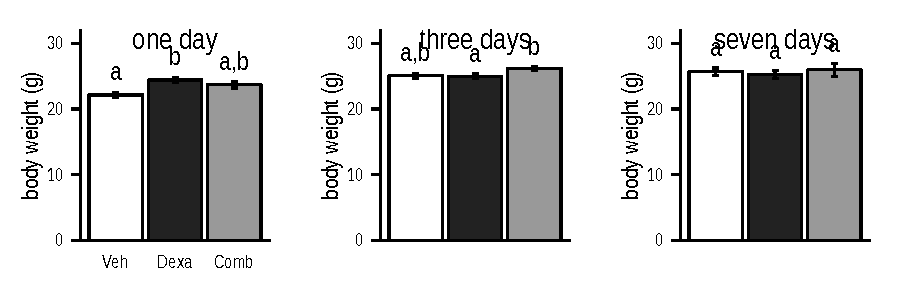
\includegraphics[width=6in,height=2.5in]{figure/unnamed-chunk-1-1} 

\end{knitrout}

\protect\caption[Body weight at sacrifice, following Dexa and / or Testo treatments.]{Body weight at sacrifice, following \SI{10}{\milli\gram\per\kilo\gram\per\day}
Dexa and / or \SI{28}{\milli\gram\per\kilo\gram\per\day} Testo treatments.
Treatments designated by the same letter do not differ significantly
from each other.\label{fig:Body-weight-at}}
\end{figure}


Upon finding the Dexa dose effective in inducing muscle atrophy, I
analyzed the body weight at sacrifice. There was no difference between
groups in terms of absolute weight, due to to the large variability
of the initial body weight (Fig. \ref{fig:Body-weight-at}, right).
The difference became apparent when percent change in body weight
was compared(Fig. \ref{fig:Time-course-of}, top, last time point).
In this case, the three treatments (vehicle, Dexa, or the combination
Dexa + Testo) were significantly different (Kruskal-Wallis p = 0.777).
Instead of the expected unchanged body weight over the seven days
of treatment with vehicle alone, there was a trend for growth, with
an apparent gain of 0.212
grams every day during the treatment. A similar trend has been seen
in the other repetitions of the experiment, as well as in other published
studies on young rodents. A sizable contribution to this growth was
brought by the 200 uL vehicle injected every day. Once this artifact
is taken into account, the gain of a negligible 0.0333
grams per day in the Dexa-treated group is in fact indicative of an
actual massive loss of body weight.

Seven-day weight gain in Dexa-treated group (1.05
± 1.14\%
of initial body weight) was significantly smaller than that of the
vehicle-treated group (6.12
± 0.879\%;
Dunn's test p = 0.0447).
Conversely, co-administration of Testo, hereafter termed \nomenclature{Comb}{combination of Dexa and Testo},
brought back the body weight gain over seven days to levels similar
to those in vehicle-treated animals (8.62
± 0.674\%;
Dunn's test vs. Dexa alone, p = 0.00167).

\begin{figure}
\begin{knitrout}
\definecolor{shadecolor}{rgb}{0.969, 0.969, 0.969}\color{fgcolor}
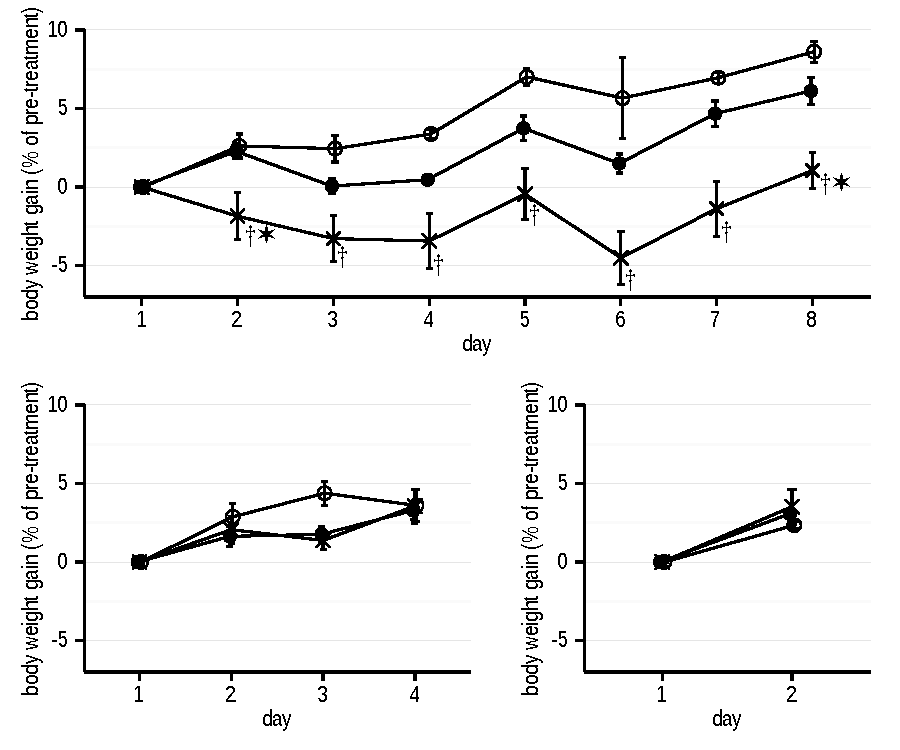
\includegraphics[width=6in,height=8in]{figure/unnamed-chunk-2-1} 

\end{knitrout}

\protect\caption[Time course of body weight Dexa and / or Testo treatments.]{Time course of body weight Dexa and / or Testo treatments. Stars
indicate statistically significant differences between Veh and Dexa
(p <0.05). Daggers indicate statistically significant differences
between Dexa and Comb (p <0.05).\label{fig:Time-course-of}}
\end{figure}


The time course of body weight changes revealed that both drugs' action
had a rapid onset (Fig. \ref{fig:Time-course-of}; Kruskal-Wallis
for first day percent change in body weight, p = 0.0239).
Specifically, mice receiving vehicle alone gained 2.28
± 0.485\%
body weight in the 24 hours, due to the significant mass of non-resorbable
corn oil. In contrast, mice receiving Dexa lost 1.86
± 1.5\%
body weight (Dunn's test p = 0.0387).
Mice receiving a combination of Dexa and Testo were essentially indistinguishable
from those receiving vehicle alone, having gained 2.61
± 0.767\%
body weight. This demonstrated an advantage of the combination treatment
over Dexa alone (Dunn's test p = 0.0213).

Based on the whole time course, I hypothesized that body weight changes
and muscle atrophy occur in a gradual manner, with significant metabolic
and molecular changes preceding the seven-day end of experiment. Accordingly,
I repeated the above experiment on different cohorts of mice, which
were sacrificed after only 1 or 3 days of treatment. Once more, absolute
changes in body weight could not be correlated with the muscle changes
(Fig. \ref{fig:Body-weight-at}, left and middle). When normalized,
relative changes in body weight for these groups of mice were less
ample than those seen with 7 days of treatment, to the point that
they were not statistically significant (Fig. \ref{fig:Time-course-of},
bottom). These shorter treatments provided insight into the molecular
development of atrophy, but, because they were run as independent
experiments, they will not be analyzed in conjunction.

Body composition analysis indicated that all animals included in these
experiments progressively lost total water. There was no difference
between water loss in the three experimental groups (Fig. \ref{fig:Changes-in-water,},
top; Kruskal-Wallis for seven day mass of water lost, p = 0.302).
This uniform loss of water negates a scenario in which the observations
could be ascribed to increased water retention due to non-specific
action of either steroid with MR. In all cases, the losses of total
water track the loss of lean body mass, indicating that muscle atrophy,
rather than renal dysfunction, underlies the loss of water. Fat mass
analysis indicated that in the vehicle-alone treated group, the rate
of apparent fat gain was essentially equal with the mass of injected
vehicle accrued over the seven days. This demonstrates that experiments
manipulations, in the absence of pharmacological treatments, have
no effect on lipid metabolism. Dexa-treated groups accrued more fat
(Dunn's test, vehicle vs. Dexa, p = 0.0681;
Dunn's test, vehicle vs. combination, p = 0.0172).
Testo co-administration had little effect on lipid metabolism(Dunn's
test, Dexa vs. combination, p = 0.802).

Even ampler changes were induced by the two drugs on lean body mass
(Fig. \ref{fig:Changes-in-water,}, bottom; Kruskal-Wallis for seven
day lost lean mass , p = 0.000811).
Vehicle alone has no effect on lean body mass (0.0467
± 0.029
grams per day loss over seven days). The massive loss of lean body
mass (0.459
± 0.0237
grams per day) becomes significantly different from control by the
third day (Dunn's test, p = 0.000242).
When Testo was co-administered, the loss of lean body mass persisted,
but there was a trend towards a lower loss rate{ (}0.224
± 0.029
grams per day; Dunn's test, Dexa vs. combination, p = 0.108).

\begin{figure}
\begin{knitrout}
\definecolor{shadecolor}{rgb}{0.969, 0.969, 0.969}\color{fgcolor}
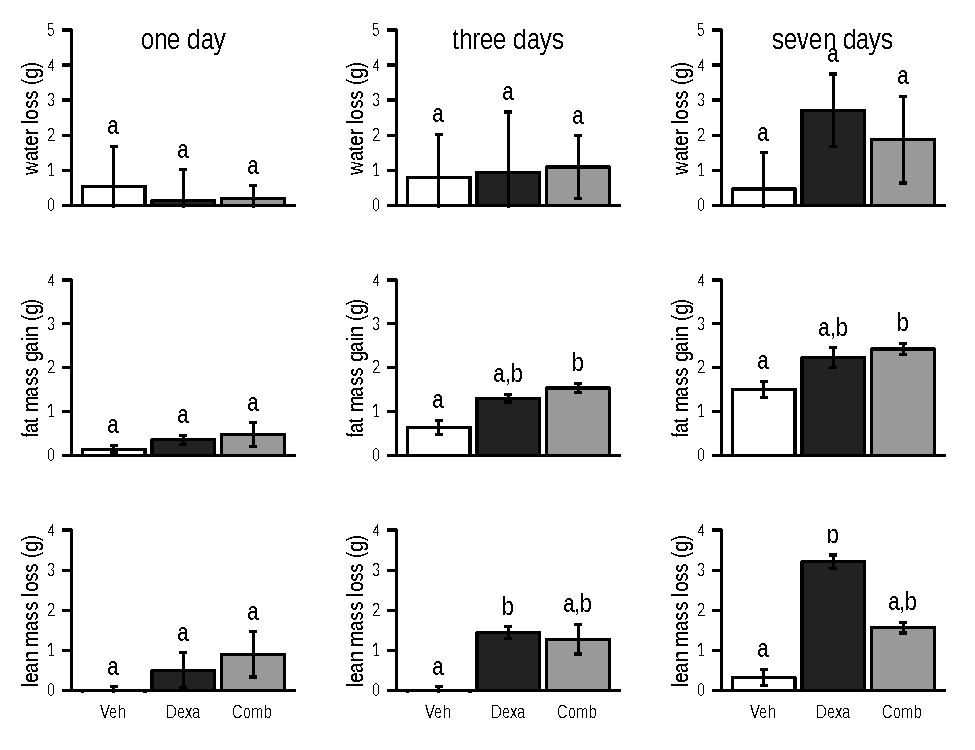
\includegraphics[width=6in,height=8in]{figure/unnamed-chunk-3-1} 

\end{knitrout}

\protect\caption{Changes in water, lean, and fat body mass, after Dexa and / or Testo
treatments.\label{fig:Changes-in-water,}}
\end{figure}
Dissection of individual muscles confirmed that Dexa achieved widespread
muscle atrophy.\pagebreak{}


\chapter{In vitro findings}

todo

\begin{singlespace}
\pagebreak{}
\end{singlespace}


\chapter{Discussion}

todo


\section{Conclusions}


\section{Future directions}

todo

\begin{singlespace}
\pagebreak{}
\end{singlespace}

\bibliographystyle{3_dump_writingswork_draftthesis_nihunsrt}
\phantomsection\addcontentsline{toc}{chapter}{\bibname}\bibliography{2_dump_writingswork_draftthesis_thesis}


\begin{singlespace}
\pagebreak{}
\end{singlespace}


\chapter{Curriculum vitae}


\section*{Nicolae Lucian Sandor}


\subparagraph*{Education}
\begin{itemize}
\item PhD candidate, Boston University School of Medicine, expected graduation
2015
\item BS (Licentiat in Biofizica), Universitatea Bucuresti, 2005
\item BM\textbackslash{}DM (Doctor in Medicina), Universitatea de Medicina
si Farmacie Carol Davila Bucuresti, 2002
\end{itemize}

\subparagraph*{Research experience}
\begin{itemize}
\item 2012-2015: Department of Medicine, Boston University School of Medicine,
P.I. Dr. Shalender Bhasin, under the supervision of Dr. Carlo Serra

\begin{itemize}
\item Subject: Testosterone alleviating glucocorticoid-induced muscle loss.
\end{itemize}
\item 2009-2012: Department of Biophysics, Boston University School of Medicine,
P.I. Dr. Assen Marintchev

\begin{itemize}
\item Subject: Interactions between translation initiation factors eIF1A
and eIF5B
\end{itemize}
\item 2005-2008: Center for the Study of Brain, Mind and Behavior, Princeton
University, P.I. Dr. Anne Treisman, FRS

\begin{itemize}
\item Subject: Brain mechanisms for statistical processing of visual scenes
\end{itemize}
\item Summer 2004: Biology Department, Universitatea Bucuresti, P.I. Dr.
Gordon Reid, under the supervision of Dr. Iurie Barbu

\begin{itemize}
\item Subject: The mediation of thermoception by ionic membrane channels
\end{itemize}
\item 2001-2002: Biophysics Department, Universitatea de Medicina si Farmacie
Carol Davila Bucuresti, P.I. Dr. Dan Eremia, under the supervision
of Dr. Eva Katona, 

\begin{itemize}
\item Subject: The effect of non-ionizing radiation of the mobility of the
cell membrane lipids
\end{itemize}
\end{itemize}

\subparagraph*{Peer-reviewed publications}
\begin{enumerate}
\item Serra C, Tangherlini F, Rudy S, Lee D, Toraldo G, Sandor NL, Zhang
A, Jasuja R, Bhasin S. \emph{Testosterone improves the regeneration
of old and young mouse skeletal muscle}. J Gerontol A Biol Sci Med
Sci. 2013 Jan;68(1).
\item Serra C, Sandor NL, Jang H, Lee D, Toraldo G, Guarneri T, Wong S,
Zhang A, Guo W, Jasuja R, Bhasin S. \emph{The effects of testosterone
deprivation and supplementation on proteasomal and autophagy activity
in the skeletal muscle of the male mouse: differential effects on
high-androgen responder and low-androgen responder muscle groups}.
Endocrinology. 2013 Dec;154(12).
\item Guo W, Bachman E, Vogel J, Li M, Peng L, Pencina K, Serra C, Sandor
NL, Jasuja R, Montano M, Basaria S, Gassmann M, Bhasin S. \emph{The
effects of short-term and long-term testosterone supplementation on
blood viscosity and erythrocyte deformability in healthy adult mice}.
Endocrinology. 2015 Mar 16;en20141784. PMID: 25774550.
\end{enumerate}

\subparagraph*{Other scientific communications}
\begin{enumerate}
\item Sandor NL, Hendrickson E, Sandor D, Wagner G, Pestova TV, Marintchev
A. \emph{Interplay between intra- and intermolecular interactions
involving human eIF1A and eIF5B}. Abstract presented at the 2010 Meeting
of Translational Control, Sept. 2010, Cold Spring Harbor, NY.
\item Sandor NL, Lee D, Toraldo G, Zhang A, Jasuja R, Bhasin S, Serra C.
\emph{The role of testosterone on the control of muscle protein synthesis
and degradation}. Abstract presented at the 2011 Evans Center Days,
Nov. 2011, Boston, MA.
\item Serra C, Lee D, Sandor NL, Toraldo G, Jang H, Jasuja R, Bhasin S.
\emph{Characterization of the neuromuscular junction in castrated
male mice}. Poster presented at ENDO2013, The Endocrine Society's
95th Annual Meeting \& Expo, 2013, San Francisco, CA.
\item Sandor NL, Jasuja R, Serra C, Bhasin S. \emph{Testosterone alleviates
glucocorticoid myopathy by inhibiting the proteolytic machinery}.
Poster presented at the 2013 Evans Center Days, Nov. 2013, Boston,
MA.
\end{enumerate}



\end{document}
